\documentclass [a4paper,11pt]{book}
\usepackage[a4paper,plainpages=false,pdfpagelabels]{hyperref}

\usepackage[T1]{fontenc}
\usepackage[utf8]{inputenc}
\usepackage{lmodern}

\usepackage[font=small,labelfont=bf]{caption}
\usepackage{subfiles}

%%%%%%%%%
\usepackage{cite}
\usepackage{color}
\usepackage{units}
\usepackage{bold-extra}
\usepackage{array}
\usepackage{calc}
\newcolumntype{N}{@{}m{0pt}@{}}

\setcounter{secnumdepth}{4}
\setcounter{tocdepth}{4}
\setcounter{secnumdepth}{4}

\usepackage{float}

\usepackage{pbox}

\usepackage[titletoc]{appendix}

\usepackage[framemethod=tikz]{mdframed}
\global\mdfdefinestyle{defStyle}{%
leftmargin=1cm,%
rightmargin=1cm,%
roundcorner=1,%
frametitlealignment=\center
}

\usepackage{amsmath}
\usepackage{listings}
\usepackage{cite}
\usepackage{url} 
\usepackage{graphicx}
\usepackage{fancyhdr}
\usepackage[italian]{babel}
\usepackage{fixltx2e}
\usepackage[labelfont=bf]{caption}
\usepackage{float}
\usepackage[utf8]{inputenc}
\usepackage{geometry}
\graphicspath{{images/}}
\captionsetup{labelfont=bf}
\pagestyle{fancy}
\fancyhf{} %
\fancyhead[LE]{\bfseries\leftmark}
\fancyhead[RO]{\bfseries\rightmark}
\fancyfoot[C]{\thepage}

\def\signed #1{{\leavevmode\unskip\nobreak\hfil\penalty50\hskip2em
  \hbox{}\nobreak\hfil(#1)%
  \parfillskip=0pt \finalhyphendemerits=0 \endgraf}}

\newsavebox\mybox
\newenvironment{aquote}[1]
  {\savebox\mybox{#1}\begin{quote}}
  {\signed{\usebox\mybox}\end{quote}}
%%%%%%%%
\usepackage{setspace}
\linespread{1.2}


\begin{document}

%%%%%%%%
\frontmatter

% Create a new page
\newpage
% Set borders
\newgeometry{top=3cm,bottom=3cm,inner=2.7cm,outer=2.7cm}
% Remove page number
\thispagestyle{empty}
% Remove default indentation of paragraph
\noindent
% Move the content a bit on the left
\hspace*{-1mm}
% Include the logo

\includegraphics[width=0.2\columnwidth]{source/immagini/logo-bicocca-gray.jpg}
% Place some space between text and image
\hspace*{2mm}
% Open a box in which place the header
% use \par to space the lines
\begin{minipage}[b][][c]{0.8\columnwidth}
\begin{spacing}{1.4}
{\large\textsc{Universit\'a degli Studi di Milano Bicocca}\par}
{\large\textbf{Scuola di Scienze}\par}
{\large\textbf{Dipartimento di Scienze dei Materiali}\par}
{\large\textbf{Corso di Laurea in Ottica e Optometria}\par}
\end{spacing}
\end{minipage}
% Vertical fill space
\vfill


\begin{center}
{\Huge\textsc{\textbf{Correlazione tra sistema visivo e apparato stomatognatico }}\par}
\end{center}
% Fill the remaining space
\vfill
\large
% Place the advisor under title, on the left
\begin{flushleft}
\textbf{Relatore:}\\
\hspace*{2em}\textit{Prof.} Maurizio \textsc{Acciarri}
\end{flushleft}
% Place co-advisors under advisor
\begin{flushleft}
\textbf{Co-relatore:}\\
\hspace*{2em}\textit{Prof.ssa} Nadia \textsc{Mattioli}\\
\end{flushleft}
% Leave some space
\vskip 1cm
% Write candidate on the right
\begin{flushright}
\textbf{Relazione della prova finale di:}\\
\hspace*{2em}Serena \textsc{Delbono}\\
\hspace*{2em}Matricola 782525

\textbf{ \\ Appello di laurea:}\\
\hspace*{2em}16 Marzo 2017
\end{flushright}
\vfill
% Place year at bottom
\begin{center}
\textsc{\textbf{Anno Accademico 2015-2016}}
\end{center}
\restoregeometry

\thispagestyle{empty}
\cleardoublepage
\newpage
\tableofcontents

\newpage
\listoffigures
\listoftables

%%%%%%%%%%%%%%%%%%%


\mainmatter
\chapter*{Introduzione}
\addcontentsline{toc}{chapter}{Introduzione}





Gli studi condotti negli ultimi anni hanno posto l'attenzione su come il nostro corpo sia funzionalmente collegato e le sue parti si influenzino reciprocamente. Questa relazione funzionale non si attua tra singoli elementi, come occhio e lingua, ma tra sistemi, come visivo e stomatognatico. Poichè sono inclusi in un sistema più complesso, quale è il nostro corpo, esso si adatta ai cambiamenti in modo diverso per ognuno di noi\footnote{\emph{Occlusione vs oculomotricità: stato dell'arte} di Giorgetti, Deodato, Malpassi}.
\\\
Il corpo recepisce le informazioni su come organizzarsi nello spazio da stimoli provenienti dal mondo esterno. Attraverso questo meccanismo stimolo-risposta si sviluppa la postura corporea. Dal punto di vista motorio il corpo si adatta agli stimoli esterni per sopravvivere e svolgere le sue attività, questo porta ad assumere quindi la postura più consona alla situazione e alle proprie esigenze. 
\\\
La funzione di informare i sistemi è affidata al Sistema-Tonico-Posturale \emph{S.T.P.} costituito da un insieme di strutture comunicanti. L'S.T.P. necessita di un input che proviene dagli estrocettori e propriocettori (esempio: occhio,bocca, piede, pelle, muscoli), il quale viene rielaborato e trasformato in output che traduce in gesto motorio il segnale\footnote{\url{http://www.associazioneitalianastudioericercaposturologia.it/allegati/Articolo\%20AIP\%20Salvatore\%20Mautone.pdf}}.
\\\
L'occhio fornisce al cervello la maggior parte delle informazioni che servono per interpretare lo spazio che ci circonda, quindi una disfunzione del sistema visivo può provocare degli squilibri nei vari sistemi e viceversa. In particolare in vari studi è stato evidenziato come ci sia un collegamento tra le malocclusioni e i difetti di convergenza. Sembra infatti che disfunzioni dell'apparato stomatognatico influenzino le funzionalità del sistema visivo, portando ad adattamenti della postura del capo\footnote{Armando Silvestrini-Biavati, Marco Migliorati, Eleonora Demarziani, Simona Tecco, Piero Silvestrini-Biavati, Antonella Polimeni and Matteo Saccucci \emph{Clinical association between teeth malocclusions, wrong posture and ocular convergence disorders: an epidemiological investigation on primary school children}}\footnote{Antonino Marco Cuccia e Carola Caradonna \emph{Binocular motility system and temporomandibular joint internal derangement: A study in adults}}. 


È in questo contesto che si colloca questo studio, basato sull'assunzione che dalla disfunzione dell'apparato stomatognatico si ottiene l'adattamento da parte degli altri sistemi, in particolare del sistema visivo. Per ottenere i risultati si vuole osservare se e come cambia il sistema visivo in soggetti con disfunzioni generali primarie dell'apparato stomatognatico (masticazione, deglutizione, respirazione) dopo aver seguito un trattamento logopedico e osteopatico. Il trattamento prevede l'utilizzo della Terapia Miofunzionale, cioè un percorso terapeutico volto ad insegnare la corretta posizione della lingua sia durante il riposo, che durante la deglutizione per portare al riequilibrio della funzione della muscolatura oro-facciale. La terapia viene svolta con l'insegnamento di esercizi volti al rilassamento, allungamento e rinforzo dei muscoli coinvolti nelle funzioni orali.  Viene poi integrata con delicate manipolazioni eseguite prevalentemente nei distretti di cranio, collo e torace con l'obiettivo di rilasciare le tensioni muscolari presenti.
\\\
Lo svolgimento della ricerca è avvenuto effettuando una valutazione optometrica pre e post trattamento, osservando diverse componenti del sistema visivo, tra cui il difetto refrattivo, la stabilità, l'oculomotricità, la convergenza e l'accomodazione.
L'obiettivo è verificare che l'occhio sia correlato al resto del corpo e in particolare all'apparato stomatognatico, attraverso strutture che sono in continuo adattamento per ricercare sempre l'equilibrio complessivo e comprendere quali sono le caratteristiche visive maggiormente collegate. 
\\\
In questa ricerca si è rivelato fondamentale il confronto con vari professionisti, inquadrando il lavoro in un approccio multidisciplinare.


I contenuti della ricerca saranno divisi in 3 capitoli. Nel primo capitolo verranno esposte le caratteristiche del sistema visivo dal punto di vista anatomico e fisiologico, con annessa la descrizione delle funzionalità analizzate durante la ricerca. Nel secondo si porrà l'attenzione sulla postura e sull'apparato stomatognatico, descrivendo i collegamenti anatomici e fisiologici che lo legano al sistema visivo. Nel terzo capitolo verranno descritti lo svolgimento e i risultati ottenuti dallo studio effettuato, concludendo con le considerazioni e proponendo eventuali sviluppi futuri.


\chapter{Sistema visivo}

L’apparato visivo, tra tutti quelli presenti nel corpo umano, è il più complesso ed ha la massima importanza perché è quello che più di altri ci permette di conoscere il mondo esterno. Questo avviene perché esso non provvede solo alla percezione qualitativa e quantitativa della luce, ma trasmette anche le informazioni al cervello in segnali topograficamente organizzati in modo tale che la recezione si traduce in immagini sufficientemente fedeli di ciò che stiamo osservando. Esso permette quindi lo sviluppo della visione, in quanto capacità di interpretare e capire ciò che vediamo.

Gli elementi anatomici che compongono l’apparato visivo sono: bulbo oculare ed organi accessori (cristallino, apparato oculomotore, palpebre, ghiandole lacrimali, congiuntiva).

Di seguito verranno analizzate le componenti coinvolte nel movimento dell’occhio, nella formazione dell’immagine e verrà descritto come sono innervate. Seguirà  poi un approfondimento sulle caratteristiche funzionali del sistema visivo.
\\\ \\\
\section{Anatomia e fisiologia}

\subsection{Bulbo oculare}

Il bulbo oculare (Figura 1.1) si trova nella parte anteriore della cavità orbitaria decentrato in alto e verso l’esterno rispetto alle pareti e mantenuto in sito da connessioni muscolari, vascolari e dal nervo ottico. È inoltre appoggiato ad una formazione membranosa connettivale detta fascia del bulbo. 

Il bulbo oculare è una formazione sferoidale che contiene materiali liquidi, semi-liquidi e solidi fasciati da diverse membrane di copertura dette tonache. All’esterno si trova la tonaca fibrosa, formata dalla sclera e dalla cornea, poi la tonaca vascolare, ricchissima di vasi per irrorare e pigmentazione per permettere la creazione di una camera oscura nell’occhio, infine, all’interno, la tonaca nervosa (retina) che contiene i fotorecettori responsabili della trasformazione del segnale luminoso in segnale elettrico.

Il bulbo è diviso in due camere: la camera anteriore che contiene umor acqueo e la camera posteriore che contiene umor vitreo. Le camere sono separate dall’iride: un disco portante al centro il forame pupillare, il quale gestisce la quantità di luce da far entrare nell’occhio. Dietro l’iride si trova il cristallino, supportato dai processi ciliari, il quale è in grado di cambiare la sua forma perché avvenga il processo di accomodazione, cioè la messa a fuoco a diverse distanze.

\\\


\begin{figure}[h!]
\centering
\begin{minipage}{.5\textwidth}
  \centering
  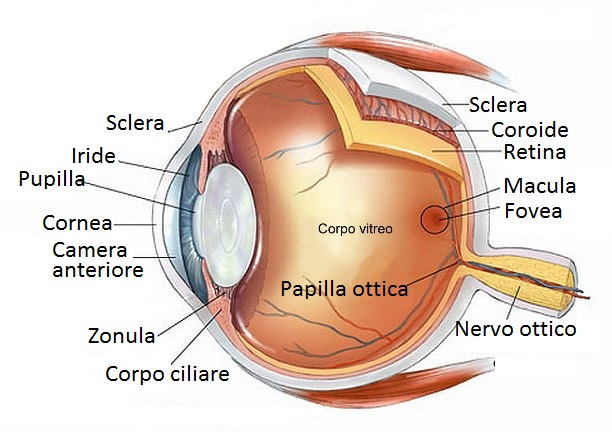
\includegraphics[scale=1.0]{source/immagini/anatomia_occhio.jpg}
  \captionof{figure}{Sezione del bulbo oculare.}
  \label{fig:test1}
\end{minipage}%
\begin{minipage}{.5\textwidth}
  \centering
  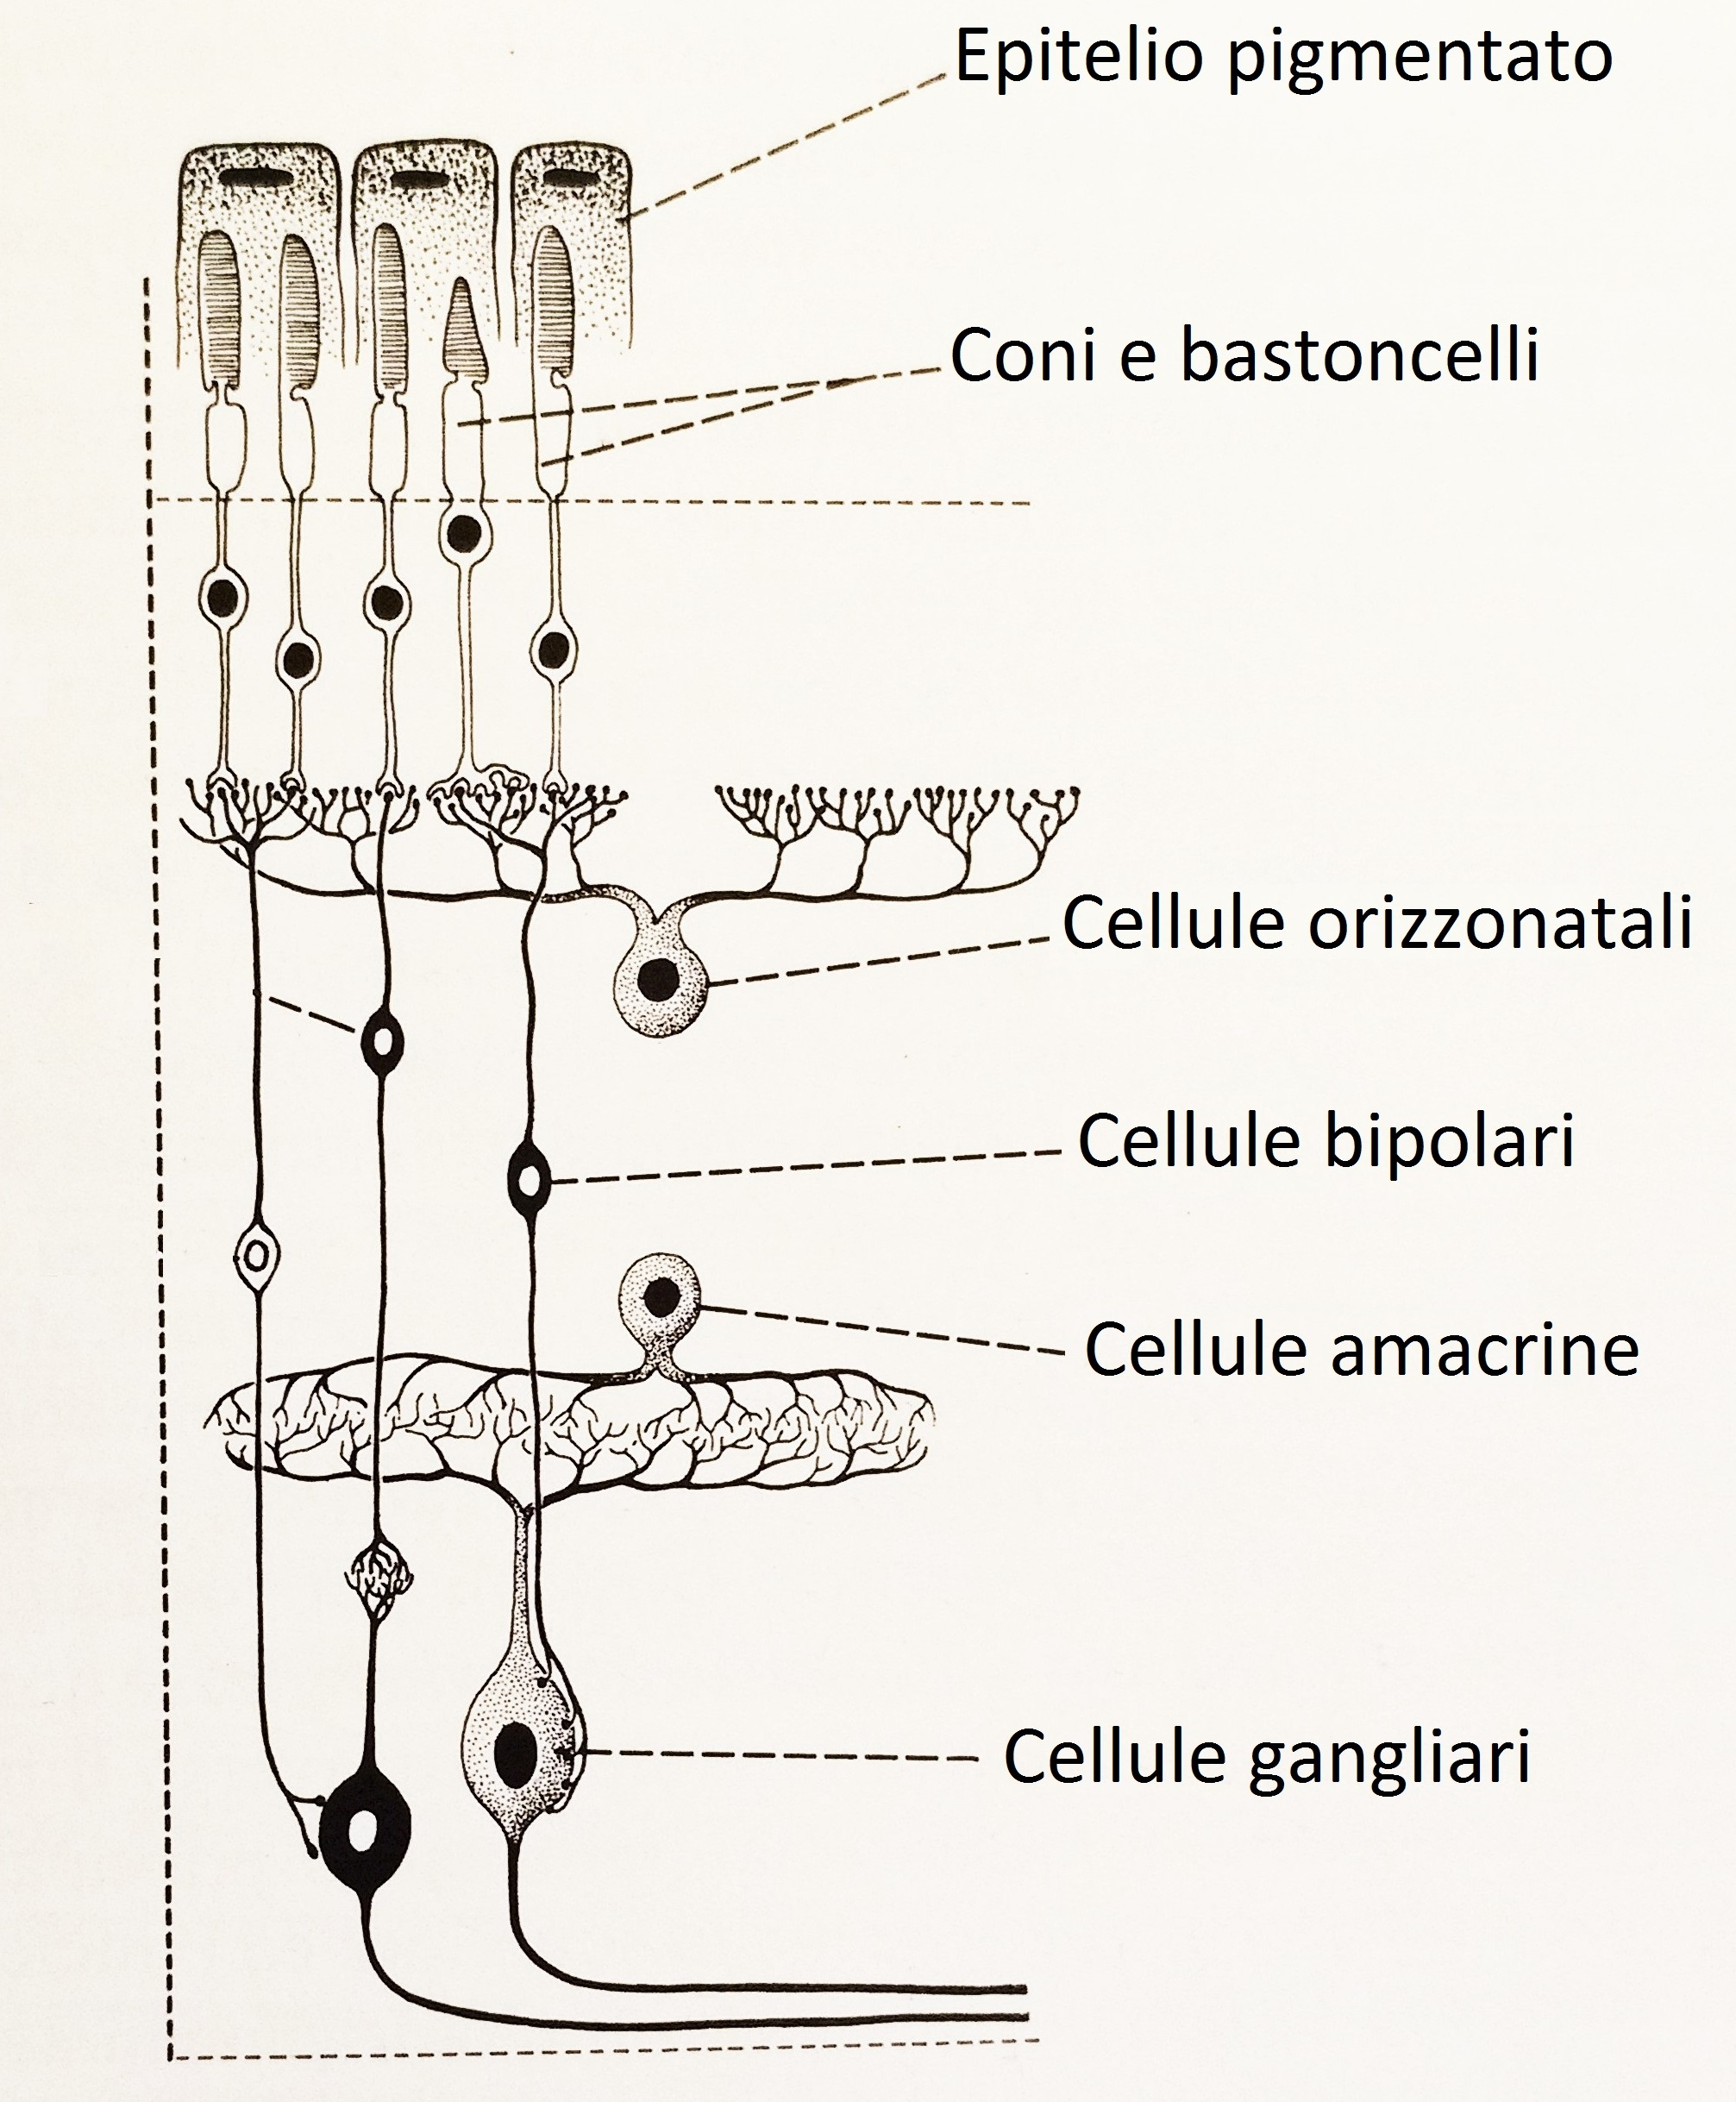
\includegraphics[scale=0.08]{source/immagini/retina.jpg}
  \captionof{figure}{Stratificazione della retina.}
  \label{fig:test2}
\end{minipage}
\end{figure}


\subsection{Generazione dell'immagine retinica}

Quando la luce colpisce l’occhio deve attraversare la cornea, la pupilla e il cristallino, che permettono di focalizzarla su diverse parti della retina. La zona della retina in cui vengono codificati i dettagli e i colori è la fovea, dove si concentrano i fotorecettori coni. Perifericamente invece, sono presenti maggiormente i fotorecettori bastoncelli, i quali sono adibiti alla percezione della luminosità e del movimento. I coni e i bastoncelli hanno il compito di trasformare il segnale luminoso in segnale elettrico attraverso una serie di eventi biochimici a cascata. Il segnale viene poi trasmesso alle cellule bipolari e ganglionari, come si vede in Figura 1.2. Di quest'ultime ne esistono diversi tipi che raccolgono le diverse caratteristiche dell’immagine visiva, come luminosità, colore o movimento. Gli assoni delle cellule ganglionari si uniscono per formare il nervo ottico, il quale giunge al chiasma ottico dove avviene una parziale decussazione delle fibre ottiche: quelle provenienti dalla metà nasale della retina passano nel tratto ottico del lato opposto, che contiene quindi fibre omolaterali della metà temporale e fibre controlaterali della metà nasale. Le fibre si dirigono poi al Nucleo Genicolato Laterale, al collicolo superiore e al pretetto. 
\\\
Vi sono diverse vie visive in base all’informazione da codificare: la via dalla retina al corpo genicolato laterale, la via retino-pretettale e la via retino-collicolare.
\\\ \\\ \\\ 
\textbf{Via retina-corpo genicolato laterale}: 
\\\
Al corpo genicolato laterale, nel talamo situato nel tronco encefalico (Figura 1.3), arrivano le sole fibre adibite alla percezione visiva. Da qui si dipartono neuroni secondari che arrivano alla corteccia visiva primaria (V1), dalla quale si dipartono la via ventrale e la via dorsale che portano alle aree visive superiori, che sono specializzate funzionalmente. La via ventrale termina nel lobo temporale inferiore ed è adibita alla percezione dell’oggetto: colore, forma, trama, riconoscimento, visi. La via dorsale termina nel lobo parietale ed è adibita alla percezione spaziale, quindi la percezione delle differenze di luminosità, ma non di colore.
Le fibre che entrano a far parte delle vie riflesse, non si arrestano al corpo genicolato laterale, ma si portano al mesencefalo, terminando in due territori: pretetto (Figura 1.4) e collicolo superiore.
\\\ \\\ \\\
\textbf{Via retino-pretettale}: 
\\\
Per il controllo dei riflessi pupillari le fibre delle cellule ganglionari adibite alla luminosità giungono al pretetto, zona formata da un gruppo di nuclei posti anteriormente e superiormente al collicolo superiore, nel punto in cui il mesencefalo si continua con il talamo. Le cellule di quest’area proiettano l’informazione ai nuclei di Edinger-Westphal, dal quale i neuroni raggiungono il muscolo sfintere dell’iride, unendo i loro assoni con il nervo oculomotore (Figura 1.4).

\begin{figure}[h!]
	\centering
	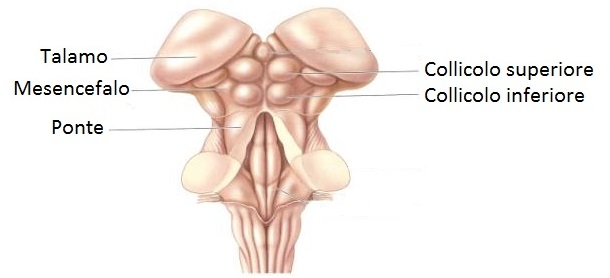
\includegraphics[scale=0.52]{source/immagini/tronco_encefalico.jpg}
	\caption[Tronco encefalico]{Tronco encefalico.}
	\label{fig:test3}
\end{figure}
\\\ \\\ 
\textbf{Via retino-collicolare}: 
\\\
Per il controllo dei movimenti rapidi degli occhi le vie passano dal collicolo superiore, nel mesencefalo (Figura 1.3), diviso in sette strati in cui sono rappresentate le mappe sensoriali. Al collicolo giungono informazioni provenienti anche da altri sensi permettendogli di dirigere i movimenti oculari in direzione dello stimolo, indipendentemente dalla sua natura.
\end{itemize}


\begin{figure}[h!]
	\centering
	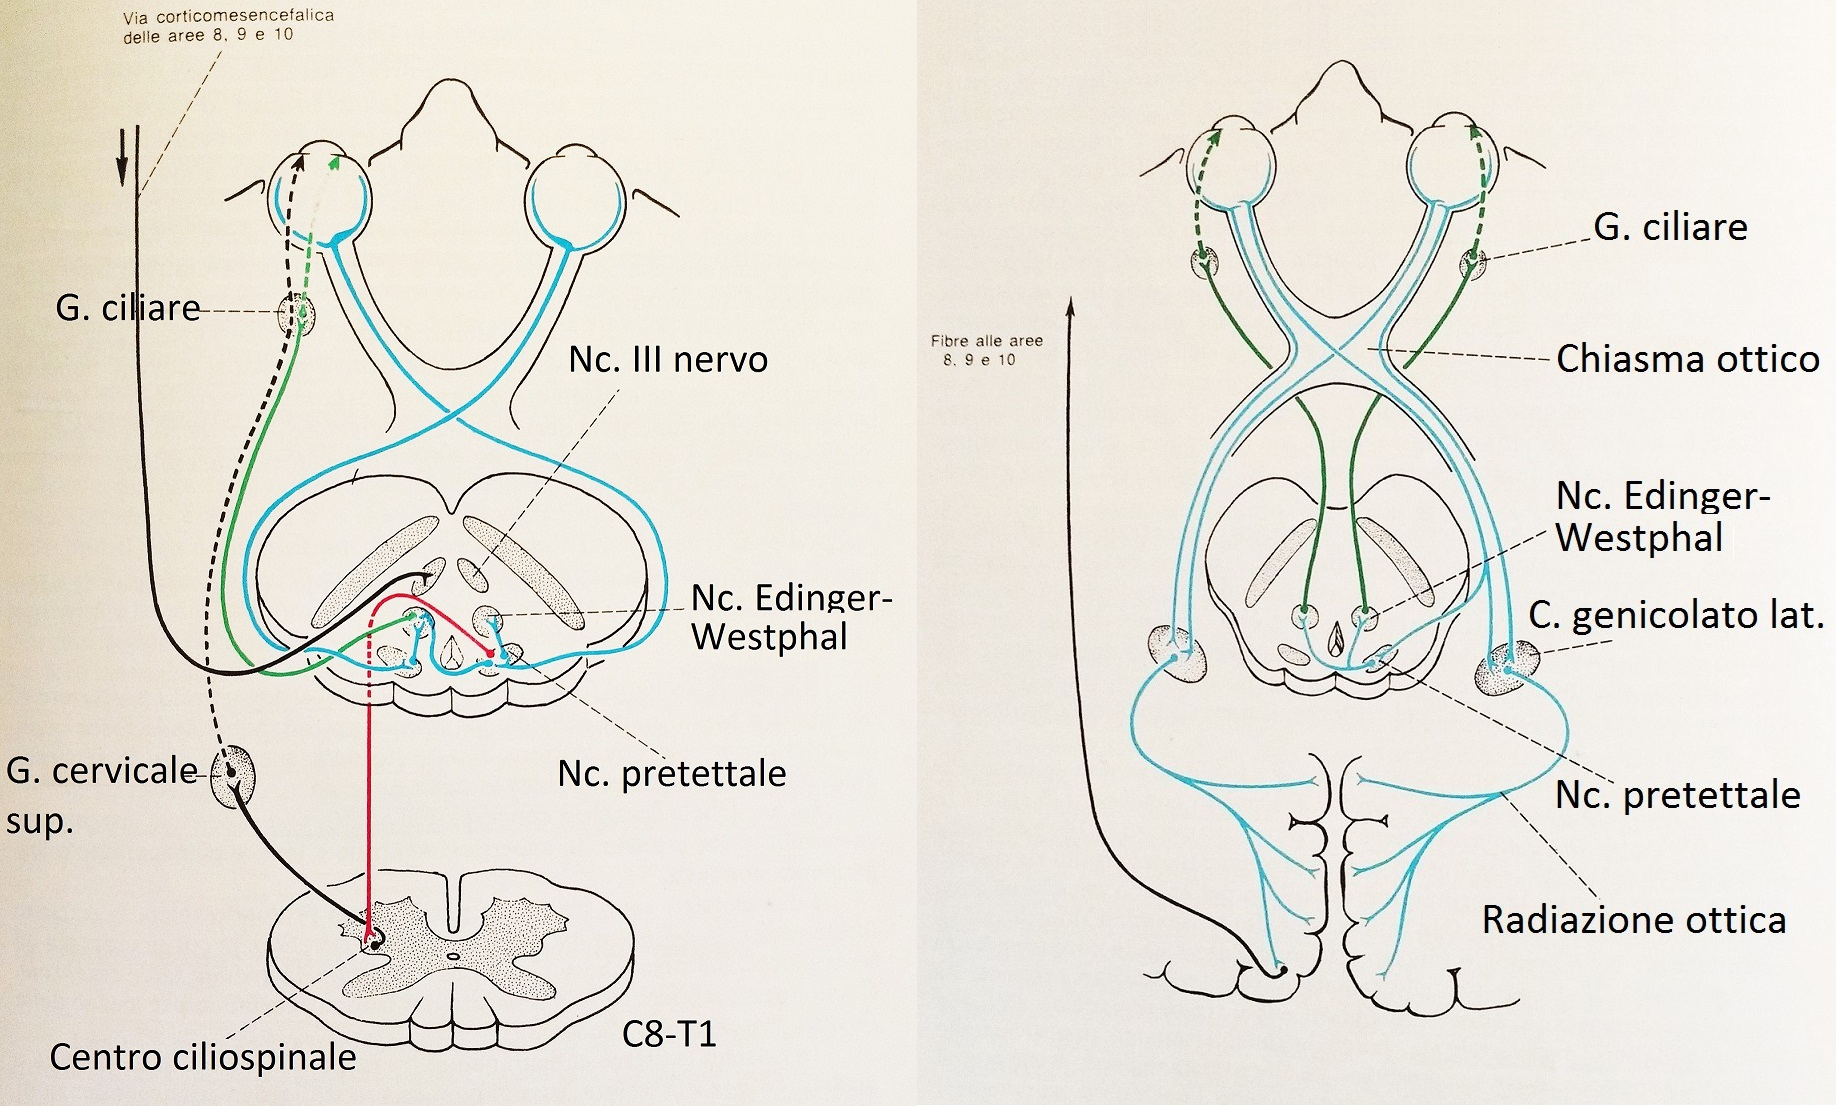
\includegraphics[scale=0.40]{source/immagini/vie_visive.png}
	\caption[Rappresentazione delle vie visive]{Rappresentazione vie visive: a sinistra la via pretettale e collicolare, a destra la via del nucleo genicolato laterale e pretettale.}
	\label{fig:test3}
\end{figure}

\subsection{Apparato muscolare dell'occhio}

L’apparato muscolare dell'occhio è costituito da una muscolatura estrinseca ed una intrinseca e svolge diverse funzioni: amplia il campo visivo, consente la fissazione foveale e la visione binoculare singola, fornisce la consapevolezza spaziale e stabilisce l'immagine retinica.
\\\
 
Il movimento oculare è permesso dai muscoli estrinseci (Figura 1.5) i quali partono dalla profondità dell’orbita dove si trova un anello fibroso detto anello tendineo di Zinn. Da esso partono sei muscoli: quattro retti (inferiore, mediale, laterale e superiore), il muscolo obliquo superiore ed il muscolo elevatore della palpebra. C’è un ulteriore muscolo, l’obliquo inferiore, che però parte più avanti dell’anello tendineo. Il compito di questi muscoli è quello di permettere il movimento del globo e di mantenerlo sospeso all’interno di un sistema di tessuti connettivi estesi tra l’apice dell’orbita e le rime palpebrali. I muscoli retti, con i loro annessi, costituiscono un cono muscolare attraversato dal nervo ottico, vasi sanguigni e nervi. Lo spazio rimanente è riempito dai grassi retro bulbari. 
\\\
\begin{figure}[h!]
	\centering
	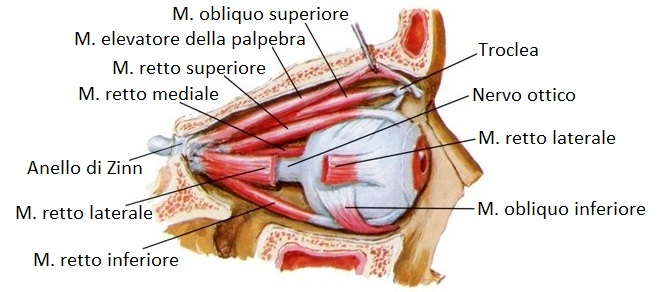
\includegraphics[scale=2.7]{source/immagini/muscoli_estrinseci_occhio.jpg}
	\caption[Muscoli estrinseci dell'occhio]{Muscoli estrinseci dell'occhio.}
	\label{fig:test6}
\end{figure}

Il bulbo oculare è in grado di svolgere rotazioni attorno a tre assi: orizzontale $Z$, verticale $X$ e antero-posteriore $Y$ detti \emph{Assi di Fick} (Figura 1.6). Gli assi $Y$ e $Z$ giacciono sul piano equatoriale detto \emph{Piano di Listing}. Se l’occhio non compie alcuna rotazione si dice che si trova in posizione primaria, se ruota intorno ad un asse del piano di Listing  è in posizione secondaria, se invece ruota contemporaneamente intorno ad $X$ e $Z$ è in posizione terziaria.

\begin{figure}[h!]
	\centering
	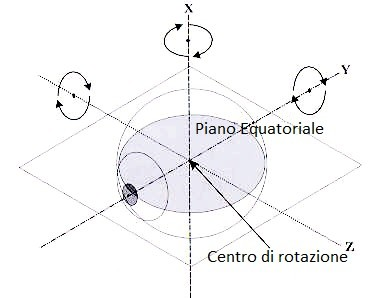
\includegraphics[scale=0.49]{source/immagini/Assi.jpg}
	\caption[Assi di Fick]{Assi di Fick.}
	\label{fig:test7}
\end{figure}
\\\  \\\
L’occhio può compiere rotazioni intorno agli assi verticale e orizzontale dette duzioni:
 \begin{itemize}
 \itemsep-0.7em 
 \item[--]asse orizzontale $Z$: elevazione e abbassamento
 \item[--]asse verticale $X$: adduzione e abduzione.
 \item[--]asse antero-posteriore $Y$: extorsione (movimento che porta il polo superiore della cornea verso il lato temporale) e intorsione (movimento che porta il polo superiore della cornea verso il lato nasale)
 \end{itemize}
\\\ \\\
\textbf{Muscoli Retti orizzontali}
\\\
I muscoli retti laterale e mediale in contrazione determinano la rotazione dell’occhio attorno all’asse X, producendo Adduzione (retto mediale) e Abduzione (retto laterale).
\\\ \\\	
\textbf{Muscoli Retti verticali}
\\\
Con l’occhio in posizione primaria di sguardo i muscoli retti verticali hanno gli assi che formano 23$^{\circ}$ con l’asse visivo (Figura 1.7), quindi non ci sarà un movimento di pura elevazione o puro abbassamento, ma mista. Quando l’occhio è abdotto di 23$^{\circ}$ allora ci sarà movimento di pura elevazione quando si contrae il muscolo retto superiore e puro abbassamento quando si contrae il retto inferiore.
\\\ \\\
\textbf{Muscoli Obliqui}
\\\ 
In posizione primaria di sguardo l’asse muscolare forma un angolo di 53$^{\circ}$ con l’asse visivo, come mostrato in Figura 1.8, quindi in questa posizione la loro azione sarà molteplice. Obliquo superiore avrà come azione primaria l’incicloduzione, secondaria la depressione e terziaria l’abduzione. L’obliquo inferiore avrà azione primaria l’excicloduzione, secondaria l’elevazione e terziaria l’abduzione. 

\begin{figure}[h!]
\centering
\begin{minipage}{.5\textwidth}
  \centering
  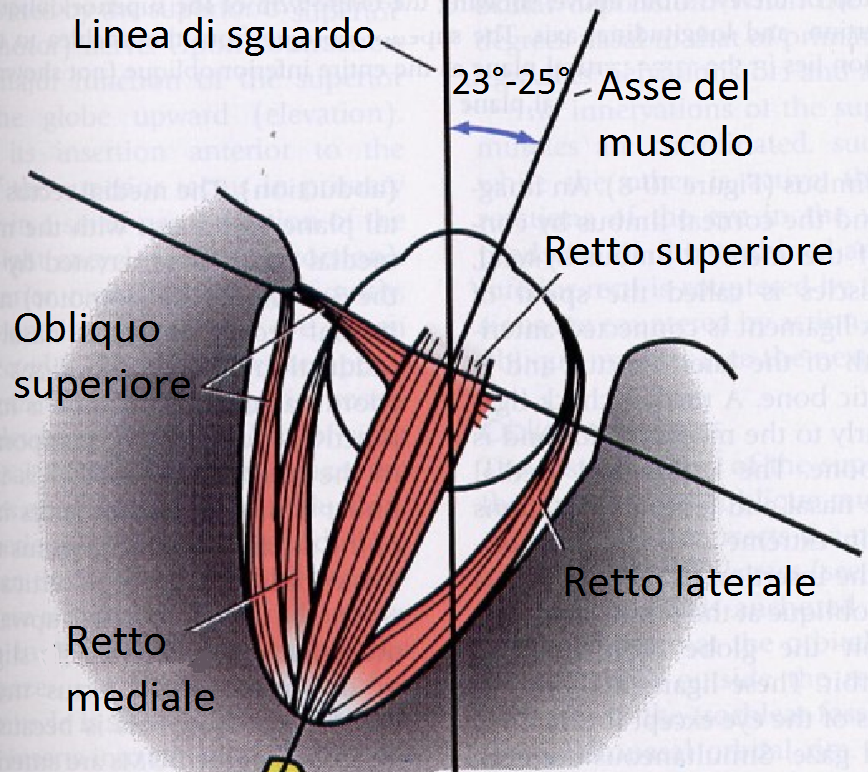
\includegraphics[scale=0.34]{source/immagini/Assi_retti.png}
  \captionof{figure}{Asse del muscolo retto.}
  \label{fig:test8}
\end{minipage}%
\begin{minipage}{.5\textwidth}
  \centering
  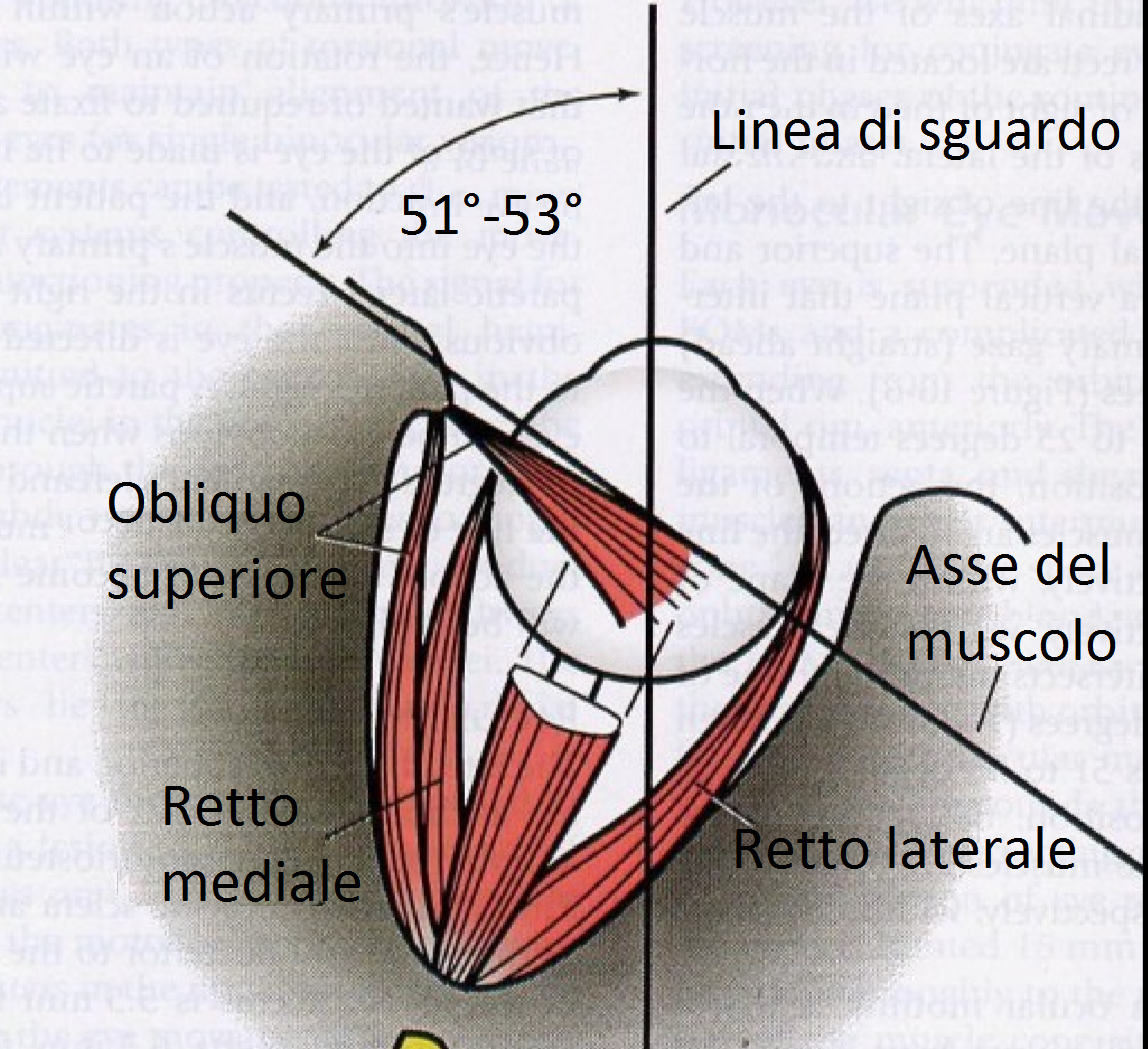
\includegraphics[scale=0.25]{source/immagini/Assi_obliqui.png}
  \captionof{figure}{Asse del muscolo obliquo.}
  \label{fig:test9}
\end{minipage}
\end{figure} 


  
\subsection{Innervazione del sistema visivo}

L’innervazione del sistema visivo è costituita dai nervi encefalici. In generale ci sono 12 nervi encefalici, ma quelli adibiti al sistema visivo sono cinque: II paio o nervo ottico, III paio o nervo oculomotore comune, IV paio o nervo trocleare, V paio o nervo trigemino, VI paio o nervo abducente.
\\\ \\\
\textbf{Nervo ottico (II paio)}
\\\ 
Esso prende origine dalla papilla del nervo ottico, costituito dall’unione degli assoni delle cellule gangliari della retina, abbandona il bulbo oculare e si incontra nel chiasma ottico con il nervo ottico dell'altro occhio per scambiarsi le fibre. Proseguono poi nei tratti ottici che giungono nei corpi genicolati laterali del diencefalo.
\\\ \\\
\textbf{Nervo oculomotore comune (III paio)}: 
\\\ 
(Figura 1.9) E' composto da fibre motrici somatiche che originano dai nuclei dell’oculomotore (mesencefalo) recandosi nei muscoli estrinseci dell’occhio, e da fibre effettrici 	viscerali che nascono dal nucleo di Edinger-Westphal (nel mesencefalo) e si recano a due muscoli intrinseci dell’occhio (muscolo sfintere della pupilla e muscolo ciliare). Quando giunge alla fessura orbitaria superiore il nervo si divide nel ramo superiore e ramo inferiore. Il ramo superiore si distribuisce al muscolo retto superiore e al muscolo elevatore della palpebra superiore. Il ramo inferiore innerva il muscolo retto mediale, retto inferiore e obliquo inferiore. Dal ramo del muscolo obliquo superiore, si stacca un ramo che raggiunge il ganglio ciliare.
\\\ \\\
\textbf{Nervo trocleare o patetico (IV paio)}: 
\\\ 
(Figura 1.9) E' un nervo motore somatico, costituito da fibre che prendono origine nel mesencefalo dal nucleo del nervo trocleare e si distribuiscono al muscolo obliquo superiore dell’occhio.
\\\ \\\
\textbf{Nervo abducente (VI paio)}: 
\\\ 
(Figura 1.9) E'un nervo motore somatico, ha origine nel ponte, dal nucleo del nervo abducente e provvede ad innervare il muscolo retto laterale dell’occhio. Anche il nervo abducente trasporta fibre sensitive somatiche che raccolgono dal muscolo stimoli propriocettivi. Tali fibre sensitive raggiungono il nervo oftalmico.
\\\ \\\
\begin{figure}[h!]
	\centering
	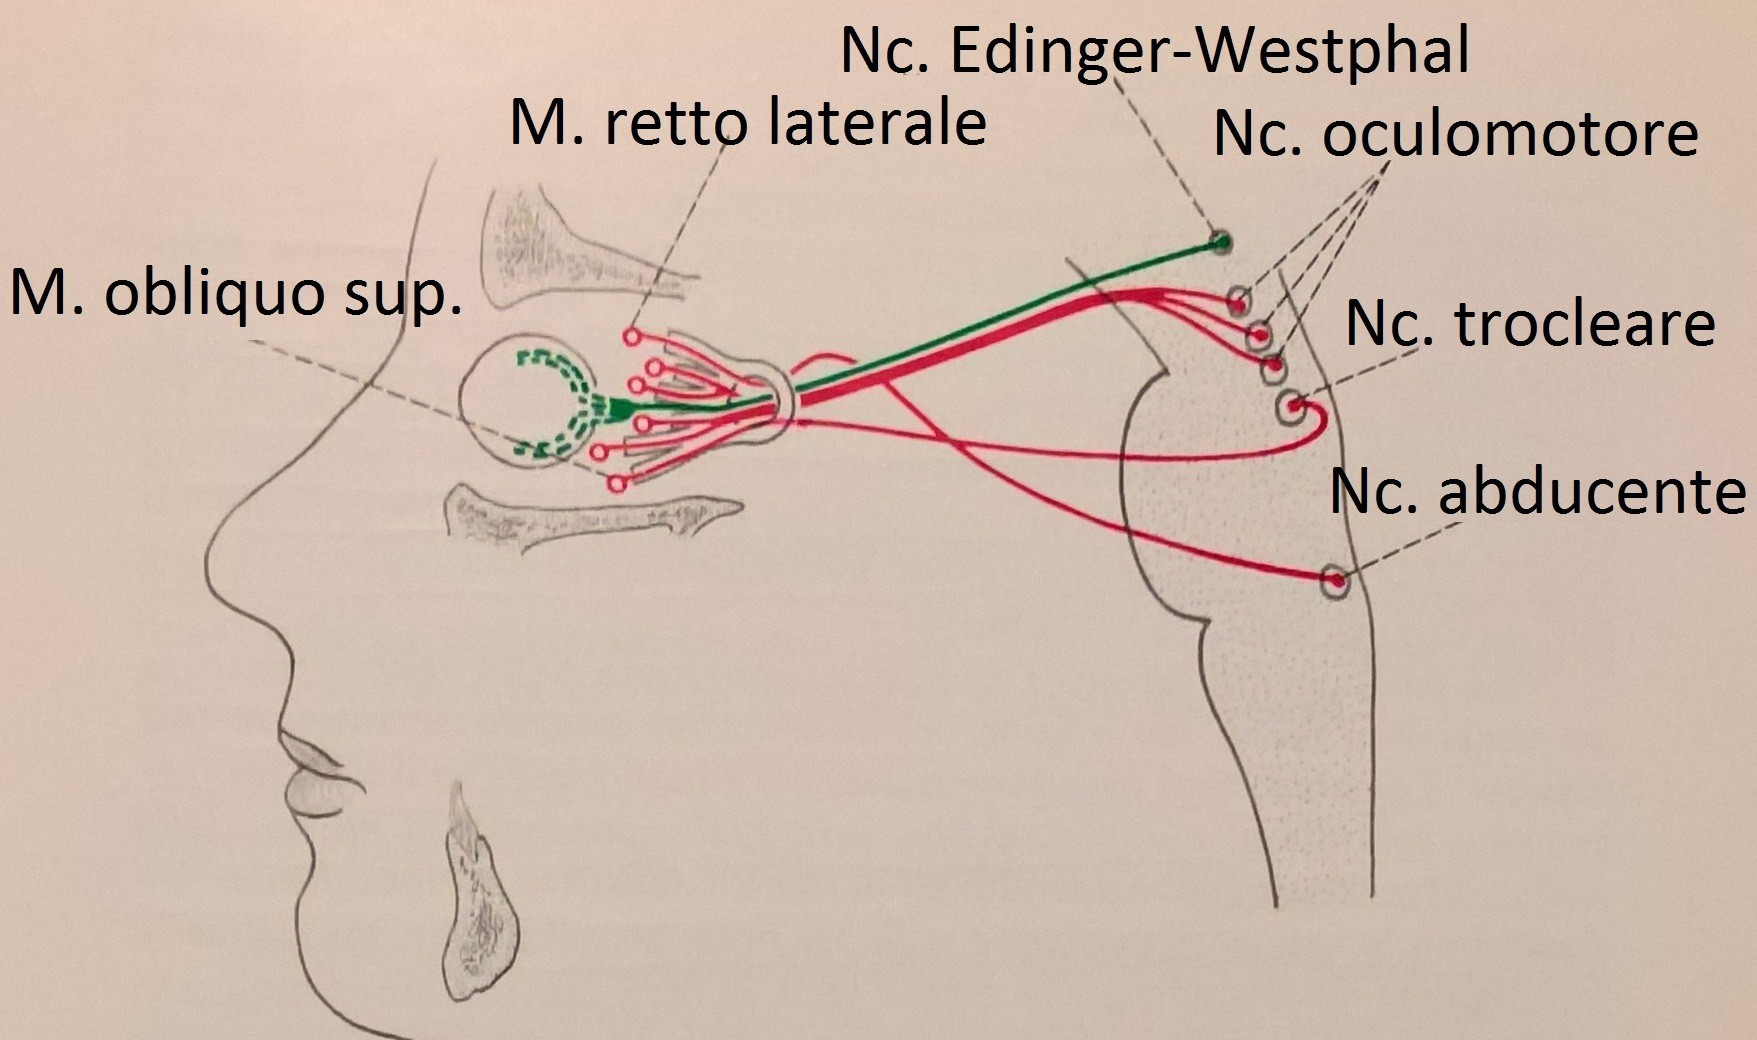
\includegraphics[scale=0.15]{source/immagini/nervo_abducente.jpg}
	\caption[Origine III, IV, VI nervo cranico]{Schema dell'origine e distribuzione dei nervi oculomotore, trocleare, abducente.}
	\label{fig:test10}
\end{figure}
\\\ \\\ 
\textbf{Nervo trigemino (V paio)}: 
\\\ 
(Figura 1.10) Esso è costituito da tre branche: oftalmica, mascellare e mandibolare. Contiene un gran numero di fibre sensitive somatiche e un minor numero di fibre motrici somatiche. La componente sensitiva somatica ha origine dal ganglio semilunare da cui viene inviato un prolungamento periferico nelle tre branche. Grazie a questo le fibre raccolgono stimoli sensitivi estrocettivi della cute della faccia, delle mucose dell’occhio, della bocca, del naso e inoltre stimoli propriocettivi dai muscoli estrinseci dell’occhio, dai muscoli mimici e dagli alveoli dentali. La componente motrice somatica origina dal nucleo masticatorio del trigemino e si distribuisce ai muscoli masticatori, al muscolo del martello, muscolo tensore del velo del palato, muscolo miloioideo e al ventre anteriore del muscolo digastrico. 
Alle tre branche si trovano annessi diversi gangli parasimpatici: ganglio ciliare, ganglio sfenopalatino, gangli sottomandibolare e sottolinguale ed il ganglio ottico. 
Il \emph{nervo oftalmico} nel suo decorso trova il ganglio ciliare, dal quale partono le fibre parasimpatiche che si portano ai musco intrinseci del bulbo oculare. Prima di raggiungere la fessura orbitaria superiore, si divide in nervo nasociliare, nervo frontale e nervo lacrimale.
Il \emph{nervo mascellare} si distribuisce ad un’estesa area cutanea della faccia ed alla mucosa delle cavità nasali e della bocca. È annesso al ganglio sfenopalatino, centro intercalato sul decorso delle fibre parasimpatiche che innervano la ghiandola lacrimale e le ghiandole della mucosa nasale e del palato.
Il \emph{nervo mandibolare} è un nervo misto costituito da fibre motrici somatiche e sensitive somatiche. Innerva i muscoli masticatori con la componente che giunge dal nucleo motore del ponte; con la componente somatosensitiva che origina dal ganglio semilunare si distribuisce alla cute della parte inferiore della faccia ed a parte della mucosa buccale. 

\begin{figure}[h!]
	\centering
	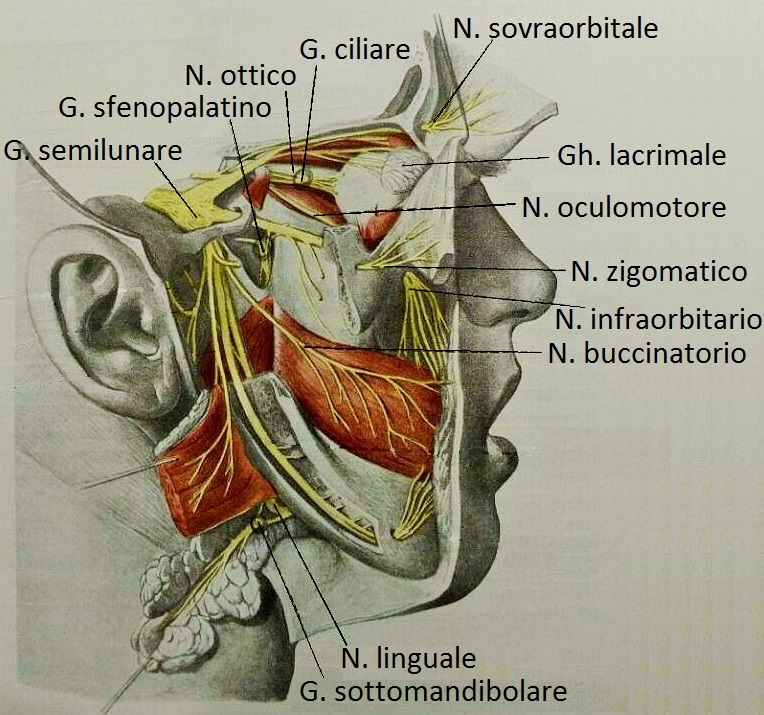
\includegraphics[scale=0.7]{source/immagini/nervo_trigemino.jpg}
	\caption[Nervo trigemino]{Nervo trigemino.}
	\label{fig:test11}
\end{figure}

\section{Funzioni}

\subsection{Stato refreattivo dell'occhio}

Il potere refrattivo dell’occhio può essere considerato la somma di una serie di superfici refrattive, quali la cornea, il cristallino, l’umor acqueo e l’umor vitreo, oppure come la somma delle distanze che separano ogni superficie con differente indice di rifrazione. Dal momento che il potere è determinato dai raggi di curvatura delle superfici e dal loro indice e siccome lo stato refrattivo finale è calcolato dalla relazione del potere refrattivo con la retina, l’ametropia, cioè l’anormale condizione refrattiva dell’occhio, è suddivisa in due categorie:
 \begin{description} 
 \item[assiale:]dipende dalla lunghezza dell’occhio. 
 \item[refrattiva:]dipende dal potere dell’occhio. Il cambiamento del potere dell’occhio può essere dovuto all’indice di rifrazione dei mezzi oppure alla curvatura degli stessi.
Un soggetto è considerato emmetrope quando, guardando all’infinito, il fuoco del sistema di lenti dell’occhio cade sulla retina e perciò l’immagine viene vista a fuoco. Nel caso avvenga una variazione della perfetta coincidenza del fuoco principale dell’occhio con la retina, allora si hanno anomalie rifrattive o errori di rifrazione.
\end{description}
Gli errori rifrattivi si classificano in base a dove cade il fuoco del sistema occhio rispetto alla retina:
 \begin{description}
 \item[miopia:]se il fuoco cade anteriormente alla retina, causato da un occhio con potere maggiore oppure con lunghezza assiale maggiore.
 \item[ipermetropia:]se il fuoco cade posteriormente alla retina, causato da un occhio con potere minore oppure un occhio con lunghezza assiale minore.
 \item[astigmatismo:]se non esiste un fuoco singolo per tutti i meridiani dell’occhio ed è detto miopico se i fuochi cadono prima della retina o ipermetropico se cadono dopo la retina.
\end{description}


\subsection{Accomodazione}

L’accomodazione è il meccanismo che consente di aumentare il potere convergente dell’occhio e quindi di vedere nitidamente gli oggetti a tutte le distanze.
L’accomodazione risulta rilassata in un soggetto emmetrope quando guarda all’infinito, mentre la attiva per guardare a diverse distanze ravvicinate. Usando il massimo potere accomodativo, si ha a fuoco una distanza prossimale che si definisce punto prossimo, ed è la distanza più vicina all’occhio vista ancora nitidamente. Il punto remoto è invece la maggiore distanza che può essere vista nitidamente. La differenza tra punto remoto e punto prossimo è detta estensione accomodativa, mentre la stessa differenza ma espressa in diottrie è detta \emph{ampiezza accomodativa}. L’ampiezza accomodativa è la quantità massima di potere accomodativo o diottrico, che l’occhio può aggiungere partendo da una condizione di emmetropizzazione. Essa viene calcolata facendo il reciproco diottrico del punto prossimo, misurato in metri, con occhio emmetrope o emmetropizzato.

Con il passare degli anni la capacità di variazioni di messa a fuoco dell’occhio subisce una lenta e continua riduzione ed oltre un certo valore assume il nome di presbiopia. Questa è dovuta ad una diminuzione della capacità di modifica della curvatura delle superfici del cristallino, per perdita di elasticità della capsula.
\\\

La variazione accomodativa può essere considerata come una retroazione ad un particolare stimolo, ma può anche essere indotta indirettamente quando vi è un atto di convergenza volontario. Nell’osservazione di un oggetto a distanza prossimale sono diversi i fattori che influenzano l’accomodazione, tra questi: la sfocatura dell’immagine retinica, il movimento dell’oggetto, la sua distanza apparente, la binocularità. Si presume che l’accomodazione sia servita sia dal sistema nervoso simpatico che parasimpatico. Il sistema parasimpatico ha il ruolo principale e le sue fibre pregangliari originano dal nucleo di Edinger-Westphal (Figura 1.11), a livello del mesencefalo in prossimità del nucleo oculomotore, procede con il terzo nervo cranico, raggiungono poi il ganglio ciliare, da dove si dipartono fibre postgangliari che penetrano nell’occhio lungo i nervi ciliari corti, mentre altre fibre viaggiano con i nervi ciliari lunghi. Sul ruolo del sistema simpatico sono presenti delle controversie, ma sembra che i due sistemi abbiano ruolo antagonista, come in tutte le attività autonome, con effetto dominante del parasimpatico nella stimolazione accomodativa ed una funzione di aiuto nel passaggio dal vicino al lontano per il simpatico. Per la componente simpatica che innerva il muscolo ciliare, si sa che origina nel diencefalo e viaggia lungo il midollo spinale fino al più basso segmento cervicale e il più alto segmento toracico, fa sinapsi con il centro cilio-spinale di Budge, nel tratto intermediolaterale del midollo. Da qui i nervi di secondo ordine lasciano il midollo dall’ultima vertebra cervicale e prima toracica; queste fibre preganglionari scorrono e fanno sinapsi con il ganglio cervicale superiore. Le fibre continuano fino al plesso carotideo ed entrano nell’orbita, o con la prima divisione del nervo trigemino (oftalmico), oppure indipendentemente, dove possono unirsi con i nervi ciliari brevi e lunghi.

\begin{figure}[h!]
	\centering
	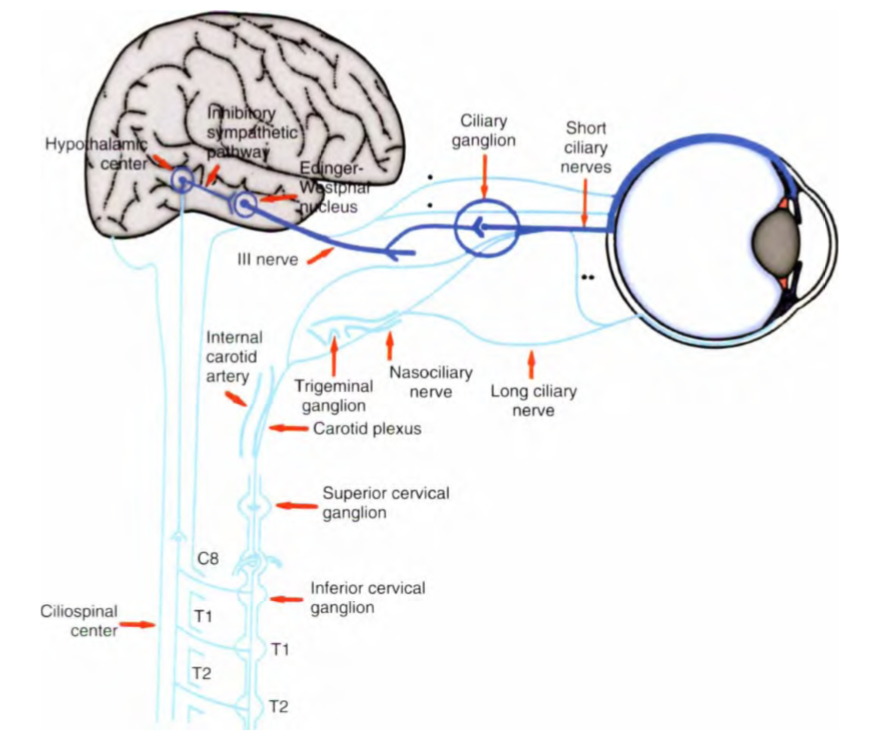
\includegraphics[scale=0.70]{source/immagini/accomodazione.png}
	\caption[Vie parasimpatica e simpatica del muscolo ciliare]{Vie parasimpatica e simpatica del muscolo ciliare.}
	\label{fig:test12}
\end{figure}

La stimolazione dell’accomodazione avviene nella seguente sequenza di eventi:
 \begin{enumerate}
  \itemsep-0.5em 
 \item i coni della retina sono stimolati dall’annebbiamento
 \item la somma dei segnali di annebbiamento viene trasmessa attraverso lo strato magnocellulare del nucleo genicolato laterale alla corteccia visiva
 \item la somma delle risposte delle cellule corticali formula il segnale di annebbiamento
 \item il segnale viene trasmesso anche all’area parieto-temporale e al cervelletto per processare l’informazione
 \item il segnale va al mesencefalo, ai nuclei oculomotori, ai nuclei di Edinger-Westphal dove viene formulato il comando
 \item il comando motore viene trasmesso al muscolo ciliare tramite il nervo oculomotore, il ganglio ciliare e poi i nervi ciliari corti
 \item viene cambiato lo stato di contrazione del muscolo ciliare
 \item il cristallino si deforma per ottenere la messa a fuoco sulla retina dell’immagine e quindi una visione più chiara.
\end{enumerate}

Associata alla risposta accomodativa vi sono i fenomeni della contrazione pupillare e convergenza, che avvengono per sincinesia e costituiscono la reazione al punto prossimo. La risposta accomodativa avviene per un cambio di vergenza della luce a livello retinico in seguito all’avvicinamento dell’oggetto. La miosi è una risposta riflessa e la configurazione del nervo oculomotore suggerisce che le tre funzioni siano collegate. Però la convergenza è solo uno dei fattori che influenzano l’accomodazione, come lo stimolo di convergenza non deriva integralmente dall’accomodazione.

Gli oggetti situati a diverse distanze nello spazio sono percepiti singoli grazie alla capacità degli occhi di mutare il loro allineamento nello spazio. Per ottenere la visione binoculare singola è necessario che le due fovee, che sono i punti retinici corrispondenti, siano allineate sullo stesso oggetto di interesse, per cui si dice che i due occhi convergono sul medesimo oggetto. 
Nell’utilizzo quotidiano degli occhi è necessario che la convergenza e l’accomodazione funzionino in armonia per consentire una nitida visione binoculare singola. Quando gli occhi convergono si ha la stimolazione indotta dell’accomodazione, chiamata accomodazione convergente. Se un occhio o gli occhi accomodano sopravviene una stimolazione della convergenza, che prende il nome di convergenza accomodativa. 

Convergenza e accomodazione, abbiamo detto essere collegate, ma con un certo grado di libertà. Infatti la convergenza continua ad essere funzionante anche in persone presbiti con ridottissima capacità accomodativa, mentre il giovane ipermetrope è abituato ad utilizzare una quantità di accomodazione in eccesso alla quantità utile di convergenza. L’ammontare di accomodazione utilizzabile senza mutamento della convergenza si chiama accomodazione relativa. Allo stesso modo la quantità di convergenza che può variare mantenendo l’accomodazione stabile, è detta convergenza relativa.



\subsection{Fusione e binocularità}

La visione singola, in condizioni binoculari, è permessa dal fatto che per ogni elemento retinico stimolato da uno dei due occhi esiste un corrispondente elemento retinico nell’altro occhio con la stessa localizzazione spaziale. L’elemento retinico è l’insieme delle strutture che elaborano la sensazione visiva in risposta alla stimolazione di un’area unitaria della retina. Ciascun elemento retinico localizza lo stimolo in una determinata direzione detta “direzione visiva della percezione”, e la linea che unisce il punto fissato con la fovea è la linea principale di direzione.

La visione binoculare avviene in due fasi. La prima, la visione monoculare simultanea, è dovuta alla stimolazione visiva dei due occhi. La seconda è la fusione delle due percezioni monoculari in una percezione singola a livello della corteccia occipitale.

Ciascun recettore retinico ha nell’altra retina un corrispondente recettore con la stessa localizzazione spaziale. Punti retinici con la stessa localizzazione spaziale sono detti “punti retinici corrispondenti”. La corrispondenza retinica spiega la visione binoculare singola, cioè la fusione sensoriale, che è un complesso meccanismo fisiologico attraverso il quale le immagini che colpiscono le due retine in punti corrispondenti, dopo essere giunte alla corteccia visiva, vengono percepite come un’unica immagine che rappresenta la fusione delle due immagini primitive. La superficie immaginaria nello spazio composta da tutti i punti le cui immagini cadono su punti retinici corrispondenti è detta oroptero. La fusione può avvenire anche in caso l’immagine non colpisca la retina in punti retinici perfettamente corrispondenti, l’importante è che si trovino all’interno dell’area di panum, l’area intorno all’oroptero in cui possono trovarsi gli oggetti per essere visti singoli. La disparità tra le immagini che vengono fuse entro i limiti dell’area di panum costituisce la base fisiologica per la percezione della stereopsi.

\\\ \\\
\textbf{Stereopsi}
\\\
La stereopsi è la capacità di fondere immagini leggermente differenti percepite da ciascun occhio durante l’osservazione di un oggetto tridimensionale. La fusione avviene se vengono stimolati punti retinici corrispondenti o con piccole disparità, in modo che non creino diplopia. La fusione può essere motoria o sensoriale, la prima porta a un aggiustamento della posizione dei due occhi per centrarsi sul punto di fissazione, mentre la seconda è un’integrazione mentale dei segnali provenienti dai due occhi. Per mantenere la fusione sensoriale è necessario che i due occhi siano sempre bene allineati e che le loro direzioni visive principali si incontrino nel punto di fissazione, se non dovesse succedere avverrebbe la diplopia.
\\\
Per osservare gli oggetti a diverse distanze si effettuano movimenti coordinati degli occhi che possono essere volontari o riflessi. Gli occhi possono compiere movimenti coniugati (versioni) dove ruotano nella stessa direzione e con la stessa ampiezza, oppure non coniugati (vergenze) dove si muovono in direzione opposta per spostare nello spazio il punto di intersezione degli assi visivi. Quando avvciiniamo un oggetto lontano, avviene il fenomeno della convergenza. Essa può essere misurata in diottrie prismatiche, che è quella quantità di prisma in grado di determinare lo spostamento del raggio di luce di 1 cm alla distanza di 1 m. 
\\\
Come detto prima, l’accomodazione e la convergenza interagiscono. Può avvenire la risposta in convergenza prodotta da un’unità di stimolo accomodativo e può essere espressa tramite il rapporto convergenza accomodativa/accomodazione (AC/A), che misura la capacità di risposta della funzione di convergenza alla stimolazione di una unità di accomodazione. L’accomodazione e la convergenza sono controllate da due sistemi differenti: autonomo per l’accomodazione e volontario o scheletrico per la convergenza. Per avere una visione binoculare efficiente queste due componenti devono funzionare in armonia.
\\\ \\\
\textbf{Eteroforie}
\\\
La visione binoculare può essere mantenuta in presenza di una perfetta coordinazione dell’apparato neuromuscolare dei due occhi, però essendo un sistema complicato, raramente si ha questa condizione. Anche in assenza di una adeguata centratura, però, è possibile mantenere gli occhi allineati sull’oggetto grazie ai riflessi fusionali compensatori. Le condizioni che ne richiedono l’uso sono le “eteroforie o strabismo latente”, se il riflesso è assente, allora si ha “strabismo manifesto”, se si presenta saltuariamente allora si ha “strabismo intermittente o tropia”. Le forie possono essere di tre tipi in base alla direzione della deviazione:
 \begin{description}
 \item[ortoforia:]quando gli occhi sono centrati senza l’utilizzo di sforzi fusionali
 \item[exoforia:]quando, interrompendo la fusione con un mezzo dissociatore, gli occhi non rimangono allineati al punto di fissazione, ma uno devia verso la tempia
 \item[esoforia:]quando gli occhi, in condizione di dissociazione, deviano verso il naso
\end{description}
\\\ \\\
\textbf{Disparità di fissazione}
\\\
Si è detto che la fusione può avvenire per punti retinici disparati, a patto che si trovino nell’area di Panum. In caso di eteroforia le immagini possono non stimolare esattamente le due fovee, ma la disparità può essere lieve e gli occhi possono deviare solo di un’entità pari alla disparità di fissazione. La disparità di fissazione è una condizione presente in eteroforici con visione binoculare singola, rappresenta quindi l’ammontare di slittamento retinico consentito all’eteroforico nel limite della visione binoculare.
\chapter{La postura e ciò che la influenza}

La posturologia studia l’essere umano nel suo ambiente vitale ed è la prima a servirsi dei riflessi posturali per l’analisi di patologie funzionali. La postura è definita come “il modo di stare in equilibrio nelle varie posizioni”, ed esprime una funzione relativa ai modi e alle capacità del corpo umano di acquisire e mantenere tutte le posizioni, conservando l’equilibrio. 

Il sistema dell’equilibrio può essere considerato un sistema complesso e aperto: complesso perché costituito da un insieme di sottoinsiemi reciprocamente interrelazionati, aperto perché ciascuno di essi interagisce con l’ambiente e con la situazione in atto. Ogni componente del sistema è in rapporto con tutte le altre parti che lo costituiscono e va incontro a modificazioni, conseguentemente alle variazioni di queste ultime, al fine di costruire un insieme funzionale stabile. 

Il sistema che regola la staticità del corpo nello spazio è il sistema tonico posturale. Il Sistema-Tonico-Posturale (STP) è un sistema cibernetico, un circuito che necessita di un’afferenza (input), proveniente dagli esterocettori e propriocettori, di centri superiori di modulazione, integrazione, pianificazione, risposta, controllo e di un’efferenza (output) che traduce il segnale elaborato dai centri superiori in gesto motorio (Schema in Figura 2.1). Il suo studio consente di discriminare al meglio fra gli elementi determinanti la causa primaria di una sindrome patologica. 
\\\ \\\ \\\ \\\ \\\ \\\ \\\
Le strutture recettoriali concorrono nell’apportare informazioni posturali, che, una volta elaborate, migliorano l’equilibrio muscolare. Queste sono:

 \begin{itemize}
 \itemsep-0.6em 
 \item[--]sistema visivo: la formazione dell’immagine retinica fornisce all’individuo informazioni relative ai suoi movimenti nello spazio. I recettori visivi sono i coni e i bastoncelli che informano sulla situazione ambientale
 \item[--]apparato stomatognatico
 \item[--]sistema vestibolare: endolinfa e otoliti dell’orecchio interno determinano importanti adeguamenti del sistema posturale in relazione alle tre dimensioni dello spazio, da coordinare/integrare con le informazioni provenienti dagli apparati descritti precedentemente
 \item[--]recettori presenti sulla cute della pianta del piede
 \end{itemize}
 
 Il sistema posturale funziona come un insieme che ha lo scopo di lottare contro la forza di gravità per mantenere la posizione eretta equilibrando e coordinando le funzioni a seconda del fine. Ciascun recettore apporta le proprie specifiche informazioni che poi, rielaborate e integrate, daranno luogo allo schema posturale finale. Per realizzare queste funzioni neurofisiologiche, l’organismo utilizza informazioni provenienti sia dall’esterno (esterocettori: sensibili al tocco, alla pressione e al movimento) che dall’interno (enterocettori, propriocettori: danno informazioni sulle risposte statiche e dinamiche dei muscoli e sulle tensioni esercitate sui tendini)\cite{bib6}.
 \\\ \\\
 \begin{figure}[h!]
	\centering
	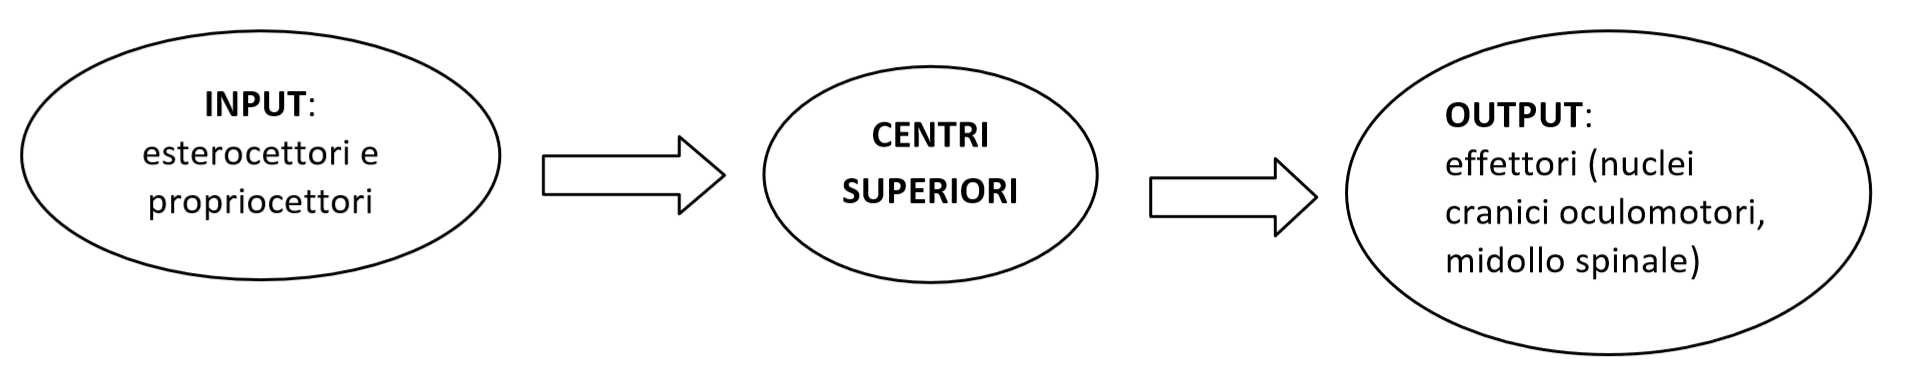
\includegraphics[scale=0.4]{source/immagini/STP.png}
	\caption[Schema del STP, passaggi dell'elaborazione dell'informazione]{Schema del STP, passaggi dell'elaborazione dell'informazione.}
	\label{fig:issuexample}
\end{figure}

\\\ \\\ \\\
\section{L'apparato stomatognatico}

Il complesso stomatognatico svolge funzioni come la masticazione, la deglutizione, la fonazione, la digestione e la respirazione\cite{bib6}. Esso è formato da:
\begin{itemize}
 \itemsep-0.5em 
 \item[--]una struttura ossea costituita dalle ossa mascellari e palatine, dalla mandibola, dall’articolazione temporo-mandibolare (ATM) e dalle arcate dentarie.
 \item[--]da una struttura miofasciale, costituita  dai muscoli masticatori e dai muscoli di contrappoggio della masticazione (trapezio, sternocleidomastoideo, sopra e sotto-ioidei)
 \item[--]strutture legamentose
 \item[--]innervazione sensitivo-motoria e neuro-vegetativa
 \item[--]organo della lingua.
 \end{itemize}
 
L’organo della lingua (Figura 2.2) merita un approfondimento, poiché fornisce numerose informazioni posturali. Esso è costituito da una porzione anteriore (corpo) ed una posteriore (base), e dal frenulo linguale che collega la superficie ventrale della lingua con il pavimento del cavo orale, in corrispondenza della linea mediana. Nel corpo linguale si distingue l’apice (punta), una faccia superiore (dorso), una inferiore e due bordi laterali. I muscoli estrinseci (Figura 2.3) presenti nella lingua sono: genioglosso (protusore), ioglosso (abbassatore, retrattore), stiloglosso (elevatore e retrattore), palatoglosso (elevatore del corpo), faringoglosso e condroglosso. I muscoli intrinseci sono composti da sistemi di fascetti muscolari detti longitudinali superiore e inferiore, trasversale e verticale. I muscoli intrinseci regolano la forma, mentre gli estrinseci determinano la posizione. 

L’innervazione motoria della lingua è data dal nervo ipoglosso, mentre quella sensitiva dal ramo linguale del nervo trigemino per i due terzi anteriori, dal glossofaringeo per la base e dal nervo laringeo superiore del nervo vago per la zona glossoepiglottica. 

La lingua è coinvolta nelle attività di masticazione, deglutizione e fonazione. Vi sono dei recettori che permettono di controllare la postura della lingua, questi sono: corpuscoli di Meckel, di Pacini, di Meissner, di Ruffini e i propriocettori. La capacità di riconoscere la posizione della lingua e delle strutture anatomiche circostanti, dipende dalle afferenze sensoriali\cite{bib20}.

\begin{figure}[h!]- 
\centering
\begin{minipage}{.36\textwidth}
  \centering
  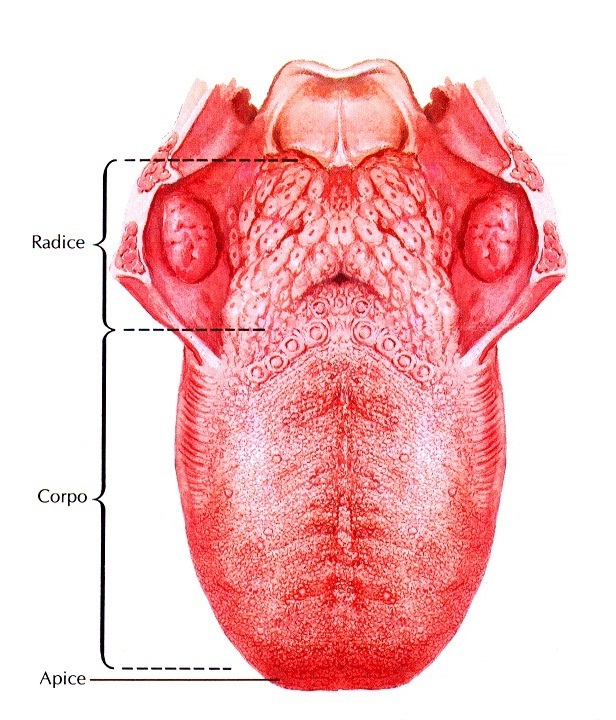
\includegraphics[scale=0.30]{source/immagini/lingua_anatomia.jpg}
  \captionof{figure}{Struttura della lingua.}
  \label{fig:test1}
\end{minipage}%
\begin{minipage}{.5\textwidth}
  \centering
  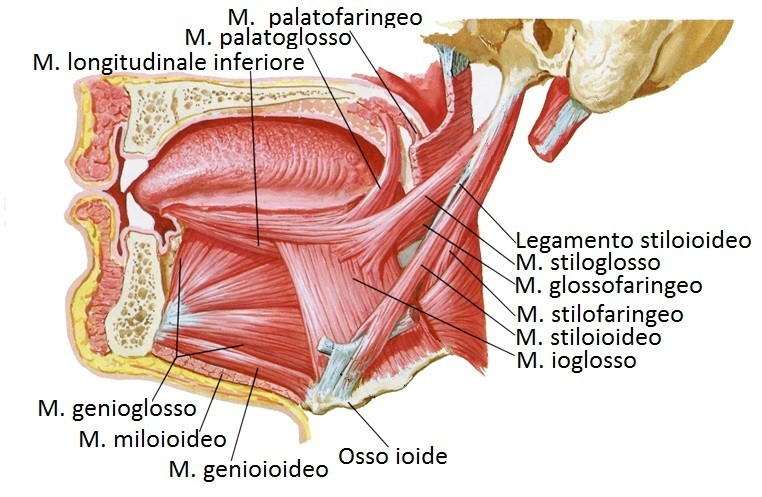
\includegraphics[scale=0.33]{source/immagini/muscoli_estrinseci_lingua.jpg}
  \captionof{figure}{Muscoli estrinseci della lingua.}
  \label{fig:test2}
\end{minipage}
\end{figure}
\\\ \\\ \\\ \\\
Dagli studi di Ferrante\footnote{Dott. Antonio Ferrante: L'importanza della deglutizione nell'ambito gnatologico e posturale (www.ortodonzia.net/deglutizione)}, emerge che, in condizioni fisiologiche, la lingua a riposo deve essere posizionata con l'apice a contatto del palato, subito dietro la papilla retroincisiva, punto corrispondente allo spot linguale, ossia all'emergenza della seconda branca trigeminale dal foro naso-palatino.  Lo spot è situato precisamente tra la papilla interdentale, che si trova nella parte mediana del palato duro, subito dietro gli incisivi superiori, e la prima ruga palatina (Figura 2.4). Di fondamentale importanza per la definizione dello spot e del suo ruolo, sono gli studi di Halata e Baumann (1999)\footnote{Halata Z e Baumann KI, Sensory nerve endings in the hard palate and papilla incisiva of the rhesus monkey, ANAT
EMBRYO, 199(5), 1999, pp. 427-437}, in cui viene indagata l'innervazione sensitiva del palato duro nel macaco Rhesus, dimostrando che nel punto comunemente chiamato \emph{spot palatino} è presente una quantità elevatissima di cinque diversi esterocettori. 

La postura linguale e la compressione dello spot ad ogni atto deglutitorio comportano la stimolazione dei recettori naso-palatini che continuano ad informare il quinto paio dei nervi cranici. La stimolazione dello spot risulta, quindi, di fondamentale importanza anche durante la funzione deglutitoria. Durante la fase orale della deglutizione i denti vengono a contatto tra loro (massima intercuspidazione) grazie ai muscoli masseteri e temporali, la lingua prende progressivamente contatto con il palato duro a partire dallo spot con movimento antero-posteriore. Il contatto in massima intercuspidazione tra le arcate dentarie durante la fase deglutitoria appena descritta risulta di notevole importanza, perché ciò permette di conferire grande stabilità alla mandibola e, di conseguenza, la lingua avrà la possibilità di compiere un movimento identico e ripetibile, permettendo alla deglutizione di generare un input meccanico e neurologico sempre uguale.

 \begin{figure}[h!]
	\centering
	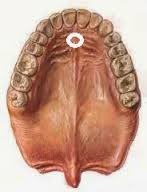
\includegraphics[scale=0.4]{source/immagini/spot_palatino.jpg}
	\caption[Lo spot palatino]{Lo spot palatino.}
	\label{fig:issuexample}
\end{figure}

Tutti gli elementi elencati precedentemente condizionano l’occlusione, cioè il rapporto tra denti superiori e inferiori, i quali dovrebbero cooperare perfettamente. Ciò non avviene quando vi sono delle disfunzioni derivanti da traumi diretti o a distanza che possono creare condizioni che disturbano l’equilibrio della struttura e della funzione stomatognatica con ripercussione neuro-muscolare locale o posturale. L’apparato stomatognatico è anche un recettore posturale, cioè un organo che invia le informazioni al cervello su come interpretare lo spazio. 

Numerose ricerche cliniche dimostrano come un disturbo dell’equilibrio occlusale si ripercuota verso l’insieme del sistema posturale, e viceversa. 
L’apparato stomatognatico presenta infatti molti recettori:
\begin{itemize}
 \itemsep-0.5em 
 \item[--]meccanocettori capsulari, presenti soprattutto nella zona posteriore della capsula. La loro scarica al sistema nervoso centrale permette l’attivazione dei muscoli della mandibola che ne riadattano la postura in base all’informazione inviata. Con il tempo, questo meccanismo cronico provocherà disfunzioni che coinvolgono muscoli di contro-appoggio come trapezio e sternocleidomastoideo, i quali funzionano in sinergia con l’occhio.
 \item[--]recettori muscolari
 \item[--]recettori dentali che sono in grado di rispondere a stimoli infinitesimali. In caso di disfunzione patologica le risposte del sistema nervoso centrale coinvolgono non solo i muscoli dell’apparato stomatognatico, ma anche la muscolatura degli altri distretti come lingua, testa, colonna cervicale.
\end{itemize}
 
\\\ \\\
\section{Influenza dell’occhio e dell’apparato stomatognatico sulla postura}
 
Disfunzioni all’apparato stomatognatico o al sistema visivo possono creare perturbazioni al sistema posturale, costringendolo a riadattarsi. 

La struttura dell’occhio è deputata alla conversione dell’immagine. La possibilità di correzione è relativa, abbastanza limitata e dipende dalle possibilità adattative di messa a fuoco. Questa funzione dipende da: forma dell’occhio, elasticità e trasparenza del cristallino. Riguardo la funzione oculomotoria, l’occhio, grazie alla muscolatura estrinseca, può essere allungato, stirato e compresso da un’alterata azione di questi muscoli. A causa di questi cambiamenti possono verificarsi difetti nella convergenza o alterazioni nella sovrapposizione delle immagini. Quindi fra le disfunzioni oculari che possono intervenire nel determinare uno squilibrio tonico posturale si riconoscono: disturbi di rifrazione, disturbi di convergenza  ed eteroforie. In particolare i disturbi di convergenza e del parallelismo determinano delle necessità di integrazione dello schema corporeo, il quale dovrà scegliere uno schema alternativo a quello ottimale. Il fatto di avere un’eccellente visione non esclude che possa esservi il difetto di convergenza o parallelismo\cite{bib6}.

La relazione tra sistema visivo e postura nasce dalla prima volta che il bambino solleva la testa e comincia ad osservare ciò che lo circonda. Il perfezionamento del sistema visivo porta al raddrizzamento della posizione della testa, abituandola ad una posizione verticale. Successivamente il sistema vestibolare comincia a migliorare la coordinazione e lo spostamento del capo in diverse posizioni. Questo porta all’acquisizione di diverse esperienze visive le quali vengono integrate con gli altri sistemi. In seguito il sistema visivo ambientale continua ad orientare il corpo nello spazio mentre il sistema visivo focale sviluppa le capacità necessarie per organizzare forme complesse, che saranno necessarie per la lettura. Movimenti oculari ottimali dipendono dalla stabilità del collo, del tronco e dalla mobilità della testa che permettono di trovare il centro di gravità per muoversi nello spazio. Perciò se dovessero verificarsi delle alterazioni delle funzioni visive, il corpo si adatterebbe di conseguenza alle nuove informazioni che riceve, assumendo una postura alterata\cite{bib8}.
\\\

L’apparato stomatognatico, come precedentemente descritto, è caratterizzato da diverse strutture che agiscono in armonia per svolgere differenti funzioni (parlare, masticare, deglutire). In particolare l’articolazione temporomandibolare (ATM) contrae connessioni muscolari e lagamentose con la regione cervicale, creando un complesso funzionale chiamato sistema cranio-cervico-mandibolare. Il sistema stomatognatico è connesso alla postura grazie all’esistenza delle catene muscolo-fasciali. La fascia è il tessuto connettivo fibroso che, organizzato in foglietti e setti, separa ed unisce ogni parte del corpo. Essa presenta anche una contrattilità autonoma che influenza la postura dell’intero corpo a causa del pretensionamento della catena miofasciale. La catena miofasciale è un gruppo di muscoli interconnessi attraverso la fascia. La sua esistenza può spiegare perchè disordini di funzioni muscolari come masticazione e deglutizione possono essere trasmesse a distanza nel corpo umano. Sempre per questo alterazioni funzionali di una parte del corpo possono creare disordini in un’altra\cite{bib20}. 

Oltre alla catena miofasciale esiste una via detta oculocefalogira, costituita dalle connessioni neurologiche tra i sistemi. Infatti sono presenti numerose connessioni anatomiche tra i sistemi connessi al trigemino (sistemi trigeminali) e le strutture nervose coinvolte nel mantenimento della postura. I nuclei mesencefalici del trigemino, come visto nel capitolo 1, connettono i neuroni anche esternamente al sistema nervoso centrale e quindi questo spiega il motivo per cui i soggetti con disfunzioni stomatognatiche presentano stimoli in diversi distretti del corpo. Inoltre studi rivelano che esistono connessioni tra il nucleo principale del trigemino e il nucleo vestibolare e preposito dell’ipoglosso. Quest’ultimo è anche un importante centro nervoso per il controllo della posizione e movimento degli occhi, dovuto alla sua stretta relazione con il nucleo vestibolare, il cervelletto e il nucleo oculomotore.
\\\
Altri studi dimostrano la relazione tra l’occlusione dentale, il sistema oculomotore e la stabilità visiva. Monaco ed al. hanno rilevato una maggiore presenza di difetti di convergenza sia in soggetti adulti che presentavano una disfunzione temporo-mandibolare, con dolore miofasciale e all’area del collo e della spalla che in bambini con deviazioni mandibolari laterali. È stato affermato che vi era una maggiore alterazione della funzione binoculare nei soggetti che presentavano queste disfunzioni, piuttosto che nei soggetti sani\cite{bib5}.  
\\\

Tutte queste connessioni anatomiche suggeriscono che questa porzione di sistemi trigeminali influenza fortemente la coordinazione, la postura e la vista. Sembra che le informazioni sensoriali ricevute dai recettori del sistema stomatognatico vengano integrate con le informazioni  provenienti dai sistemi vestibolare e oculomotore. Le modifiche delle stimolazioni trigeminali possono quindi causare uno sbilanciamento dei sistemi vestibolare ed oculomotore.


\subsection{Ripercussioni dello SMOF sul sistema visivo}
 
Definiamo lo Squilibrio Muscolare Oro-Facciale (SMOF) come un’alterazione dell’equilibrio delle strutture del complesso bucco-facciale, quindi dell’apparato stomatognatico, che può essere causata da:

\begin{itemize}
 \itemsep-0.5em 
 \item[--]mancato passaggio dalla deglutizione infantile a quella adulta con la corretta postura linguale e quindi corretta deglutizione
 \item[--]malocclusioni dentali
 \item[--]respirazione orale, a causa di patologie o di allergie
 \item[--]scorretta postura della lingua determinata da vizi orali (succhiamento del pollice, prolungato uso del ciuccio o biberon..)
 \item[--]traumi o ferite al complesso oro-facciale
 \item[--]disfunzioni del sistema nervoso centrale\cite{bib22}
\end{itemize}
Le conseguenze dello SMOF e in particolare della funzione deglutitoria si ripercuotono sia sulla postura che su altri distretti corporei. La deglutizione, attraverso la stimolazione trigeminale, può interferire con i recettori posturali principali, tra cui l’occhio. Il motivo per cui i recettori occhio e bocca si influenzano reciprocamente è descritto dalla via \emph{oculocefalogira}. Essa è costituita da:
\begin{itemize}
 \itemsep-0.5em 
 \item[--]una via ascendente, che trasporta le informazioni propriocettive dai recettori paradontali delle arcate superiori e dai recettori dello spot palatino al nucleo mesencefalico del trigemino e da qui proietta ai nuclei del III, IV, VI nervo cranico
 \item[--]una via discendente, dove le afferenze provenienti dall’apparato stomatognatico, proiettano le informazioni al nucleo mesencefalico del trigemino, il quale comunica con il nucleo accessorio spinale, nelle corna anteriori del midollo cervicale (C1-C5). Da qui parte il nervo accessorio (XI) che innerva il muscolo trapezio superiore e lo SCOM (sterno-cleido-occipito-mastideo). Inoltre dai muscoli oculomotori partono fibre che arrivano ai nuclei oculomotori e poi raggiungono il nucleo del trigemino, il quale è coinvolto anche nell’apertura e chiusura della mandibola e nella masticazione\cite{bib25}.
\end{itemize}
\\\
Un disturbo visivo (foria, insufficienza accomodativa, ipoconvergenza, ecc..) può influenzare l’occlusione dentale attraverso variazioni della posizione della testa mediate dal sistema oculocefalogiro ed atte al compenso funzionale del difetto. Però è vero anche che una malocclusione o una deglutizione atipica può determinare una posizione viziata della testa, quindi il sistema visivo dovrebbe adattarsi alla nuova posizione e modificherebbe il suoi parametri. Quindi sebbene l’apparato stomatognatico e il sistema visivo siano funzionalmente distinti, esiste una correlazione sia a livello neurofisiologico, per la comunicazione dei nervi trigemino, oculomotore e accessorio (via oculocefalogira), sia a livello neuromuscolare, per le catene muscolo-connettivali (catene miofasciali).

\chapter{Ricerca}
\section{Ricerca e protocollo}

L’interesse per le relazioni tra occhio, postura e apparato stomatognatico sta crescendo, come dimostra la letteratura
scientifica dell’ultimo decennio e l’approccio dei clinici a riguardo. In particolare le ricerche riportano la presenza di
un’associazione clinica tra le malocclusioni dentali e i difetti di convergenza, come descritto da Silverstrini-Biavati et al. 9
Bilello et al. hanno condotto uno studio che ha portato a verificare la correlazione tra sistema stomatognatico e
oculomotore, notando la presenza di eteroforie o eterotropie e difetti di convergenza in persone con malocclusioni
dentali 10 . Un’altra ricerca condotta da Monaco ed al. suggerisce la correlazione tra difetti di refrazione e malocclusioni,
in particolare: l’incidenza di astigmatismo e ipermetropia è maggiore in soggetti con prima classe dentaria, mentre la
miopia è maggiore per soggetti con seconda classe 11 .

In seguito alla lettura di questi studi e all’approfondimento delle connessioni nervose presenti tra i due sistemi, è nata l’idea di questa ricerca. Essa propone di verificare il cambiamento del sistema visivo in seguito al trattamento logopedico e osteopatico dell’apparato stomatognatico in soggetti con disfunzioni primarie orofacciali. Ciò che si vuole verificare è che la riabilitazione delle disfunzioni orofacciali porti a un miglioramento dei difetti visivi della persona. 
Per difetto visivo si intende: anomalie refrattive, accomodative, muscolari, di convergenza e stabilità. Lo svolgimento della ricerca è stato effettuato a Brescia presso il negozio di ottica Ottico Bertella e in collaborazione con l’ambulatorio della Dottoressa Alice Delbono (logopedista) e il Dottor Stefano Grassotti (osteopata, fisioterapista), nei mesi da settembre 2016 a gennaio 2017. Sono stati coinvolti tutti i soggetti affluenti presso l’ambulatorio e i conoscenti della laureanda e dei collaboratori, per un totale di 93 persone. Tra questi sono stati selezionati complessivamente 19 soggetti che rispettavano i criteri di inclusione e che si sono rivelati disponibili alla partecipazione e all’impegno. Questi sono stati divisi in un gruppo sperimentale e un gruppo di controllo in base alle scelte dei singoli: chi era disposto a sottoporsi al trattamento per la durata di 3 mesi, allora è stato inserito nel gruppo sperimentale, mentre chi ha preferito non impegnarsi nel trattamento ma ha voluto lo stesso essere incluso nella ricerca, allora è stato inserito nel gruppo di controllo.

\section{Materiali e metodi}

Sono stati selezionati 19 soggetti con primarietà deglutitoria e squilibrio muscolare oro-facciale di età media di 25 anni:
10 appartenenti al gruppo sperimentale, 9 appartenenti al gruppo di controllo. Sono stati esclusi:
\begin{itemize}
 \itemsep-0.5em
 \item[--]Soggetti con terapia logopedica per la rieducazione della deglutizione in corso
 \item[--]Soggetti con malattie neurodegenerative
 \item[--]Soggetti non collaboranti (deficit cognitivi, bambini sotto i 6 anni)
\end{itemize}
Entrambi i gruppi sono stati sottoposti ad una valutazione osteopatica-posturale iniziale, dove si è risaliti alla
disfunzione primaria linguale e deglutitoria. Si parla di disfunzione primaria linguale e deglutitoria quando l’alterazione
della funzione linguale genera la disfunzione di altri recettori del STP a cascata, per motivi prevalentemente neurologici
(connessioni tra nuclei della base dei diversi nervi cranici, in particolare III, IV, V, VI, XI nervi cranici).

Successivamente ciascun soggetto è stato valutato dal punto di vista optometrico. La valutazione è stata ripetuta a
distanza di tre mesi per il gruppo di controllo e prima e dopo il trattamento logopedico-osteopatico di tre mesi per il
gruppo sperimentale. Essa comprendeva i seguenti test:

\begin{itemize}
 \itemsep-0.5em
 \item[--]Refrazione
 \item[--]Stereopsi lontano e vicino
 \item[--]Foria ambientale lontano, con Facchin Card
 \item[--]Punto prossimo di convergenza effettuato nelle posizioni: diritto, basso e alto
 \item[--]Foria ambientale da vicino con il metodo di Howell, effettuato nelle posizioni: diritto, basso, alto
 \item[--]Cover test nelle 9 posizioni di sguardo con quantificazione con prismi
 \item[--]Ampiezza accomodativa tramite metodo push up
 \item[--]Disparità di fissazione con Wesson Card
 \item[--]MEM
 \end{itemize}
 

\subsection{Svolgimento della ricerca}

\subsubsection{Test posturali per stabilire primarietà linguale}
\\\
I test posturali esplorano i riflessi neurofisiologici del STP e permettono di ottenere informazioni sul cambiamento
della postura, della simmetria del tono e della forza muscolare, stimolando o inibendo l’attività dei recettori posturali.
A seguito della stimolazione o inibizione può verificarsi il miglioramento o peggioramento della funzione indagata (per
esempio della simmetria del tono muscolare) a seconda di quale recettore viene considerato.

Nella ricerca sono stati utilizzati diversi test posturali, tra cui il “test degli indici” che “studia le simmetrie del tono
muscolare attraverso modificazioni delle informazioni recettoriali” 12 Si inizia proponendo il test di base posizionando il
soggetto in stazione eretta con denti non a contatto e piedi in posizione neutra. Si chiede quindi di anteporre gli arti
superiori con gli indici in avanti. L’arto più indietreggiato segnala un aumento omolaterale del tono dei muscoli
estensori della colonna vertebrale. Dopo aver eseguito il test di base si verifica l’adattamento fra i diversi recettori e il
sistema tonico posturale in vari modi, ad esempio:
\begin{itemize}
 \itemsep-0.5em
 \item[--]si chiede di guardare a destra e a sinistra per attivare la muscolatura estrinseca oculare e il sistema oculogiro. In
fisiologia eseguendo questo test si ha un aumento del tono muscolare contro laterale con arretramento dell’arto. Ad
esempio: la rotazione degli occhi a sinistra fa aumentare il tono dei muscoli estensori di destra, quindi arretra l’arto
superiore di destra. Se ciò non avviene si rileva un problema di oculomotricità non adattato dal STP, quindi il risultato
del test si definisce positivo.
 \item[--]si chiede al soggetto di protrudere la lingua e di deviarla a destra e a sinistra per valutare la risposta del STP rispetto al
recettore linguale. Ad esempio se in un soggetto, quando protrude la lingua, il test di base risulta modificato significa
che vi è una probabile disfunzione linguale che interferisce sul STP, quindi il risultato del test è positivo.
\end{itemize}

Al termine della valutazione si possono osservare diversi risultati positivi, ad esempio in un soggetto si può trovare una
positività sia al test del sistema oculogiro che al test del recettore linguale. Diventa necessario quindi stabilire quale sia
il recettore che interferisce maggiormente con il STP (disfunzione primaria) e che porta in disfunzione anche l’altro
recettore (disfunzione secondaria).

Un recettore risulta primario se, dopo averlo stimolato, porta ad un miglioramento degli altri recettori. Ad esempio se
si ha sia positività del recettore oculare sia positività del recettore linguale si può effettuare uno stretching della lingua
e, in seguito, verificare con il test degli indici se i test descritti sopra sono diventati negativi. Se ciò avviene si ha una
primarietà linguale e la disfunzione del recettore oculare risulta secondaria alla disfunzione linguale. Se invece dopo lo
stretching linguale il test sul recettore linguale risulta negativo a occhi chiusi mentre positivo ad occhi aperti, allora la
disfunzione del recettore oculare è primaria sulla disfunzione linguale.
\\\ \\\
\subsubsection{Test per visita optometrica}
\\\ 
Per tutti i test, eccetto la refrazione, è stato utilizzato l’eventuale occhiale che sarebbe stato indossato durante il
periodo di trattamento. Laddove il soggetto avesse cambiato correzione senza preavviso, i test pre e post trattamento
sono stati effettuati con le stesse lenti. Inoltre è stato valutato il grado di fatica (da 1 che indica assenza di fatica a 5 che
indica molta fatica) provato durante lo svolgimento di ogni test.
\\\ \\\
\textbf{Refrazione:} la refrazione è stata effettuata tramite il metodo della sospensione foveale, laddove il soggetto non
presentava fastidi. In alternativa è stato effettuato il test #7 con il forottero. Il risultato riportato è dato dalla lente che
permettesse la migliore acutezza visiva e il migliore bilanciamento binoculare per il soggetto.
\\\ \\\
\textbf{Stereopsi:} è stato utilizzato per vicino il test della mosca di Titmus (Figura 3.1) a 40 cm, in particolare si fa riferimento al test con
cerchi per la percezione della profondità (da 800 a 40 sec).

\begin{figure}[h!]
	\centering
	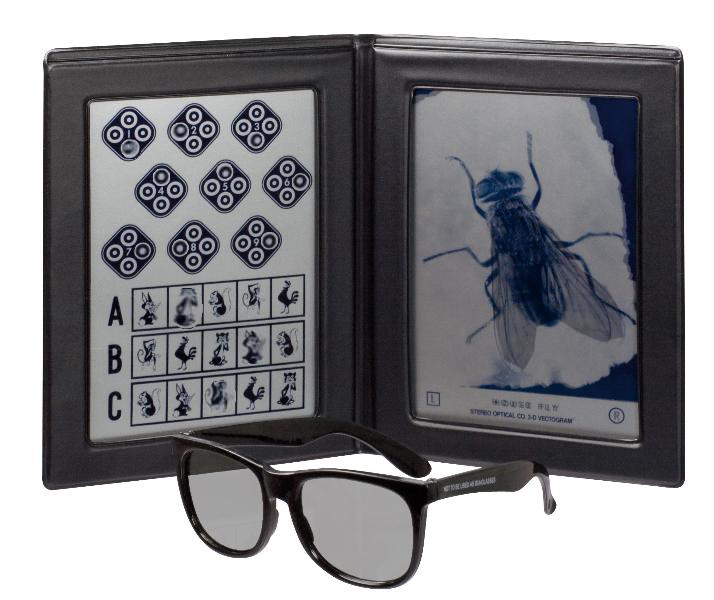
\includegraphics[scale=0.22]{source/immagini/titmus.jpg}
	\caption[Test Mosca di Titmus]{Test Mosca di Titmus.}
	\label{fig:issuexample}
\end{figure}
\\\ \\\
\textbf{Foria ambientale:} lo scopo era di individuare il disallineamento degli assi visivi in condizione di dissociazione da
lontano e vicino. È stata utilizzata per lontano la Facchin Card a 3 m e per vicino la Howell Card a 33 cm, con un prisma di 6\^ base alta. Da vicino si è valutata la foria
in posizione: basso (circa 45\° sotto lo sguardo), diritto, alto (circa 45\° sopra lo sguardo).

\begin{figure}[h!]
\centering
\begin{minipage}{.5\textwidth}
  \centering
  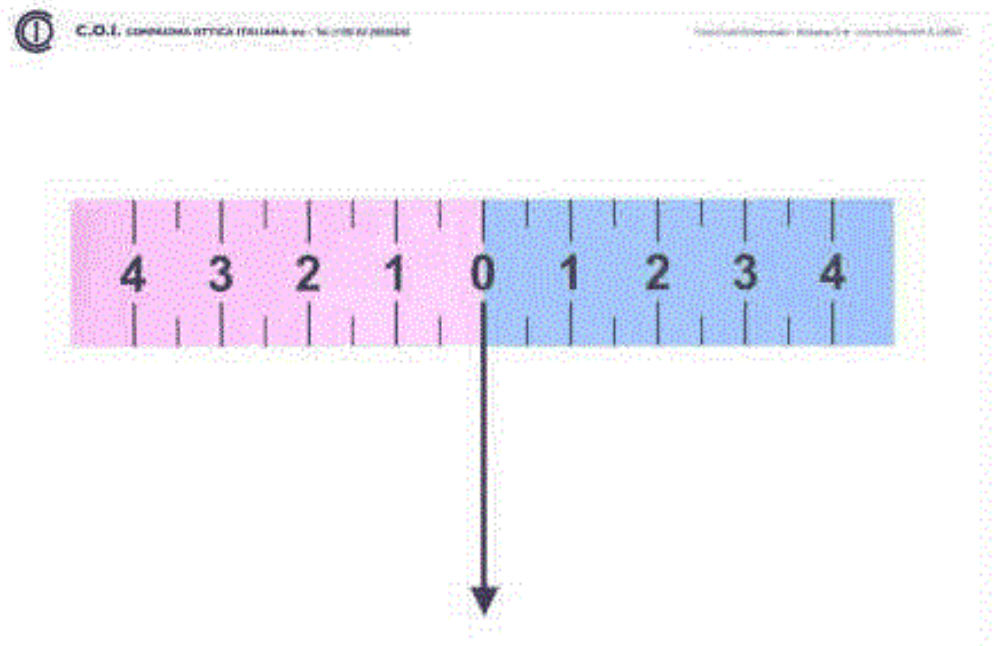
\includegraphics[scale=0.15]{source/immagini/foria_lontano.png}
  \captionof{figure}{Howell card lontano.}
  \label{fig:test1}
\end{minipage}%
\begin{minipage}{.5\textwidth}
  \centering
  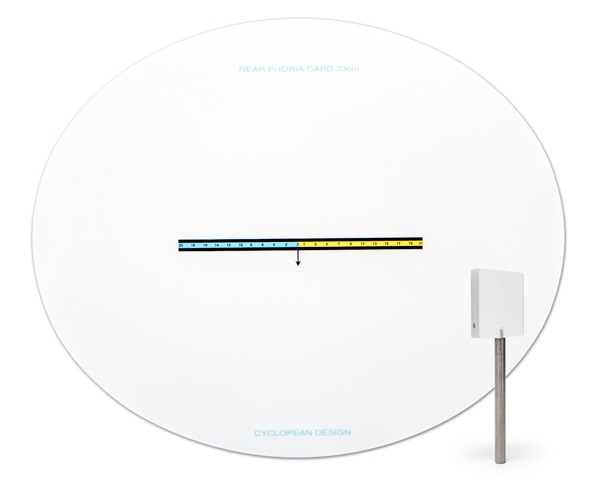
\includegraphics[scale=0.41]{source/immagini/foria_vicino.jpg}
  \captionof{figure}{Howell card vicino.}
  \label{fig:test2}
\end{minipage}
\end{figure}
\\\ \\\
\textbf{Punto prossimo di convergenza (PPC):} l’obiettivo era di valutare il punto di rottura e l’abilità del recupero della binocularità del soggetto. Si è voluto valutare come variava il PPC nella posizione in basso (45° sotto la posizione primaria), diritto e in alto (45° sopra la posizione primaria) per poter valutare se fosse presente lo stesso grado di binocularità in queste posizioni. É stato utilizzato come target una penlight e si chiedeva di osservare la luce finché non si fosse sdoppiata e riferire poi quanto tornava singola. È stata misurata in centimentri la distanza della pen light dagli occhi del soggetto. 
\\\ \\\
\textbf{Cover test:} il test è stato utilizzato per valutare e quantificare in modo oggettivo il funzionamento e la stabilità della muscolatura estrinseca dell’occhio. È stato effettuato mostrando la pen light ad una distanza di circa 40 cm nelle 9 posizioni di sguardo, seguendo l’H diagnostica come indicato in Figura 3.4, in modo da poter osservare le deviazioni degli occhi causate dall'azione dei muscoli oculari coinvolti. Infatti il cover test fornisce informazioni sulla stabilità binoculare del sistema visivo, quindi la capacità di recupero della binocularità del soggetto. Il test è stato ritenuto opportuno per indagare la funzione muscolare perchè è stato considerato che la stabilità binoculare sia data da due componenti: la percezione dello spazio che permette al cervello di localizzare la mira e l'azione dei muscoli oculari estrinseci che permettono lo spostamento dell'occhio nella direzione percepita corretta. Se quindi dovesse esserci un'imprecisione dell'azione muscolare, gli assi visivi potrebbero essere deviati producendo quindi una foria o tropia. La deviazione è stata quantificata con l’utilizzo dei prismi Base Interna per le exoforie/tropie, Base Esterna per le esoforie/tropie. 

Questo test inoltre è stato scelto per ottenere una misura fine della capacità muscolare del soggetto, altri test utilizzati solitamente per valutare l'abilità muscolare (DEM, NSUCO) non forniscono dati altrettanto precisi.
\\\
\begin{figure}[h!]
	\centering
	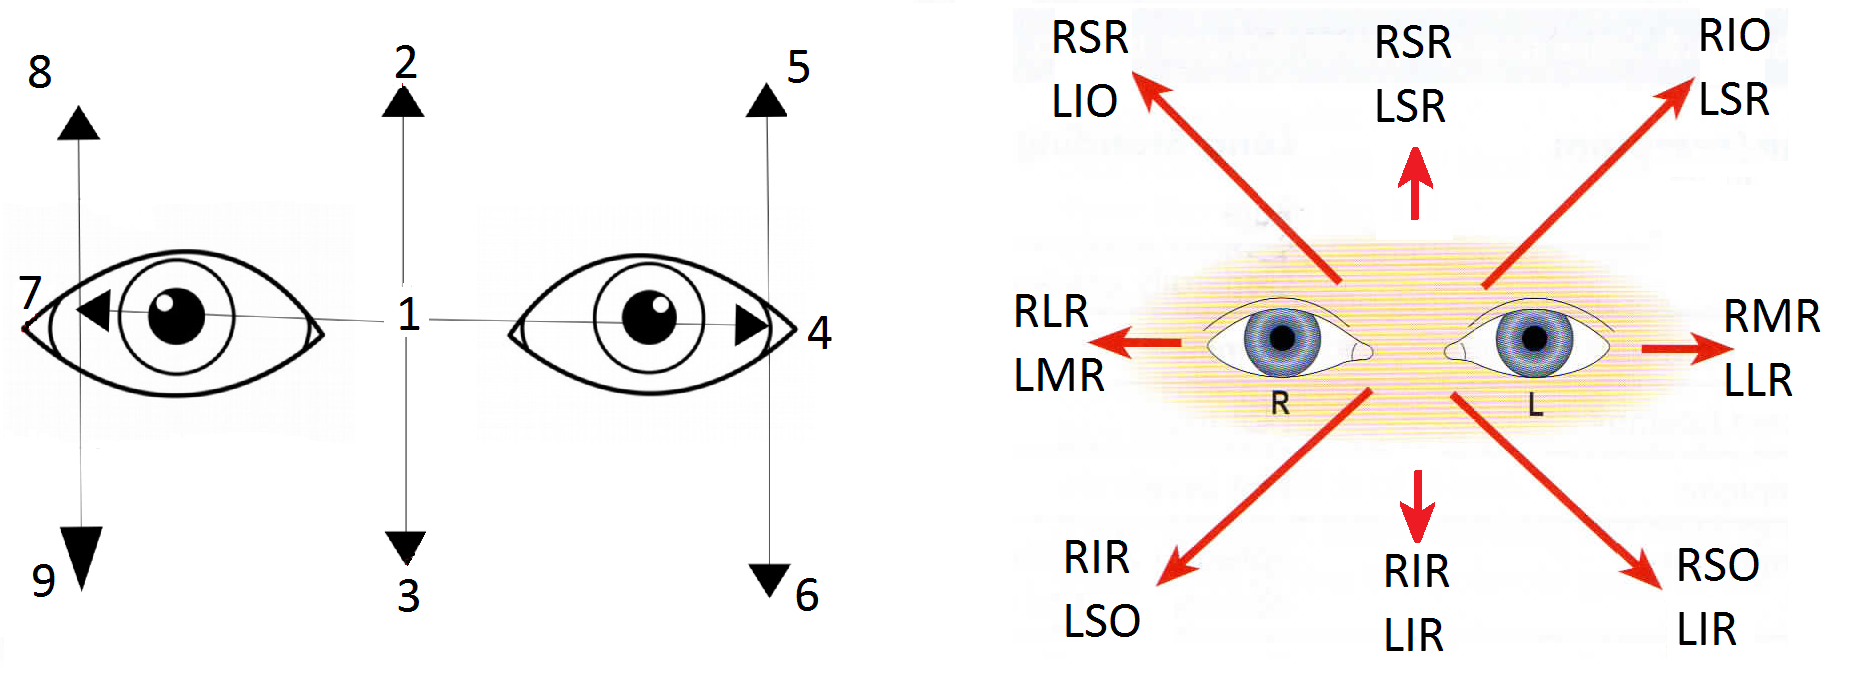
\includegraphics[scale=0.32]{source/immagini/immagine_cover_test(2).png}
	\caption[Wesson card]{Posizioni di sguardo indagate(sinistra) e muscoli stimolati(destra)}
	\label{fig:issuexample}
\end{figure}
\\\ \\\
\textbf{Ampiezza Accomodativa:} lo scopo era di valutare la capacità accomodativa del soggetto, valutata in rapporto con l’età. É stato utilizzato il metodo Push up per occhio destro, sinistro e binoculare, utilizzando come target i numeri della bacchetta di Lang (Figura 3.5) e quantificando in centimetri e non in diottrie per fare in modo di ottenere il miglioramento con una riduzione del valore, come accade negli altri test effettuati.

\begin{figure}[h!]
	\centering
	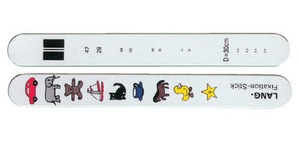
\includegraphics[scale=0.5]{source/immagini/ampiezza_accomodativa.jpg}
	\caption[Bacchetta di Lang per l'ampiezza accomodativa]{Bacchetta di Lang per l'ampiezza accomodativa.}
	\label{fig:issuexample}
\end{figure}
\\\ \\\ 
\textbf{Disparità di fissazione:} utilizzata per valutare la posizione degli assi visivi in condizioni binoculari. É stata mostrata
la Wesson Card utilizzando occhialini polarizzati e quantificandola in minuti d’arco.

\begin{figure}[h!]
	\centering
	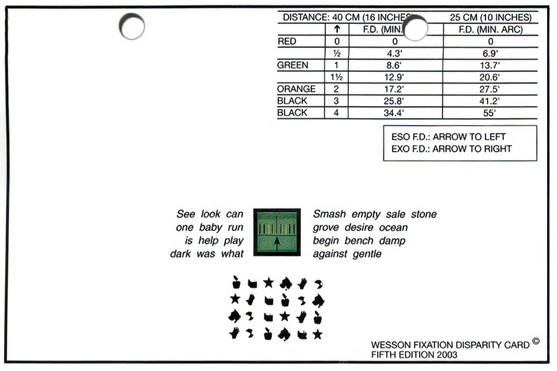
\includegraphics[scale=0.22]{source/immagini/Wesson_card.jpg}
	\caption[Wesson card]{Wesson card.}
	\label{fig:issuexample}
\end{figure}
\\\ \\\
\textbf{MEM:} il test è stato effettuato per valutare la posizione del piano accomodativo del soggetto, quantificato con lenti
positive per LAG e negative per LEAD.
\\\ \\\
\subsubsection{Valutazione e trattamento dello SMOF}

La valutazione del soggetto con squilibrio muscolare orofacciale comprende: 
\begin{enumerate}
\item \textbf{Raccolta anamnestica}
\begin{itemize}
 \item Anamnesi famigliare
 \item Anamnesi fisiologica sono state poste domande su: allattamento, presenza di abitudini viziate e parafunzioni, tipo di alimentazione, atteggiamenti posturali scorretti
  \item Anamnesi patologica si è indagata la presenza di patologie che possono aver facilitato l'esordio di una disfunzione muscolare orofacciale (traumi, carie, deviazioni del setto nasale o polipi nasali, allergie, frequenti infezioni delle vie respiratorie, otiti, perforazioni timpaniche)
\end{itemize}
\item \textbf{Esame obiettivo}, con lo scopo di valutare il tono e la funzione di distretti muscolari (orbicolare delle labbra, mentale, buccinatore, muscoli masticatori, muscoli del pavimento orale, muscoli linguali, nasali, diaframma, muscoli sopraioidei e sottoioidei)
\item \textbf{Analisi delle funzioni} dell'apparato stomatognatico (posizione linguale a riposo, durante l'atto deglutitorio ed in fonazione, masticazione, tipo e modalità di respirazione).
\end{enumerate}

Durante l’esame obiettivo si sono analizzate alcune caratteristiche del soggetto, quali la distanza naso-mento (se varia durante la deglutizione è un indice significativo di deglutizione deviata) e l'angolo cervico-pelvi-mandibolare (se ottuso, mostrato in Figura 3.7, potrebbe indicare deglutizione deviata).
\\\
Moyers distingue due tipi di deglutizione atipica: 
\begin{itemize}
 \itemsep-0.5em
  \item[--]Con  spinta  semplice:  contrazione  dei  muscoli  periorali,  contrazione  degli elevatori mandibolari, spinta linguale anteriore, arcate dentali a contatto
  \item[--]Con  spinta  complessa:  contrazione  dei  muscoli  periorali,  nessuna contrazione degli  elevatori  mandibolari,  spinta  linguale  anteriore  con lingua  e/o  labbro inferiore interposto tra le arcate dentali che non giungono, così, a contatto.
\end{itemize}
\\\ \\\
\begin{figure}[h!]
	\centering
	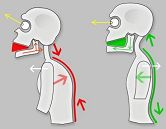
\includegraphics[scale=1.1]{source/immagini/angolo_cervico-pelvi-mandibolare.jpg}
	\caption[Differenza tra angolo cervico-pelvi-mandibolare ottuso e normale]{Differenza tra angolo cervico-pelvi-mandibolare ottuso (sinistra) e normale (destra).}
	\label{fig:issuexample}
\end{figure}
\\\ \\\
\textbf{Piano di trattamento}
\\\
In seguito è stato svolto il trattamento logopedico dello squilibrio muscolare orofacciale che si fonda soprattutto sui principi e sulla pratica della Terapia Miofunzionale. Quest’ultimo è un metodo rieducativo volto al raggiungimento di un equilibrio nel tono dei muscoli oro-facciali e alla correzione delle funzioni di pertinenza stomatognatica, quali la deglutizione, la fonazione, la masticazione e la respirazione. Il termine di “Myofunctional Therapy” (MFT) è stato coniato da Lischer nel 1918 e proposto all'American Society of Orthodontists da Rogers. Questi focalizzò l'attenzione sul ruolo determinante che ha il comportamento neuromuscolare nei confronti dello sviluppo dento-scheletrico e della terapia ortodontica. La stimolazione della muscolatura orofacciale può correggere in parte o completamente alcune dismorfosi dentali. Infatti i muscoli vengono considerati come “apparecchi ortodontici viventi" e vanno pertanto rieducati per stabilizzare e migliorare i risultati che si possono ottenere mediante il trattamento ortodontico.
\\\ \\\
Il piano terapeutico seguito dai soggetti dello studio è diviso in 3 fasi:
\begin{enumerate}
\item allenamento della muscolatura orofacciale con esercizi di rinforzo/rilassamento e stretching. In questa prima fase si utilizzano strumenti per rinforzare il tono dell’orbicolare delle labbra come nell’ “esercizio del bottone” (Figura 3.8), in cui il soggetto deve posizionare un bottone legato ad un filo tra denti e labbra e tirarlo, facendo resistenza con le labbra.

\begin{figure}[h!]
	\centering
	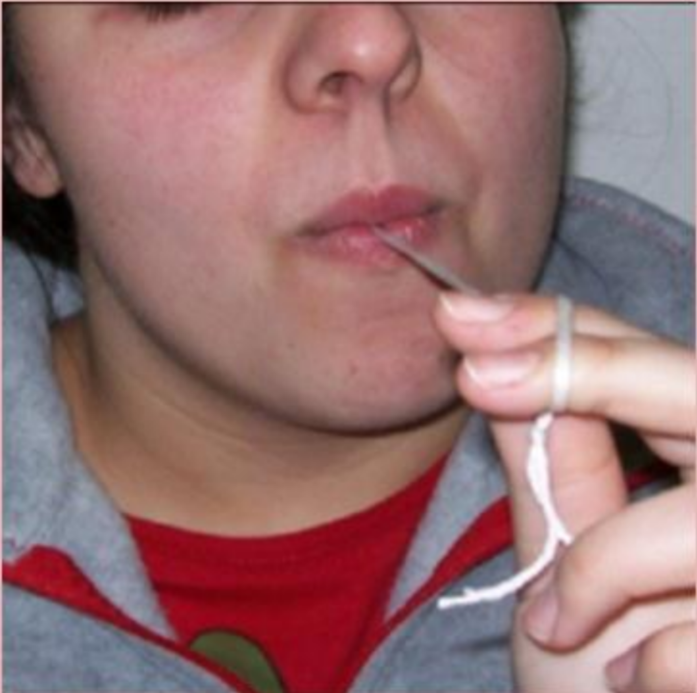
\includegraphics[scale=0.26]{source/immagini/esercizio_del_bottone.png}
	\caption[Esercizio del bottone]{Esercizio del bottone.}
	\label{fig:issuexample}
\end{figure}
 
Vengono proposti inoltre esercizi per allenare la postura linguale corretta, per esempio posizionando sull’apice della lingua un elastico ortodontico e chiedendo al soggetto di raggiungere e comprimere lo spot. Questo esercizio è utile anche per allenare l’atto deglutitorio corretto (Figura 3.9).

\begin{figure}[h!]
	\centering
	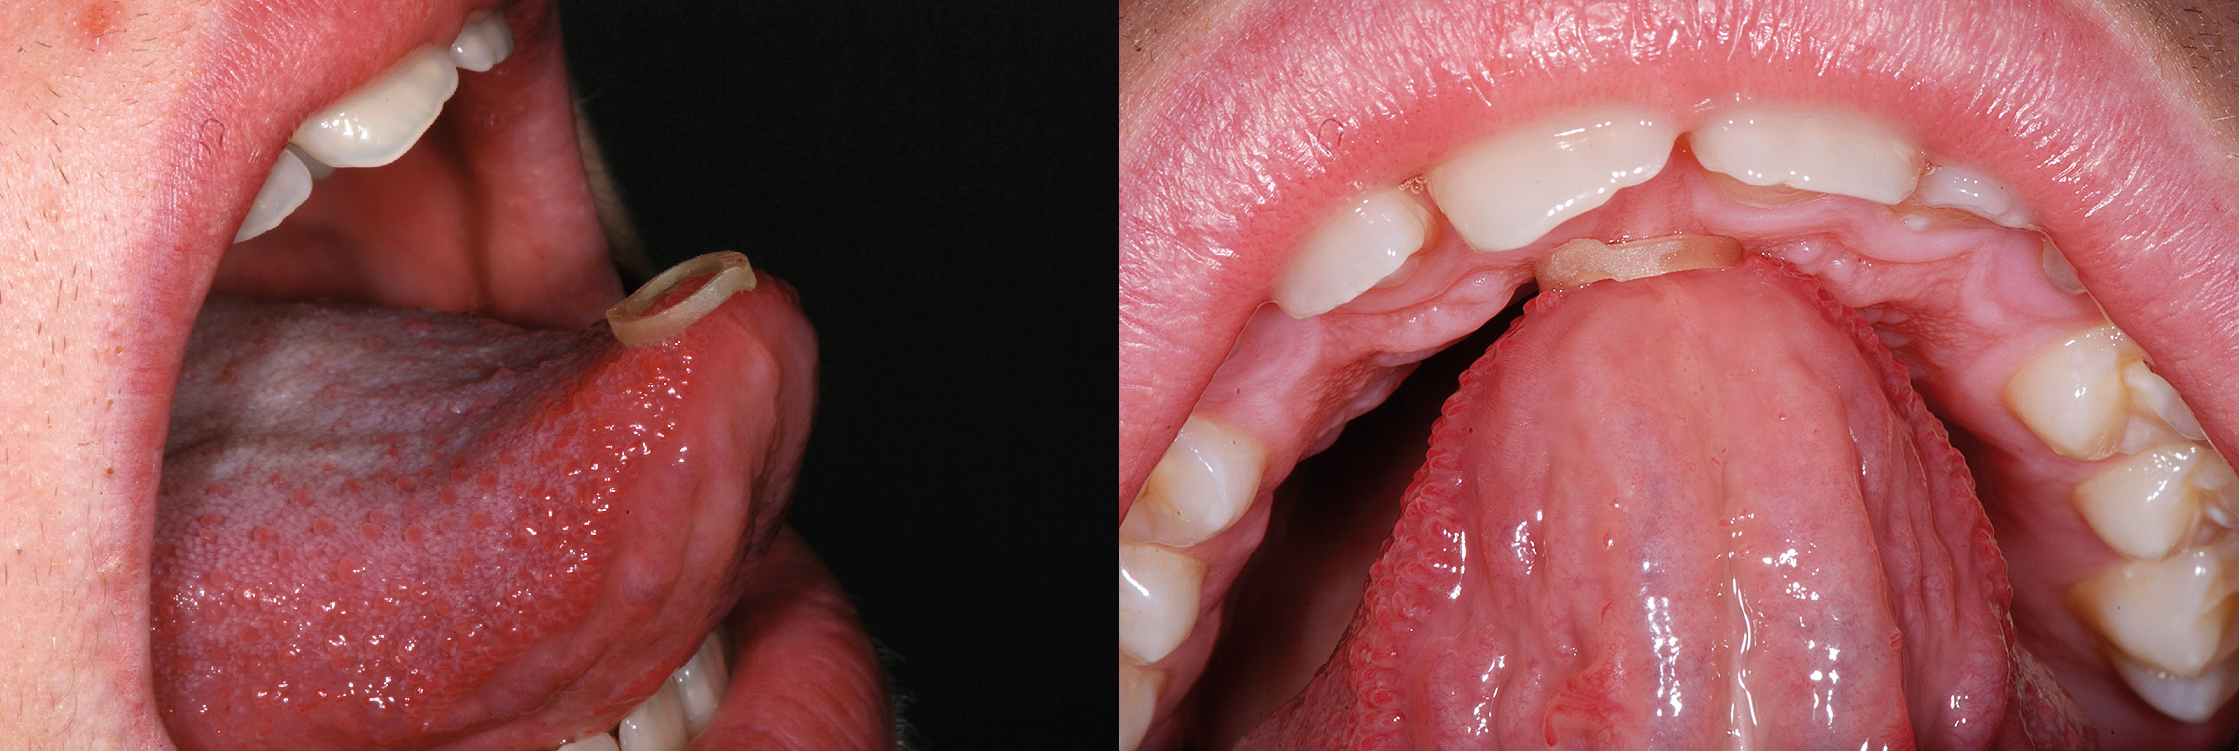
\includegraphics[scale=0.23]{source/immagini/esercizio_deglutizione.png}
	\caption[Posizionamento elastico e successiva compressione dello spot]{Posizionamento elastico(sinistra) e compressione dello spot(destra).}
	\label{fig:issuexample}
\end{figure}

Gli esercizi vanno eseguiti dal soggetto anche a domicilio almeno una volta al giorno, annotando su una griglia fornita dalla logopedista le sessioni di esercizi eseguite quotidianamente.
\item si insegna al soggetto a deglutire utilizzando cibi solidi e liquidi. Questa fase necessita di maggiore impegno da parte del soggetto, perché durante il pasto deve porre spesso attenzione a come posiziona la lingua mentre sta masticando e deglutendo.
\item si effettuano controlli periodici per verificare se gli esercizi vengono eseguiti correttamente e se l’atto deglutitorio e la postura linguale vengono automatizzati in modo corretto.
\end{enumerate}

Gli esercizi sono stati integrati con il trattamento osteopatico, il quale prevede un approccio globale ed uno locale. Il trattamento globale è stato indirizzato a correggere le disfunzioni più severe e strutturate valutate sul soggetto, interessanti l’apparato muscolo scheletrico e viscerale. Normalizzate queste, si passa ad un approccio mirato al distretto cefalico e alle strutture più intimamente correlate all’apparato stomatognatico dal punto di vista neurologico e tissutale. Si sono valutati e trattati specificamente le articolazioni della base e della volta cranica, il massiccio facciale, i muscoli masticatori, i muscoli sub-occipitali, muscoli sopra e sotto ioidei, il diaframma toracico.

\\\ \\\ \\\ \\\ 
\section{Analisi Statistica}

Per l’analisi statistica dei dati è stato utilizzato il software Libre Office Calc. È stata effettuata sia un’analisi descrittiva dei dati che un’analisi inferenziale di tutti i dati, per poi selezionare i più rappresentativi. 

La prima parte mostrerà l’analisi del campione descrivendolo per sesso e per età. Nella seconda parte sono riportati i dati in forma grafica, tramite istogrammi, confrontando le differenze presenti tra prima e dopo il trattamento sia nei soggetti trattati che nei non trattati. Per fare questo sono stati considerati i test che hanno riportato cambiamenti più evidenti dei valori medi. È stata effettuata anche l’analisi inferenziale tramite il test di Wilcoxon, per verificare se i cambiamenti osservati fossero anche statisticamente attendibili. Nell’ultima parte è stato descritto un caso clinico indicativo per mostrare il cambiamento avvenuto in seguito al
trattamento
\\\ \\\
\subsection{Analisi descrittive del campione}
I 19 soggetti rientrati nello studio sono stati divisi in 10 nel gruppo sperimentale e in 9 nel gruppo di controllo. Dei 10 soggetti del gruppo sperimentale 7 sono di sesso femminile e 3 di sesso maschile e il 50\% dei soggetti ha un’età inferiore o pari a 22 anni. Dei 9 soggetti del gruppo di controllo 4 sono di sesso femminile e 5 di sesso maschile e il 50\% dei soggetti ha un’età inferiore o pari a 22 anni. Nelle Tabelle 3.1 e 3.2 è riportata la sintesi delle caratteristiche dei soggetti che hanno partecipato alla ricerca.

\begin{table}[H]
\begin{center}
\begin{tabular}{|c|c|c|c|} \hline
{\textbf{}} & {\textbf{Maschio}} & {\textbf{Femmina}}& {\textbf{Totale}}\\ \hline
\textbf{Numero} & 8 & 11 & 19 \\ 
\textbf{Età} & 20.13 & 25.82 & \textbackslash \\ 
\textbf{Min.} & 10 & 12 & \textbackslash \\ 
\textbf{Max.} & 31 & 55 & \textbackslash \\ 
\textbf{Dev. Std.} & 6.13 & 13.04 & \textbackslash \\
\hline
\end{tabular}
\end{center}
\caption{Descrizione del campione diviso per sesso.}
\end{table}
\begin{table}[H]
\begin{center}
\begin{tabular}{|c|c|c|c|} \hline
{\textbf{}} & {\textbf{Trattati}} & {\textbf{Non trattati}}& {\textbf{Totale}}\\ \hline
\textbf{Maschio} & 3 & 5 & 8 \\
\textbf{Femmina} & 7 & 14 & 11\\ 
\textbf{Totale} & 10 & 9 & 19 \\ 
\textbf{Età} & 25.10 & 21.56 & \textbackslash \\ 
\textbf{Dev. Std.} & 14.52 & 4.42 & \textbackslash \\
\textbf{Mediana} & 22 & 22 & \textbackslash \\
\hline
\end{tabular}
\end{center}
\caption{Dati del campione diviso per gruppo di ricerca.}
\end{table}

Di seguito è stato riportato il calcolo e l’analisi dei valori medi del campione sperimentale.
La Tabella 3.3 riporta i valori di media, mediana e moda per tutti i test effettuati, confrontando i dati della prima valutazione ($\bar{x}_{prima}$, $\hat{x}_{prima}$, $\tilde{x}_{prima}$) con i dati della seconda valutazione ($\bar{x}_{dopo}$, $\hat{x}_{dopo}$, $\tilde{x}_{dopo}$) per i soggetti sottoposti al trattamento.

\begin{table}[H]
\begin{center}
\begin{tabular}{|c|c|c|c|c|c|c|} \hline
{\textbf{}} & {\textbf{$\bar{x}_{prima}$}}} & {\textbf{$\bar{x}_{dopo}$}}& {\textbf{$\hat{x}_{prima}$}}} & {\textbf{$\hat{x}_{dopo}$}}} & {\textbf{$\tilde{x}_{prima}$}}} & {\textbf{$\tilde{x}_{dopo}$}}}\\ \hline
\textbf{Sfero OD (D)} & -0.05 & -0.40 & 0.13 & 0.00 & 0.00 & 0.00 \\ \hline
\textbf{Cilindro OD (D)} & -0.45 & -0.35 & 0.00 & 0.00 & 0.00 & 0.00 \\ \hline
\textbf{Sfero OS (D)} & -0.20 & -0.35 & 0.13 & 0.00 & 0.00 & 0.00 \\ \hline
\textbf{Cilindro OS (D)} & -0.43 & -0.33 & 0.00 & 0.00 & 0.00 & 0.00 \\ \hline
\textbf{Foria L ($\Delta$)} & 0.00 & 0.05 & 0.00 & 0.25 & 0.00 & 0.50 \\ \hline
\textbf{Stereo L (sec d'arco)} & 184.00 & 190.00 & 30.00 & 30.00 & 30.00 & 30.00 \\ \hline
\textbf{PPC diritto (cm)} & \textbf{9.60} & \textbf{4.30} & \textbf{5.50} & \textbf{5.00} & \textbf{3.00} & \textbf{0.00} \\ \hline
\textbf{PPC alto (cm)} & 10.70 & 9.10 & 6.00 & 6.00 & 6.00 & 0.00\\ \hline
\textbf{PPC basso (cm)} & \textbf{7.80} & \textbf{1.10} & \textbf{0.50} & \textbf{0.00} & \textbf{0.00} & \textbf{0.00} \\ \hline
\textbf{Foria V alto ($\Delta$)} & 2.50 & 3.35 & 2.00 & 1.50 & 2.00 & 0.50 \\ \hline
\textbf{Foria V diritto ($\Delta$)} & 1.90 & 2.35 & 1.50 & 1.50 & 1.00 & 1.00 \\ \hline
\textbf{Foria V basso ($\Delta$)} & 2.65 & 2.10 & 2.00 & 1.50 & 2.00 & 1.00 \\ \hline
\textbf{CT 1 ($\Delta$)} & 7.40 & 6.60 & 7.00 & 6.50 & 2.00 & 6.00 \\ \hline
\textbf{CT 2 ($\Delta$)} & 10.30 & 11.80 & 12.00 & 11.00 & 0.00 & 8.00\\ \hline
\textbf{CT 3 ($\Delta$)} & 3.30 & 3.40 & 0.00 & 2.00 & 0.00 & 0.00 \\ \hline
\textbf{CT 4 ($\Delta$)} & 5.40 & 5.90 & 3.50 & 4.00 & 0.00 & 4.00 \\ \hline
\textbf{CT 5 ($\Delta$)} & 10.10 & 11.90 & 9.50 & 9.00 & 0.00 & 8.00 \\ \hline
\textbf{CT 6 ($\Delta$)} & 5.00 & 3.20 & 3.00 & 2.00 & 0.00 & 0.00 \\ \hline
\textbf{CT 7 ($\Delta$)} & \textbf{11.70} & \textbf{7.00} & \textbf{8.50} & \textbf{6.00} & \textbf{0.00} & \textbf{6.00} \\ \hline
\textbf{CT 8 ($\Delta$)} & \textbf{14.10} & \textbf{9.60} & \textbf{12.00} & \textbf{8.00} & \textbf{0.00} & \textbf{8.00} \\ \hline
\textbf{CT 9 ($\Delta$)} & 3.30 & 6.60 & 0.00 & 5.00 & 0.00 & 4.00 \\ \hline
\textbf{AA OD (cm)} & 8.70 & 10.20 & 8.00 & 9.00 & 4.00 & 6.00 \\ \hline
\textbf{AA OS (cm)} & 11.00 & 10.70 & 8.50 & 8.50 & 8.00 & 5.00 \\ \hline
\textbf{AA OO (cm)} & 8.00 & 8.90 & 7.00 & 7.00 & 8.00 & 5.00\\ \hline
\textbf{Stereo V (sec d'arco)} & \textbf{138.00} & \textbf{44.00} & \textbf{70.00} & \textbf{40.00} & \textbf{40.00} & \textbf{40.00}\\ \hline
\textbf{DF (min d'arco)} & 19.51 & 15.11 & 13.70 & 13.70 & 6.90 & 13.70 \\ \hline
\textbf{MEM OD (D)} & 0.85 & 0.88 & 1.00 & 1.00 & 1.00 & 1.25 \\ \hline
\textbf{MEM OS (D)} & 0.95 & 0.78 & 0.88 & 0.88 & 0.75 & 0.25 \\ \hline

\hline
\end{tabular}
\end{center}
\caption[Campione sperimentale: $\bar{x}$), ($\hat{x}$), ($\tilde{x}$, prima e dopo il trattamento]{Campione sperimentale: media($\bar{x}$), mediana($\hat{x}$) e moda($\tilde{x}$), prima e dopo il trattamento. Evidenziati i test con cambiamento maggiore.}
\end{table}

I dati che devono essere confrontati sono i valori della mediana, la quale ci informa che il 50\% dei soggetti ha presentato un dato non superiore al suo valore. Si vuole osservare un miglioramento dei valori dopo il trattamento. Per miglioramento si intende una riduzione del valore, quindi la differenza tra i dati pre e post trattamento deve essere maggiore di 0. Se si osservasse una variazione della mediana, si potrebbe supporre che almeno la metà del campione abbia riportato una riduzione del valore e quindi un miglioramento. 
\\\
I seguenti test riportano la presenza di un cambiamento positivo nella mediana almeno di 0,50 unità:

\begin{itemize}
 \itemsep-0.5em
 \item[--]Punto prossimo di convergenza diritto e basso
 \item[--]Foria vicino alto e basso
 \item[--]Cover test in posizione 1 (diritto)
 \item[--]Cover test in posizione  2 (alto in centro; stimolazione: retti superiori entrambi gli occhi)
 \item[--]Cover test in posizione 5 (in alto a sinistra; stimolazione: retto superiore OS, obliquo inferiore OD)
 \item[--]Cover test in posizione  6 (in basso a sinistra; muscoli stimolati: obliquo superiore destro e retto inferiore sinistro)
 \item[--]Cover test in posizione 7 (a destra; muscoli stimolati: retto esterno destro, retto mediale sinistro)
 \item[--]Cover test in posizione 8 (in alto a destra; muscoli stimolati: retto superiore destro, obliquo inferiore sinistro).
 \item[--]Stereopsi vicino
\end{itemize}
\\\
I test che hanno riportato un minimo cambiamento positivo (0,25 unità) o nullo sono:
\begin{itemize}
 \itemsep-0.5em
 \item[--]cilindro e sfero
 \item[--]Foria lontano
 \item[--]Stereopsi lontano
 \item[--]PPC alto
 \item[--]Foria vicino diritto
 \item[--]Ampiezza accomodativa OS
 \item[--]MEM
 \end{itemize}
\\\
I test che hanno riportato un peggioramento sono:
\begin{itemize}
 \itemsep-0.5em
 \item[--]Cover test in posizione 3 (in basso al centro; stimolazione: retti inferiori entrambi gli occhi)
 \item[--]Cover test in posizione 4 (a sinistra; stimolazione: retto laterale OS, retto mediale OD)
 \item[--]Cover test in posizione 9 (in basso a destra; stimolazione: obliquo superiore OS, retto inferiore OD)
 \item[--]Ampiezza accomodativa OD e binoculare
 \item[--]Disparità di fissazione
 \end{itemize}
 
 
 
\subsection{Analisi e discussione dei dati}
 
In questa sezione verrà verificato se è possibile riscontrare un cambiamento statisticamente significativo tra gli esiti dei test effettuati prima e dopo il trattamento logopedico-osteopatico.
 
Il confronto statistico tra i dati della prima e della seconda valutazione è stato misurato utilizzando il test di Wilcoxon (Wilcoxon paired-sample test), il quale si applica nel confronto di dati appaiati quando la variabile in esame non è distribuita in maniera normale. Esso è l’equivalente per dati appaiati del test di Student e può essere effettuato anche per piccoli campioni. L’ipotesi nulla afferma che non ci sia stato alcun cambiamento tra prima e dopo il trattamento. Il livello di significatività è stato posto a 0.05 e il test è a due code. Si considerano i valori della prima valutazione appaiati con quelli della seconda valutazione. In appendice sono riportati i dati ottenuti dalle analisi visive, calcolando la differenza tra pre e post trattamento. Se la differenza è positiva allora è stato riscontrato un miglioramento, se è pari a 0 allora la condizione è rimasta invariata, se è negativa significa peggioramento. Questo test è stato applicato a tutti i dati ottenuti dalle valutazioni, ma in particolare verranno analizzati solo i test: PPC diritto, PPC basso, CT in posizione 7, CT in posizione 8 e Stereopsi vicino. Questi sono infatti i test che hanno riportato un maggiore miglioramento dei valori medi, quindi si va ad osservare se esso può anche essere considerato statisticamente significativo. 
\\\ \\\
\subsubsection{Punto prossimo di convergenza (PPC) diritto}

Nella Tabella 3.4 e 3.5 sono mostrati i valori medi dei dati del punto di rottura del PPC in posizione diritta rispettivamente per il gruppo dei trattati e per il gruppo dei non trattati. Nella Tabella 3.6 e 3.7 sono invece riportati i valori medi dei dati del punto di recupero per, rispettivamente, gruppo dei trattati e gruppo dei non trattati.

Osservando le tabelle dei dati in appendice, in seguito al trattamento, si nota che nel gruppo sperimentale 5 (50\%) soggetti hanno punti di rottura più vicini, uno (10\%) rimane invariato, mentre 4 (40\%) hanno punti di rottura più distali. Il recupero invece per 8 (80\%) soggetti si trova ad una distanza minore, mentre per 2 (20\%) soggetti a distanza maggiore. 
\\\ \\\
A distanza di 3 mesi dalla prima visita nel gruppo di controllo si hanno 2 (22,2\%) soggetti che riportano punti di rottura più ravvicinati, 2 (22,2\%) rimangono invariati e 5 (55,5\%) riportano valori più distali. Il punto di recupero per 3 (33,3\%) soggetti del gruppo di controllo è più vicino, 1 (11,1\%) è rimasto invariato mentre per 5 (55,5\%) soggetti è più lontano. 

Negli istogrammi (Figura 3.10, 3.11, 3.12 e 3.13), sull’asse delle ascisse sono riportati i valori centrali degli intervalli che rappresentano i dati raccolti del punto di rottura/recupero, mentre sull’asse delle ordinate sono presenti le frequenze riscontrate per ogni intervallo. Sono riportati sia il grafico del gruppo sperimentale che quello del gruppo di controllo e le colonne blu si riferiscono ai dati della prima valutazione, mentre quelle rosse ai dati della seconda valutazione.
%%%%%%%%%%%%%%%%%%
\begin{table}
\centering
\setlength\tabcolsep{4pt}
\begin{minipage}{0.48\textwidth}
\centering
\tablewidth=\textwidth

\begin{tabular}{|c|c|c|} \hline
{\textbf{}} & {\textbf{  \hspace{8pt}Prima\hspace{8pt} }} & {\textbf{ \hspace{8pt}Dopo\hspace{8pt}  }}\\ \hline
\textbf{Numeri dati} & 10 & 10 \\ 
\textbf{Media} & 9.60 & 4.30 \\  
\textbf{Dev. Std.} & 11.81 & 3.40 \\  
\textbf{Mediana} & 5.50 & 5.00 \\ 
\textbf{Moda} & 3.00 & 0.00 \\ 
\textbf{Errore Std.} & 12.49 & 3.61 \\ 
\hline
\end{tabular}
\caption{Dati gruppo sperimentale PPC rottura diritto.}

\label{tab:accuracy} 
\end{minipage}%
\hfill
\begin{minipage}{0.48\textwidth}
\centering

\begin{tabular}{|c|c|c|} \hline
{\textbf{}} & {\textbf{  \hspace{8pt}Prima\hspace{8pt} }} & {\textbf{ \hspace{8pt}Dopo\hspace{8pt}  }}\\ \hline
\textbf{Numeri dati} & 9 & 9 \\ 
\textbf{Media} & 9.89 & 7.44 \\  
\textbf{Dev. Std.} & 14.28 & 6.54 \\  
\textbf{Mediana} & 6.00 & 5.00 \\  
\textbf{Moda} & 0.00 & \textbackslash \\
\textbf{Errore Std.} & 14.51 & 6.33 \\
\hline
\end{tabular}
\caption{Dati gruppo di controllo PPC rottura diritto.}

 \label{tab:ompdiff} 
\end{minipage}
\hfill
\begin{minipage}{0.48\textwidth}
\centering

\begin{tabular}{|c|c|c|} \hline
{\textbf{}} & {\textbf{  \hspace{8pt}Prima\hspace{8pt} }} & {\textbf{ \hspace{8pt}Dopo\hspace{8pt}  }}\\ \hline
\textbf{Numeri dati} & 10 & 10 \\
\textbf{Media} & 14.20 & 7.40 \\  
\textbf{Dev. Std.} & 12.32 & 7.72 \\ 
\textbf{Mediana} & 9.00 & 7.00 \\ 
\textbf{Moda} & 8.00 & 0.00 \\ 
\textbf{Errore Std.}& 12.82 & 8.17 \\ 
\hline
\end{tabular}
\caption{Dati gruppo sperimentale PPC recupero diritto.}

\label{tab:accuracy} 
\end{minipage}%
\hfill
\begin{minipage}{0.48\textwidth}
\centering

\begin{tabular}{|c|c|c|} \hline
{\textbf{}} & {\textbf{  \hspace{8pt}Prima\hspace{8pt} }} & {\textbf{ \hspace{8pt}Dopo\hspace{8pt}  }}\\ \hline
\textbf{Numeri dati} & 9 & 9 \\ 
\textbf{Media} & 13.56 & 10.33 \\  
\textbf{Dev. Std.} & 16.36 & 7.75 \\  
\textbf{Mediana} & 9.00 & 8.00 \\ 
\textbf{Moda} & 0.00 & 8.00 \\ 
\textbf{Errore Std.} & 16.45 & 7.30\\ 
\hline
\end{tabular}
\caption{Dati gruppo di controllo PPC recupero diritto.}

 \label{tab:ompdiff} 
\end{minipage}
\end{table}
%%%%%%%%%%%%%%%%%%%%%

Il test di Wilcoxon riporta per il punto di rottura un W-value di 14.5 il quale, essendo superiore al valore critico (critical value=5), riferisce che il cambiamento non può essere considerato statisticamente significativo. Per il punto di recupero viene riportato un W-value pari a 10.5, con valore critico a 8. Quindi anche per il punto di recupero il cambiamento è non significativo. Osservando però gli istogrammi riportati è possibile notare uno spostamento dei dati verso valori inferiori, quindi con lo spostamento delle colonne rosse verso sinistra. Inoltre dai dati presenti in appendice è possibile notare che un cambiamento è stato effettivamente rilevato, anche se non è stato valutato come statisticamente significativo dal test di Wilcoxon. Infatti il 50\% dei soggetti trattati migliora il valore del punto di rottura e l’80\% riduce il valore del punto di recupero. Al contrario nel gruppo di controllo si riscontra un miglioramento del punto di rottura solo per il 22,2\%, e per il 33,3\% un miglioramento del punto di recupero.

 \begin{figure}[h!]
	\centering
	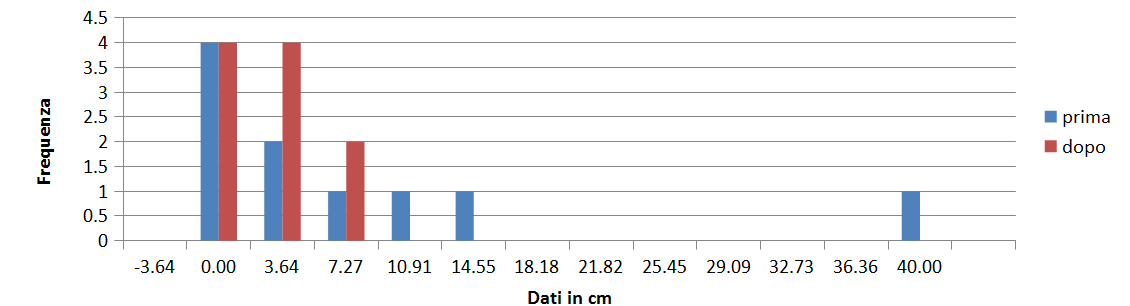
\includegraphics[scale=0.37]{source/grafici/PPC_DIRITTO_DEFINITIVO_sperimentale.png}
	\caption[Istogramma gruppo sperimentale per punto di rottura PPC (diritto)]{Istogramma gruppo sperimentale per punto di rottura PPC (diritto): confronto tra prima e seconda valutazione.}
	\label{fig:issuexample}
\end{figure}
 \begin{figure}[h!]
	\centering
	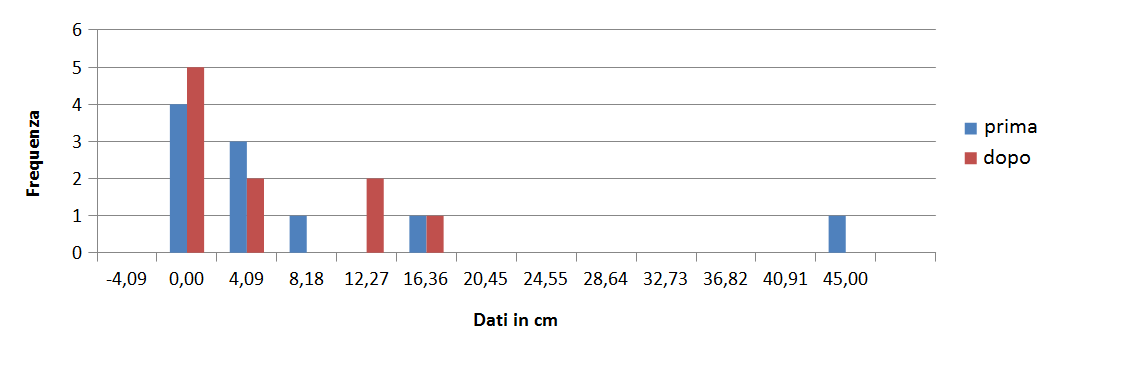
\includegraphics[scale=0.37]{source/grafici/PPC_DIRITTO_DEFINITIVO_GRUPPO_CONTROLLO.png}
	\caption[Istogramma gruppo di controllo per punto di rottura PPC (diritto)]{Istogramma gruppo di controllo per punto di rottura PPC (diritto): confronto tra prima e seconda valutazione.}
	\label{fig:issuexample}
\end{figure}
 \begin{figure}[h!]
	\centering
	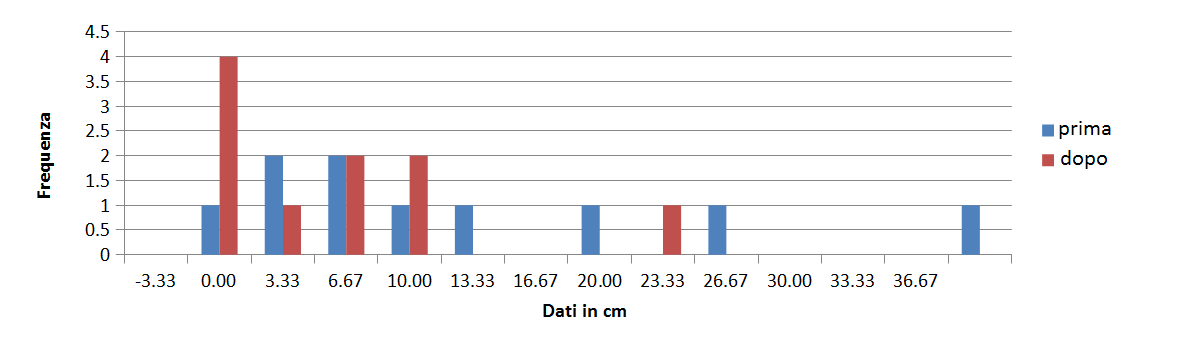
\includegraphics[scale=0.37]{source/grafici/Recupero_PPC_diritto_Trattati.png}
	\caption[Istogramma  sperimentale per punto di recupero PPC (diritto)]{Istogramma  sperimentale per punto di recupero PPC (diritto): confronto tra prima e seconda valutazione.}
	\label{fig:issuexample}
\end{figure}
 \begin{figure}[h!]
	\centering
	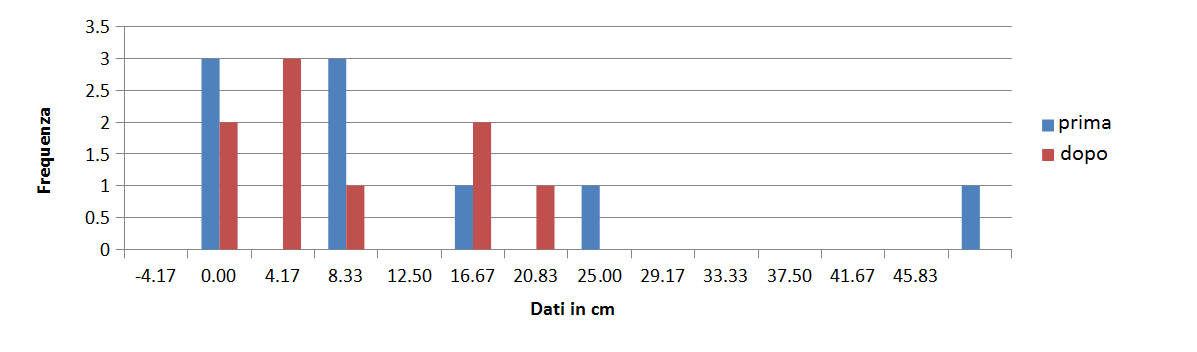
\includegraphics[scale=0.37]{source/grafici/Recupero_PPC_diritto_Non_Trattati.png}
	\caption[Istogramma gruppo di controllo per punto di recupero PPC (diritto)]{Istogramma gruppo di controllo per punto di recupero PPC (diritto): confronto tra prima e seconda valutazione.}
	\label{fig:issuexample}
\end{figure}
\\\ \\\
\subsubsection{Punto prossimo di convergenza (PPC) basso}

Il punto prossimo di convergenza è stato valutato anche con lo sguardo rivolto a 45° sotto la posizione primaria. Questo è utile per comprendere se il soggetto possiede una migliore binocularità durante le attività svolte da vicino. Nelle tabelle 3.8 , 3.9, 3.10 e 3.11 sono riportati i valori medi dei punti di rottura e recupero del gruppo dei trattati e non trattati. In appendice invece sono riportati tutti i dati rilevati durante le valutazioni, a cui si fa riferimento per le successive considerazioni.

Nel gruppo dei trattati  4 soggetti (40\%) rompono a distanze minori, 4 soggetti (40\%) rimangono invariati e 2 (20\%) rompono a maggiore distanza; invece 4 soggetti (40\%) recuperano prima, 4 (40\%) rimangono invariati e 2 (2\%) recuperano più lontano. 
Nel gruppo di controllo si hanno 3 soggetti (33,3\%) che rompono prima, 2 (22,2\%) rimangono invariati e 4 (44,4\%) peggiorano; mentre 4 soggetti (44,4\%) recuperano prima, 3 (33,3\%) rimangono invariati e 2 (22,2\%) recuperano più lontano.
%%%%%%%%%%%%%%%%%%
\begin{table}
\centering
\setlength\tabcolsep{4pt}
\begin{minipage}{0.48\textwidth}
\centering
\tablewidth=\textwidth

\begin{tabular}{|c|c|c|} \hline
{\textbf{}} & {\textbf{  \hspace{8pt}Prima\hspace{8pt} }} & {\textbf{ \hspace{8pt}Dopo\hspace{8pt}  }}\\ \hline
\textbf{Numeri dati} & 10 & 10 \\ 
\textbf{Media} & 7.8 & 1.10 \\  
\textbf{Dev. Std.} & 13.05 & 1.79 \\  
\textbf{Mediana} & 0.50 & 0.00 \\ 
\textbf{Moda} & 0.00 & 0.00 \\ 
\textbf{Errore Std.} & 13.80 & 1.57 \\ 
\hline
\end{tabular}
\caption{Dati gruppo sperimentale PPC rottura basso.}

\label{tab:accuracy} 
\end{minipage}%
\hfill
\begin{minipage}{0.48\textwidth}
\centering

\begin{tabular}{|c|c|c|} \hline
{\textbf{}} & {\textbf{  \hspace{8pt}Prima\hspace{8pt} }} & {\textbf{ \hspace{8pt}Dopo\hspace{8pt}  }}\\ \hline
\textbf{Numeri dati} & 9 & 9 \\ 
\textbf{Media} & 7.89 & 6.56 \\  
\textbf{Dev. Std.} & 14.54 & 6.44 \\  
\textbf{Mediana} & 4.00 & 6.00 \\  
\textbf{Moda} & 0.00 & 6.00 \\
\textbf{Errore Std.} & 15.49 & 6.28 \\
\hline
\end{tabular}
\caption{Dati gruppo di controllo PPC rottura basso.}

 \label{tab:ompdiff} 
\end{minipage}
\hfill
\begin{minipage}{0.48\textwidth}
\centering

\begin{tabular}{|c|c|c|} \hline
{\textbf{}} & {\textbf{  \hspace{8pt}Prima\hspace{8pt} }} & {\textbf{ \hspace{8pt}Dopo\hspace{8pt}  }}\\ \hline
\textbf{Numeri dati} & 10 & 10 \\
\textbf{Media} & 10.70 & 2.70 \\  
\textbf{Dev. Std.} & 15.24 & 4.52 \\ 
\textbf{Mediana} & 2.00 & 0.00 \\ 
\textbf{Moda} & 0.00 & 0.00 \\ 
\textbf{Errore Std.}& 15.73 & 4.20 \\ 
\hline
\end{tabular}
\caption{Dati gruppo sperimentale PPC recupero basso.}

\label{tab:accuracy} 
\end{minipage}%
\hfill
\begin{minipage}{0.48\textwidth}
\centering

\begin{tabular}{|c|c|c|} \hline
{\textbf{}} & {\textbf{  \hspace{8pt}Prima\hspace{8pt} }} & {\textbf{ \hspace{8pt}Dopo\hspace{8pt}  }}\\ \hline
\textbf{Numeri dati} & 9 & 9 \\ 
\textbf{Media} & 10.67 & 10.00 \\  
\textbf{Dev. Std.} & 16.06 & 7.97 \\  
\textbf{Mediana} & 8.00 & 9.00 \\ 
\textbf{Moda} & 0.00 & 0.00 \\ 
\textbf{Errore Std.} & 17.11 & 7.55\\ 
\hline
\end{tabular}
\caption{Dati gruppo di controllo PPC recupero basso.}

 \label{tab:ompdiff} 
\end{minipage}
\end{table}
%%%%%%%%%%%%%%%%%%%%%

Negli istogrammi riportati nelle figure 3.14, 3.15, 3.16 e 3.17 si rappresenta sull’asse delle ascisse i valori medi dei dati raccolti misurati in centimetri, mentre sull’asse delle ordinate le frequenze con cui questi valori medi si presentano all’interno del campione. Le colonne blu si riferiscono alla prima valutazione mentre le colonne rosse alla seconda.
\\\ \\\ \\\ \\\
Analizzando i dati utilizzando il test di Wilcoxon si ottiene per il punto di rottura un W-value pari a 3, con valore critico posto a 0, mentre per il punto di recupero si ottiene un W-value pari a 4 con valore critico a 0. Questi cambiamenti non sono quindi da considerarsi statisticamente significativi. Negli istogrammi viene evidenziato uno spostamento delle colonne rosse verso sinistra soprattutto per il punto di rottura. Nonostante ciò, nelle percentuali non è possibile osservare un cambiamento evidente, infatti i valori sono uniformi per entrambi i gruppi. 

Nei test del punto prossimo di convergenza il cambiamento non è risultato statisticamente significativo per un motivo di ampiezza del campione, però anche la presenza di variabili che non sono state considerate in sede di organizzazione della ricerca potrebbero aver influito sulla valutazione. La variabile più influente sul punto prossimo di convergenza è la stanchezza. È infatti possibile che le condizioni in cui sono state sottoposte le valutazioni non siano le stesse per il gruppo dei trattati e per il gruppo di controllo e quindi questo potrebbe aver influito negativamente sui risultati.
 \begin{figure}[h!]
	\centering
	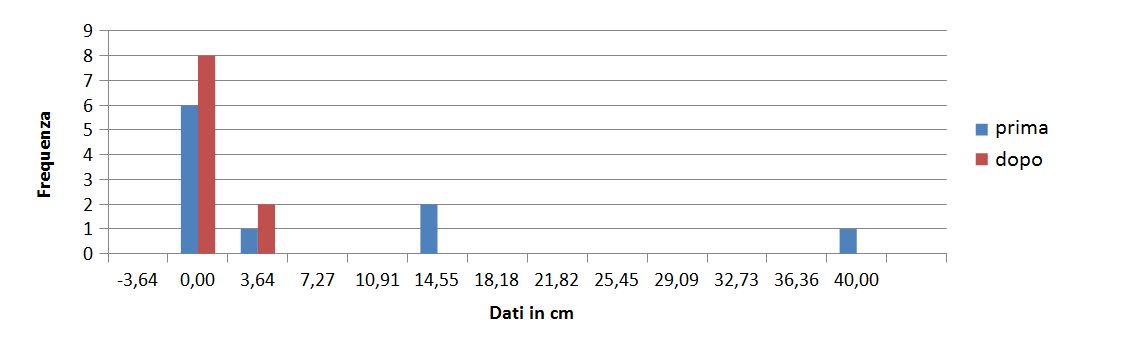
\includegraphics[scale=0.38]{source/grafici/PPC_BASSO_DEFINITIVO.png}
	\caption[Istogramma gruppo sperimentale per punto di rottura PPC (basso)]{Istogramma gruppo sperimentale per punto di rottura PPC (basso): confronto tra prima e seconda valutazione.}
	\label{fig:issuexample}
\end{figure}
 \begin{figure}[h!]
	\centering
	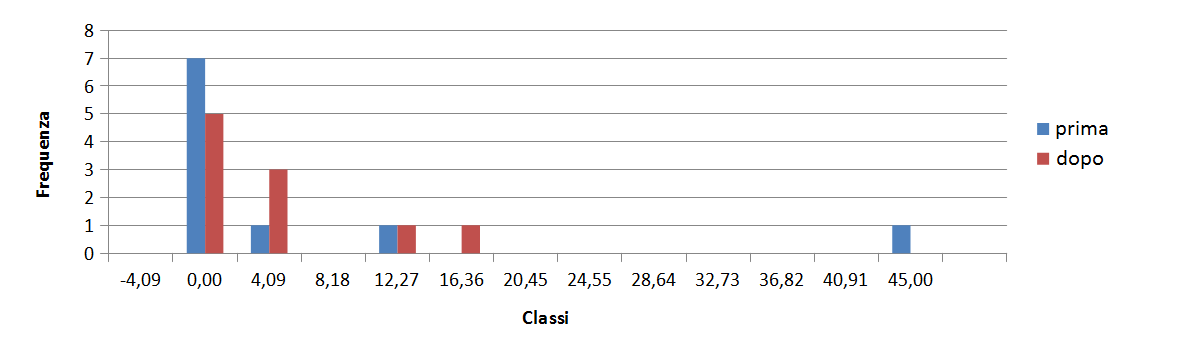
\includegraphics[scale=0.38]{source/grafici/PPC_BASSO_CONTROLLO.png}
	\caption[Istogramma gruppo di controllo per punto di rottura PPC (basso)]{Istogramma gruppo di controllo per punto di rottura PPC (basso): confronto tra prima e seconda valutazione.}
	\label{fig:issuexample}
\end{figure}
 \begin{figure}[h!]
	\centering
	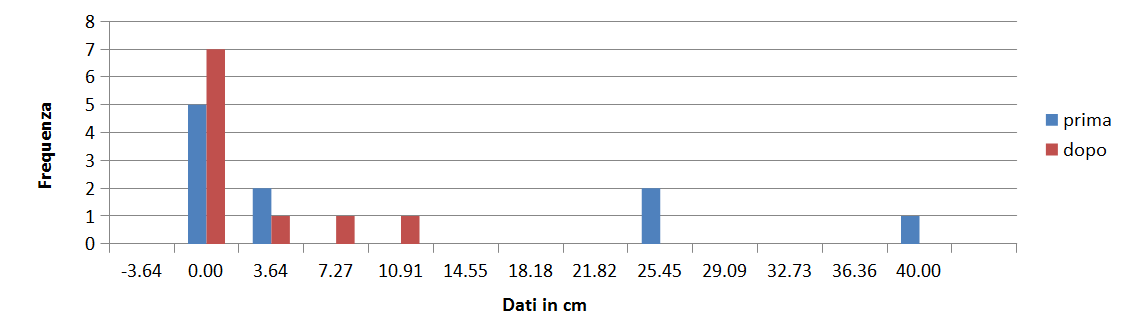
\includegraphics[scale=0.38]{source/grafici/Grafico_recupero_PPC_basso_trattati.png}
	\caption[Istogramma gruppo sperimentale per punto di recupero PPC (basso)]{Istogramma gruppo sperimentale per punto di recupero PPC (basso): confronto tra prima e seconda valutazione.}
	\label{fig:issuexample}
\end{figure}
 \begin{figure}[h!]
	\centering
	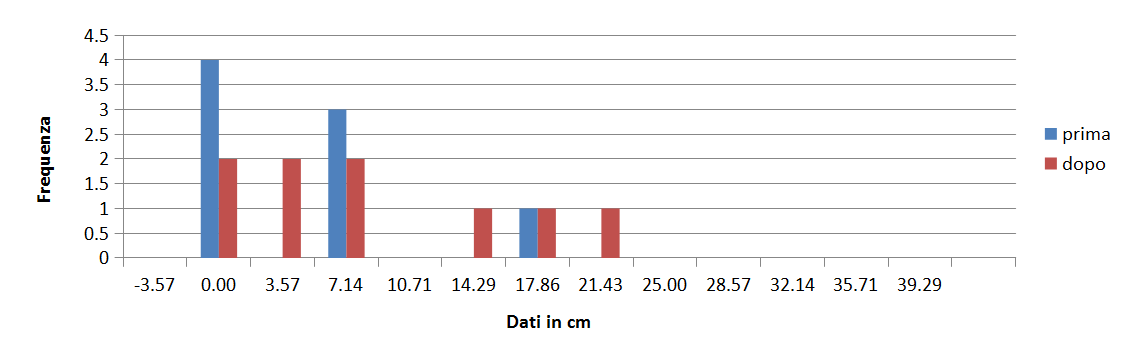
\includegraphics[scale=0.38]{source/grafici/Grafico_recupero_PPC_basso_NON_trattati.png}
	\caption[Istogramma gruppo di controllo per punto di recupero PPC (basso)]{Istogramma gruppo di controllo per punto di recupero PPC (basso): confronto tra prima e seconda valutazione.}
	\label{fig:issuexample}
\end{figure}
\\\ \\\  \\\ \\\ \\\ \\\
\subsubsection{Cover test in posizione 7}

La posizione 7 corrisponde allo sguardo rivolto a destra, stimolando i muscoli retto esterno dell’occhio destro e il retto interno dell’occhio sinistro. I dati sono stati presi con il valore assoluto, senza considerare se si trattava di eso/exo foria o eso/exo tropia, dal momento che non cambiava l’entità del difetto, ma la sua quantità. In appendice sono riportati i valori e il segno (s) corrisponde a esoforia/tropia, mentre (x) a exoforia/tropia. 

Nel gruppo sperimentale 6 (60\%) soggetti riportano un miglioramento, uno (10\%) rimane invariato e 3 (30\%) sono peggiorati. Nel gruppo di controllo 3 (33,3\%) soggetti riportano un miglioramento, 3 (33,3\%) sono invariati e 3 (33,3\%) sono peggiorati. Nella Tabella 3.12 e 3.13 vengono inseriti i valori medi del gruppo sperimentale e del gruppo di controllo. Nelle Figure 3.18 e 3.19 sono riportati gli istogrammi che rappresentano i dati ottenuti nella prima valutazione (colonne blu) e seconda valutazione (colonne rosse).

Il test di Wilcoxon fornisce un W-value di 17 con valore critico a 5. Il cambiamento non è quindi da considerarsi statisticamente significativo. Anche in questi istogrammi però è possibile notare lo spostamento delle colonne rosse verso sinistra, indicando che effettivamente un buon numero di soggetti (60\%) ha riscontrato un miglioramento dei valori, verificabile anche osservando i dati riportati in appendice. Stessa cosa non può essere detta per i soggetti appartenenti al gruppo di controllo, dove solo il 33,3\% ha riportato un miglioramento dei dati.

%%%%%%%%%%%%%%%%%%
\begin{table}
\centering
\setlength\tabcolsep{4pt}
\begin{minipage}{0.48\textwidth}
\centering
\tablewidth=\textwidth

\begin{tabular}{|c|c|c|} \hline
{\textbf{}} & {\textbf{  \hspace{8pt}Prima\hspace{8pt} }} & {\textbf{ \hspace{8pt}Dopo\hspace{8pt}  }}\\ \hline
\textbf{Numeri dati} & 10 & 10 \\ 
\textbf{Media} & 11.70 & 7.00 \\  
\textbf{Dev. Std.} & 14.04 & 4.64 \\  
\textbf{Mediana} & 8.50 & 6.00 \\ 
\textbf{Moda} & 0.00 & 6.00 \\ 
\textbf{Errore Std.} & 14.89 & 4.81 \\ 
\hline
\end{tabular}
\caption{Dati gruppo sperimentale Cover test 7.}

\label{tab:accuracy} 
\end{minipage}%
\hfill
\begin{minipage}{0.48\textwidth}
\centering

\begin{tabular}{|c|c|c|} \hline
{\textbf{}} & {\textbf{  \hspace{8pt}Prima\hspace{8pt} }} & {\textbf{ \hspace{8pt}Dopo\hspace{8pt}  }}\\ \hline
\textbf{Numeri dati} & 9 & 9 \\ 
\textbf{Media} & 10.78 & 10.00 \\  
\textbf{Dev. Std.} & 4.41 & 3.46 \\  
\textbf{Mediana} & 12.00 & 8.00 \\  
\textbf{Moda} & 12.00 & 8.00 \\
\textbf{Errore Std.} & 3.84 & 3.70 \\
\hline
\end{tabular}
\caption{Dati gruppo di controllo Cover test 7.}

 \label{tab:ompdiff} 
\end{minipage}
\end{table}
%%%%%%%%%%%%%%%%%%%%%
 \begin{figure}[h!]
	\centering
	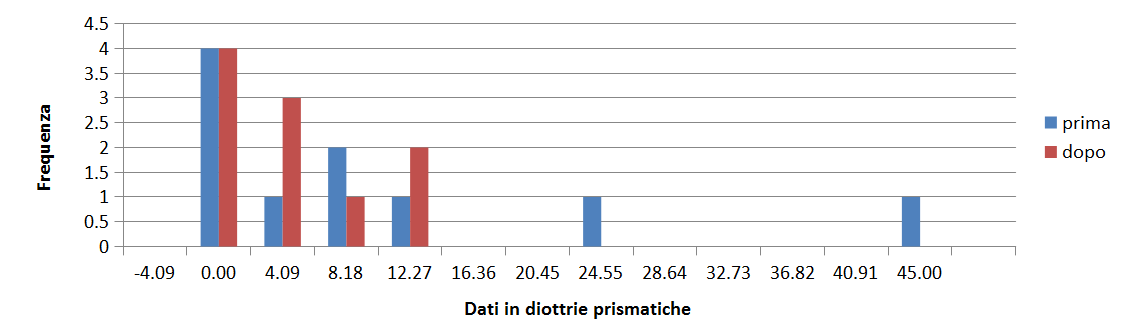
\includegraphics[scale=0.38]{source/grafici/COVER_TEST_7_TRATTATI_NUOVO.png}
	\caption[Istogramma gruppo sperimentale per cover test 7]{Istogramma gruppo sperimentale per cover test 7: confronto tra prima e seconda valutazione.}
	\label{fig:issuexample}
\end{figure}
\\\ \\\
 \begin{figure}[h!]
	\centering
	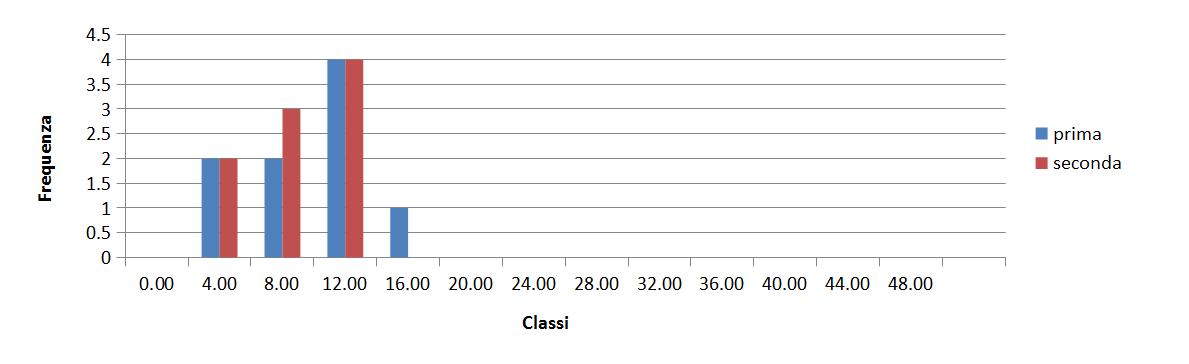
\includegraphics[scale=0.38]{source/grafici/cover_test_7_giustissimo_non_trattati.png}
	\caption[Istogramma gruppo di controllo per cover test 7]{Istogramma gruppo di controllo per cover test 7: confronto tra prima e seconda valutazione.}
	\label{fig:issuexample}
\end{figure}
\\\ \\\
\subsubsection{Cover test in posizione 8}

La posizione 8 corrisponde allo sguardo rivolto in alto a destra, stimolando i muscoli obliquo inferiore dell’occhio sinistro e il retto superiore dell’occhio destro. In questa posizione nel gruppo sperimentale 4 (40\%) soggetti ha riportato un miglioramento, 2 (20\%) sono rimasti invariati e 4 (40\%) sono peggiorati. Nel gruppo di controllo nessun (0\%) soggetto è migliorato, uno (11,1\%) è rimasto invariato e 8 (88,8\%) soggetti sono peggiorati. Come per il cover test 7 sono state riportati i valori medi nella Tabella 3.14 e 3.15 e gli istogrammi di Figura 3.20 e 3.21 rappresentano i dati ricavati durante la prima e seconda visita.

Il test di Wilcoxon un W-value di 15 con un valore critico di 4. Il cambiamento risulta quindi non significativo. Confrontando i dati del gruppo sperimentale e il gruppo di controllo si nota come, a differenza dei precedenti test, non è possibile riscontrare il miglioramento nella maggior parte dei soggetti trattati, ma è interessante notare come il gruppo non sottoposto a trattamento sia per l’88,8\% peggiorato. Anche gli istogrammi mostrano ancora lo spostamento dei dati della seconda visita verso valori inferiori. 

Il motivo per cui i cambiamenti nei cover test non sono risultati statisticamente significativi può essere attribuito, come per PPC, oltre alla ridotta ampiezza del campione, anche alla variabile della stanchezza.

%%%%%%%%%%%%%%%%%%
\begin{table}
\centering
\setlength\tabcolsep{4pt}
\begin{minipage}{0.48\textwidth}
\centering
\tablewidth=\textwidth

\begin{tabular}{|c|c|c|} \hline
{\textbf{}} & {\textbf{  \hspace{8pt}Prima\hspace{8pt} }} & {\textbf{ \hspace{8pt}Dopo\hspace{8pt}  }}\\ \hline
\textbf{Numeri dati} & 10 & 10 \\ 
\textbf{Media} & 14.10 & 9.60 \\  
\textbf{Dev. Std.} & 14.84 & 6.02 \\  
\textbf{Mediana} & 12.00 & 8.00 \\ 
\textbf{Moda} & 0.00 & 8.00 \\ 
\textbf{Errore Std.} & 15.74 & 6.28 \\ 
\hline
\end{tabular}
\caption{Dati gruppo sperimentale Cover test 8.}

\label{tab:accuracy} 
\end{minipage}%
\hfill
\begin{minipage}{0.48\textwidth}
\centering

\begin{tabular}{|c|c|c|} \hline
{\textbf{}} & {\textbf{  \hspace{8pt}Prima\hspace{8pt} }} & {\textbf{ \hspace{8pt}Dopo\hspace{8pt}  }}\\ \hline
\textbf{Numeri dati} & 9 & 9 \\ 
\textbf{Media} & 10.00 & 15.89 \\  
\textbf{Dev. Std.} & 6.08 & 8.34 \\  
\textbf{Mediana} & 8.00 & 16.00 \\  
\textbf{Moda} & 8.00 & \textbackslash \\
\textbf{Errore Std.} & 6.17 & 8.92 \\
\hline
\end{tabular}
\caption{Dati gruppo di controllo Cover test 8.}

 \label{tab:ompdiff} 
\end{minipage}
\end{table}
%%%%%%%%%%%%%%%%%%%%%
 \begin{figure}[h!]
	\centering
	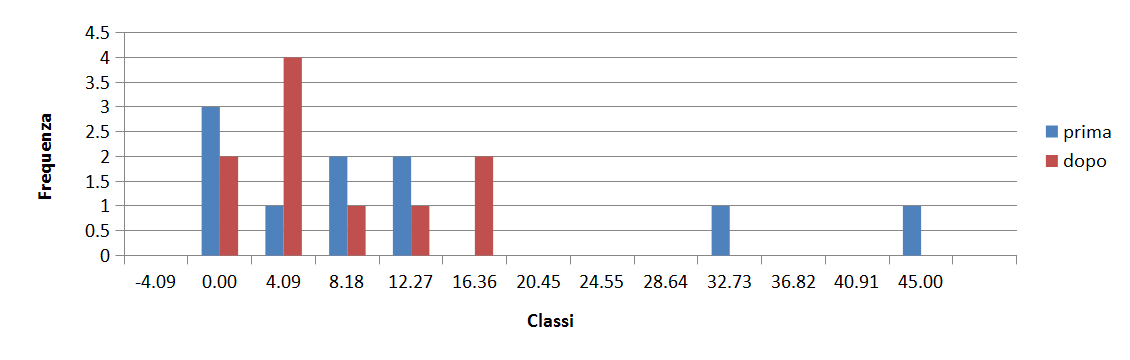
\includegraphics[scale=0.38]{source/grafici/cover_test_8_trattati_nuovo.png}
	\caption[Istogramma gruppo sperimentale per Cover test 8]{Istogramma gruppo sperimentale per Cover test 8: confronto tra prima e seconda valutazione.}
	\label{fig:issuexample}
\end{figure}
 \begin{figure}[h!]
	\centering
	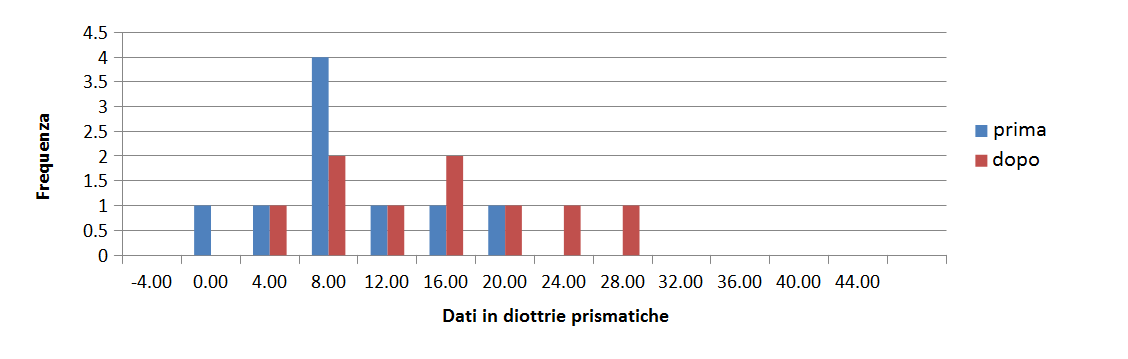
\includegraphics[scale=0.38]{source/grafici/cover_test_8_giustissimo_non_trattati.png}
	\caption[Istogramma gruppo di controllo per Cover test 8]{Istogramma gruppo di controllo per Cover test 8: confronto tra prima e seconda valutazione.}
	\label{fig:issuexample}
\end{figure}
\\\ \\\
\subsubsection{Stereopsi vicino}

I valori della stereopsi vicino sono riportati in appendice. Nel gruppo sperimentale è stato possibile riscontrare un miglioramento in 6 soggetti (60\%), 4 soggetti (40\%) sono rimasti invariati e nessuno (0\%) è peggiorato. Nel gruppo di controllo sono migliorati 4 soggetti (44,4\%), rimasti invariati 4 soggetti (44,4\%) e uno (11,1\%) è peggiorato. Nella Tabella 3.16 e 3.17 sono riportati i valori medi. In Figura 3.22 e 3.23 sono riportati gli istogrammi con il confronto tra prima e seconda valutazione in soggetti trattati e non trattati.

Il test di Wilcoxon fornisce un W-value di 0 con valore critico a 0. Il cambiamento è quindi da considerarsi significativo. Infatti in questo test è evidente la presenza di un cambiamento anche negli istogrammi riportati e nei valori medi. Inoltre è possibile osservare come nel gruppo sottoposto al trattamento il 60\% dei soggetti abbia riscontrato un miglioramento che ha portato 9 soggetti su 10 a vedere tutti i cerchi in rilievo e nessuno sia peggiorato. 
%%%%%%%%%%%%%%%%%%
\begin{table}
\centering
\setlength\tabcolsep{4pt}
\begin{minipage}{0.48\textwidth}
\centering
\tablewidth=\textwidth

\begin{tabular}{|c|c|c|} \hline
{\textbf{}} & {\textbf{  \hspace{8pt}Prima\hspace{8pt} }} & {\textbf{ \hspace{8pt}Dopo\hspace{8pt}  }}\\ \hline
\textbf{Numeri dati} & 10 & 10 \\ 
\textbf{Media} & 138.00 & 44.00 \\  
\textbf{Dev. Std.} & 146.20 & 12.65 \\  
\textbf{Mediana} & 70.00 & 40.00 \\ 
\textbf{Moda} & 40.00 & 40.00 \\ 
\textbf{Errore Std.} & 154.53 & 11.44 \\ 
\hline
\end{tabular}
\caption{Dati gruppo sperimentale Stereopsi vicino.}

\label{tab:accuracy} 
\end{minipage}%
\hfill
\begin{minipage}{0.48\textwidth}
\centering

\begin{tabular}{|c|c|c|} \hline
{\textbf{}} & {\textbf{  \hspace{8pt}Prima\hspace{8pt} }} & {\textbf{ \hspace{8pt}Dopo\hspace{8pt}  }}\\ \hline
\textbf{Numeri dati} & 9 & 9 \\ 
\textbf{Media} & 180.00 & 148.89 \\  
\textbf{Dev. Std.} & 172.55 & 153.33 \\  
\textbf{Mediana} & 50.00 & 40.00 \\  
\textbf{Moda} & 40.00 & 40.00 \\
\textbf{Errore Std.} & 154.99 & 147.63 \\
\hline
\end{tabular}
\caption{Dati gruppo di controllo Stereopsi vicino.}

 \label{tab:ompdiff} 
\end{minipage}
\end{table}
%%%%%%%%%%%%%%%%%%%%%
 \begin{figure}[h!]
	\centering
	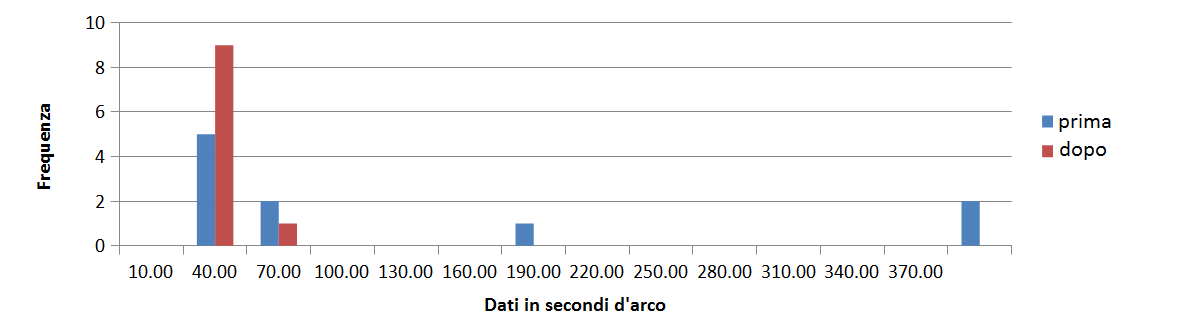
\includegraphics[scale=0.38]{source/grafici/STEREOPSI_VICINO_TRATTATI.png}
	\caption[Istogramma gruppo sperimentale per la Stereopsi vicino]{Istogramma gruppo sperimentale per la Stereopsi vicino: confronto tra prima e seconda valutazione.}
	\label{fig:issuexample}
\end{figure}
 \begin{figure}[h!]
	\centering
	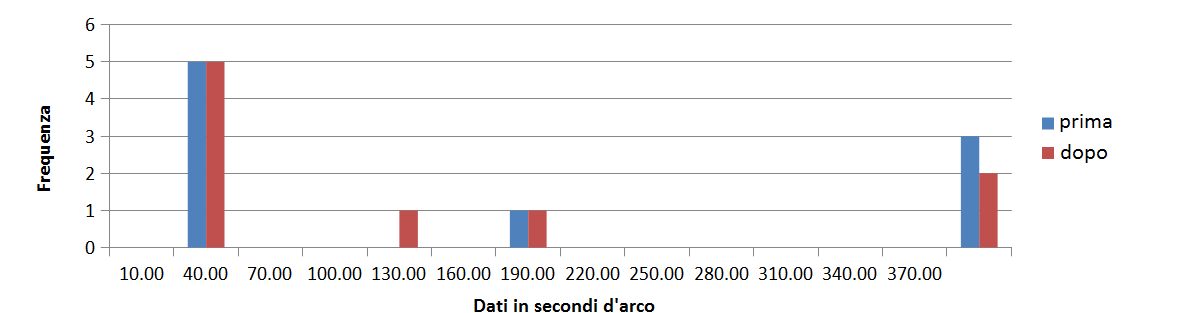
\includegraphics[scale=0.38]{source/grafici/STEREOPSI_VICINO_NON_TRATTATI.png}
	\caption[Istogramma gruppo di controllo per la Stereopsi vicino]{Istogramma gruppo di controllo per la Stereopsi vicino: confronto tra prima e seconda valutazione.}
	\label{fig:issuexample}
\end{figure}

\subsection{Analisi dei casi clinici}

Per concludere viene riportata la descrizione di due casi clinici maggiormente significativi dal punto di vista dei risultati ottenuti. Entrambi hanno effettuato il trattamento ma è stato applicato un differente impegno.
\\\ \\\
\textbf{Soggetto n°1: C.G. 14 anni, femmina}
\\\
Dopo la valutazione osteopatica-posturale, avvenuta il 6 settembre 2016, è stato possibile verificare che C.G. fosse affetta da deglutizione atipica con interposizione linguale e malocclusione in II classe dentale. È stata quindi inserita, per sua scelta, nel gruppo dei trattati e si è perciò sottoposta al trattamento logopedico-osteopatico per 3 mesi. Dall’analisi visiva effettuata il 15 settembre, prima del trattamento, e il 22 dicembre, dopo il trattamento, si sono ottenuti i dati della Tabella 3.18.

\begin{table}[H]
\begin{center}
\begin{tabular}{|c|c|c|} \hline
{\textbf{}} & {\textbf{Prima}} & {\textbf{Dopo}}\\ \hline
\textbf{Difetto refrattivo (D)} & +0,50 D (entrambi gli occhi) & 0 D entrambi gli occhi \\ \hline
\textbf{Foria L ($\Delta$)} & 1 eso & 0.50 eso \\ \hline
\textbf{Stereo L (sec d'arco)} & 30" & 30" \\ \hline
\textbf{PPC diritto (cm)} & 16 cm & 3 cm \\ \hline
\textbf{PPC alto (cm)} & 20 cm & 5 cm \\ \hline
\textbf{PPC basso (cm)} & 15 cm & 3 cm\\ \hline
\textbf{Foria V alto ($\Delta$)} & 0.50 exo & 0.50 exo \\ \hline
\textbf{Foria V diritto ($\Delta$)} & 1 exo & 1 exo \\ \hline
\textbf{Foria V basso ($\Delta$)} & 1 exo & 1 exo \\ \hline
\textbf{CT 1 ($\Delta$)} & 12 exo & 4 exo \\ \hline
\textbf{CT 2 ($\Delta$)} & 14 exo & 8 exo \\ \hline
\textbf{CT 3 ($\Delta$)} & 14 exo & 6 exo \\ \hline
\textbf{CT 4 ($\Delta$)} & 0 & 4 exo \\ \hline
\textbf{CT 5 ($\Delta$)} & 10 exo & 6 exo \\ \hline
\textbf{CT 6 ($\Delta$)} & 10 exo & 4 exo \\ \hline
\textbf{CT 7 ($\Delta$)} & 0 & 4 exo \\ \hline
\textbf{CT 8 ($\Delta$)} & 13 exo & 8 exo \\ \hline
\textbf{CT 9 ($\Delta$)} & 0 & 4 exo \\ \hline
\textbf{AA OD (D-cm)} & 14 D (7 cm) & 16.60 D (6 cm)\\ \hline
\textbf{AA OS (D-cm)} & 11 D (9 cm) & 14 D (7 cm)\\ \hline
\textbf{AA OO (D-cm)} & 16.60 D (6 cm) & 16.60 D (6 cm) \\ \hline
\textbf{Stereo V (sec d'arco)} & 80" & 40" \\ \hline
\textbf{DF (min d'arco)} & 6.90 exo & 6.90 exo\\ \hline
\textbf{MEM OD (D)} & 1.00 LAG  & 1.25 LAG \\ \hline
\textbf{MEM OS (D)} & 1.25 LAG & 1.25 LAG\\ \hline

\hline
\end{tabular}
\end{center}
\caption{Dati valutazione di C.G.}
\end{table}

I dati rivelano la presenza nella prima valutazione di disfunzioni del sistema visivo, soprattutto riguardo il punto prossimo di convergenza, il cover test nelle 9 posizioni di sguardo, la stereopsi vicino e la disparità di fissazione. Si potrebbe ipotizzare un'alterata funzione dei muscoli estrinseci dell’occhio per lo scompenso causato dalla deglutizione atipica e dalla malocclusione. Allo stesso modo è possibile ipotizzare che i valori fuori norma del cover test possano essere dovuti all’instabilità della visione binoculare, testimoniata anche dai valori della stereopsi e della disparità di fissazione. Presenta inoltre una leggera ipermetropia a entrambi gli occhi corretta con lenti oftalmiche. 

C.G. ha effettuato con costanza gli esercizi proposti dalla logopedista e si è presentata ogni settimana all’ambulatorio per il trattamento osteopatico. È stata rivalutata il 22 dicembre, dopo 3 mesi e la situazione è notevolmente migliorata. Il punto prossimo di convergenza si è avvicinato notevolmente e anche i valori del cover test si sono abbassati. Nella seconda valutazione quindi quasi tutti i valori sono rientrati nella norma e il soggetto può dirsi perciò complessivamente migliorato.
Si suppone che sia migliorata la stabilità del sistema visivo del soggetto, dal momento che migliora la capacità di mantenere singola la mira durante il PPC e questo può aver portato ad una maggiore consapevolezza dello spazio e quindi all’aumento del valore della stereopsi e alla riduzione dei valori del cover test. 

\chapter{Conclusioni e Sviluppi Futuri}

A conclusione della ricerca e dell’analisi statistica dei dati si osserva che, secondo il test di Wilcoxon, non esiste la correlazione tra molte funzioni del sistema visivo e l’apparato stomatognatico e che il cambiamento osservato sia da ritenersi casuale e non dovuto al trattamento logopedico-osteopatico.
 
Analizzando i valori medi è stato possibile riscontrare un riduzione dei valori nei test di Punto Prossimo di Convergenza (diritto e in basso), Cover test (a destra e in alto a destra) e Stereopsi vicino. Tra questi è stato osservato un cambiamento da considerarsi statisticamente significativo solo nel test della Stereopsi vicino. Il sistema visivo ha infatti trovato una migliore stabilità in seguito al trattamento all’apparato stomatognatico, permettendo una maggiore consapevolezza dello spazio e quindi un miglioramento della percezione della profondità. L’aumento della stereopsi può essere legato al perfezionamento della binocularità del soggetto e quindi alle altre funzioni in cui è presente il cambiamento come la convergenza e la stabilità dei muscoli oculari che influenzano le forie.
\\\

Per le funzioni analizzate è possibile che il cambiamento sia casuale, ma, dal confronto dei grafici del gruppo sperimentale e del gruppo di controllo, dal risultato ottenuto per la stereopsi e dal cambiamento dei singoli soggetti, è possibile ancora ipotizzare l’efficacia del trattamento logopedico-osteopatico effettuato su soggetti con primarietà linguale. Ciò che può essere affermato ora è che la rieducazione delle funzioni dell’apparato stomatognatico ha permesso al sistema visivo di trovare una nuova stabilità aumentando la percezione dello spazio.
\\\ \\\ \\\ \\\
In questa ricerca si è voluto effettuare l’analisi statistica considerando i soggetti come un gruppo, piuttosto che come singoli, poiché l’ampiezza del campione è stata ritenuta abbastanza grande per effettuare l’analisi statistica di Wilcoxon, \emph{ma}, sebbene l’approccio di  Wilcoxon  abbia confutato la tesi, i risultati mostrano comunque a un miglioramento che potrebbe essere reso visibile utilizzando un altro approccio. Perciò questo lavoro si pone come un un punto di partenza per nuovi tipi di analisi in modo da poter confermare o smentire i risulatati ottenuti con Wilcoxon.
\\\ \\\ \\\ \\\
\section{Sviluppi futuri}

Alla luce delle conclusioni sopradescritte si possono pensare a diversi sviluppi che continuino il lavoro già svolto. A questo scopo sono state pensate diverse alternative:
\begin{enumerate}
\item effettuare una statistica a caso singolo sui soggetti che hanno evidenziato il miglioramento, per poter smentire o confermare che il trattamento effettuato non è risultato efficace sul sistema visivo.
\item approfondire il cambiamento del punto prossimo di convergenza utilizzando un campione più ampio per comprendere quanto la disfunzione della deglutizione possa influire sulla convergenza. Si potrebbe, infatti, effettuare un confronto con quanto riportato in letteratura, dove si registra un cambiamento della convergenza agendo sulle mal occlusioni dentali.
\item valutare quanto il solo risultato del cover test possa essere influenzato dalla disfunzione stomatognatica e comprendere quanto questo test possa essere affidabile nel valutare la funzione della muscolatura estrinseca.
\item rieffettuare l’analisi di Wilcoxon con un campione più ampio, possibilmente concentrandosi sui test in cui questo studio ha riportato un miglioramento.
\end{enumerate}
\\\ \\\ \\\
Inoltre, affinché l’analisi sia affidabile il più possibile:
\begin{itemize}
\item si potrebbe ridurre la quantità di test da sottoporre, oppure utilizzare un diverso metodo. Ad esempio il cover test nelle 9 posizioni di sguardo si è rivelato molto stancante per i soggetti, perciò si potrebbe utilizzare un test più immediato come la Bernell Muscle Imbalance Measure sempre proposto nelle 9 posizioni di sguardo.
\item sarebbe preferibile sottoporre i soggetti ad un questionario riguardo la loro condizione di stanchezza prima di ogni valutazione optometrica, per assicurarsi che le valutazioni siano effettuate sotto le stesse condizioni.
\item supervisionare maggiormente il soggetto nell’esecuzione degli esercizi. Nella ricerca effettuata c’era una forte dipendenza dall’impegno quotidiano dei soggetti, i quali sono stati seguiti dalla laureanda e dalla logopedista attraverso la compilazione di un diario a casa e attraverso appuntamenti in ambulatorio.
\item usare un’alternativa al Cover test per indagare le funzioni muscolari. Essendo un test che valuta qualitativamente la binocularità del soggetto, non è possibile determinare se il risultato ottenuto sia dovuto a disfunzioni muscolari o a uno squilibrio della visione binoculare. Esso è stato utilizzato perché si è ritenuto che per aver una binucularità perfetta sarebbe necessario possedere una corretta percezione dello spazio integrata con un buona stabilità muscolare e il cover test può fornire dati precisi e fini, quindi confrontabili, dal momento che indaga la presenza di forie\footnote{Piero Silvestrini Biavati: \emph{La postura del capo nella patogenesi dello squilibrio posturale, ruolo dell occlusione dentale e del sistema visivo}}. Però l’alterata percezione spaziale non è una variabile controllabile durante lo svolgimento del cover test, per questo si potrebbe tentare di utilizzare un test come il DEM o NSUCO, che permettono una valutazione quantitativa, anche se non precisa, delle abilità dei muscoli oculari e valutare se queste rimangono le stesse o migliorano.
\end{itemize}


\begin{appendices}
\chapter{Risultati dei test}
%\section{PPC diritto}

\begin{table}[H]
\begin{center}
\begin{tabular}{|c|c|c|c|c|c|c|} \hline
{\textbf{}} & \pbox{20cm}{\textbf{Rottura} \\ \textbf{prima}} & \pbox{20cm}{\textbf{Rottura} \\ \textbf{dopo}} & \textbf{Differenza} & \pbox{20cm}{\textbf{Recupero} \\ \textbf{prima}} & \pbox{20cm}{\textbf{Recupero} \\ \textbf{dopo}} & \textbf{Differenza} \\ \hline
\textbf{S. 1} & 8 & 9 & -1 & 14 & 13 & 1 \\ \hline
\textbf{S. 2} & 13 & 0 & 3 & 5 & 0 & 5 \\ \hline
\textbf{S. 3} & 16 & 3 & 13 & 28 & 3 & 25  \\ \hline
\textbf{S. 4} & 13 & 0 & 13 & 23 & 0 & 23  \\ \hline
\textbf{S. 5} & 2 & 6 & -4 & 4 & 25 & -21  \\ \hline
\textbf{S. 6} & 7 & 5 & 2 & 10 & 8 & 2 \\ \hline
\textbf{S. 7} & 40 & 7 & 33 & 40 & 9 & 31 \\ \hline
\textbf{S. 8} & 4 & 8 & -4 & 8 & 10 & -2  \\ \hline
\textbf{S. 9} & 3 & 5 & -2 & 8 & 6 & 2 \\ \hline
\textbf{S. 10} & 0 & 0 & 0 & 2 & 0 & 2 \\ \hline

\end{tabular}
\end{center}
\caption{Dati PPC diritto del gruppo sperimentale}
\end{table}
\\\ \\\ \\\ \\\ \\\ \\\ \\\ \\\ \\\ \\\ \\\ \\\ \\\ \\\

\begin{table}[H]
\begin{center}
\begin{tabular}{|c|c|c|c|c|c|c|} \hline
{\textbf{}} & \pbox{20cm}{\textbf{Rottura} \\ \textbf{prima}} & \pbox{20cm}{\textbf{Rottura} \\ \textbf{dopo}} & \textbf{Differenza} & \pbox{20cm}{\textbf{Recupero} \\ \textbf{prima}} & \pbox{20cm}{\textbf{Recupero} \\ \textbf{dopo}} & \textbf{Differenza} \\ \hline
\textbf{S. 1} & 0 & 0 & 0 & 0 & 0 & 0 \\ \hline
\textbf{S. 2} & 10 & 16 & -6 & 18 & 20 & 2 \\ \hline
\textbf{S. 3} & 0 & 1 & -1 & 0 & 2 & -2 \\ \hline
\textbf{S. 4} & 5 & 7 & -2 & 9 & 10 & -1 \\ \hline
\textbf{S. 5} & 0 & 4 & -4 & 0 & 8 & -8 \\ \hline
\textbf{S. 6} & 45 & 5 & 40 & 50 & 8 & 42  \\ \hline
\textbf{S. 7} & 6 & 3 & 3 & 9 & 6 & 3 \\ \hline
\textbf{S. 8} & 17 & 17 & 0 & 27 & 22 & 5 \\ \hline
\textbf{S. 9} & 6 & 14 & -8 & 9 & 17 & -8 \\ \hline
\end{tabular}
\end{center}
\caption{Dati PPC diritto del gruppo di controllo}
\end{table}

\\\ \\\  

%\section{PPC basso}

\begin{table}[H]
\begin{center}
\begin{tabular}{|c|c|c|c|c|c|c|} \hline
{\textbf{}} & \pbox{20cm}{\textbf{Rottura} \\ \textbf{prima}} & \pbox{20cm}{\textbf{Rottura} \\ \textbf{dopo}} & \textbf{Differenza} & \pbox{20cm}{\textbf{Recupero} \\ \textbf{prima}} & \pbox{20cm}{\textbf{Recupero} \\ \textbf{dopo}} & \textbf{Differenza} \\ \hline
\textbf{S. 1} & 1 & 4 & -3 & 4 & 8 & -4 \\ \hline
\textbf{S. 2} & 5 & 0 & 5 & 7 & 0 & 7 \\ \hline
\textbf{S. 3} & 15 & 3 & 12 & 29 & 7 & 22  \\ \hline
\textbf{S. 4} & 17 & 0 & 17 & 27 & 0 & 27  \\ \hline
\textbf{S. 5} & 0 & 4 & -4 & 0 & 12 & -12  \\ \hline
\textbf{S. 6} & 0 & 0 & 0 & 0 & 0 & 0 \\ \hline
\textbf{S. 7} & 40 & 0 & 40 & 40 & 0 & 40 \\ \hline
\textbf{S. 8} & 0 & 0 & 0 & 0 & 0 & 0 \\ \hline
\textbf{S. 9} & 0 & 0 & 0 & 0 & 0 & 0 \\ \hline
\textbf{S. 10} & 0 & 0 & 0 & 0 & 0 & 0 \\ \hline

\end{tabular}
\end{center}
\caption{Dati PPC basso del gruppo sperimentale}
\end{table}
\\\ \\\ \\\ \\\ \\\ \\\ \\\ \\\ \\\ \\\ \\\ 

\begin{table}[H]
\begin{center}
\begin{tabular}{|c|c|c|c|c|c|c|} \hline
{\textbf{}} & \pbox{20cm}{\textbf{Rottura} \\ \textbf{prima}} & \pbox{20cm}{\textbf{Rottura} \\ \textbf{dopo}} & \textbf{Differenza} & \pbox{20cm}{\textbf{Recupero} \\ \textbf{prima}} & \pbox{20cm}{\textbf{Recupero} \\ \textbf{dopo}} & \textbf{Differenza} \\ \hline
\textbf{S. 1} & 0 & 0 & 0 & 0 & 0 & 0 \\ \hline
\textbf{S. 2} & 13 & 15 & -2 & 18 & 18 & 0 \\ \hline
\textbf{S. 3} & 0 & 0 & 0 & 0 & 0 & 0 \\ \hline
\textbf{S. 4} & 4 & 3 & 1 & 10 & 6 & 4 \\ \hline
\textbf{S. 5} & 0 & 6 & -6 & 0 & 17 & -17 \\ \hline
\textbf{S. 6} & 45 & 6 & 39 & 50 & 10 & 40  \\ \hline
\textbf{S. 7} & 4 & 6 & -2 & 10 & 9 & 1 \\ \hline
\textbf{S. 8} & 5 & 4 & 1 & 8 & 7 & 1 \\ \hline
\textbf{S. 9} & 0 & 19 & -19 & 0 & 23 & -23 \\ \hline
\end{tabular}
\end{center}
\caption{Dati PPC basso del gruppo di controllo}
\end{table}

\\\ \\\  

%\section{Cover test 7}
%%%%%%%%%%%%%%%%%%
\begin{table}[H]
\centering
\setlength\tabcolsep{4pt}
\begin{minipage}{0.48\textwidth}
\centering
\tablewidth=\textwidth

\begin{tabular}{|c|c|c|c|} \hline
{\textbf{}} & {\textbf{Prima}} & {\textbf{Dopo}}& {\textbf{Differenza}} \\ \hline
\textbf{S. 1} & 9 x & 6 x & 3 \\ \hline
\textbf{S. 2} & 25 x & 14 x & 11 \\ \hline
\textbf{S. 3} & 0 & 4 x & -4 \\ \hline
\textbf{S. 4} & 0 & 4 x & -4 \\ \hline
\textbf{S. 5} & 2 x & 14 x & -12 \\ \hline
\textbf{S. 6} & 45 x & 2 x & 43 \\ \hline
\textbf{S. 7} & 14 x & 12 x & 2 \\ \hline
\textbf{S. 8} & 2 x & 2 x & 0 \\ \hline
\textbf{S. 9} & 8 x & 6 x & 2 \\ \hline
\textbf{S. 10} & 12 x & 6 x & 6 \\ \hline
\end{tabular} 
\caption{Dati Cover test 7 del gruppo sperimentale}

\label{tab:accuracy} 
\end{minipage}%
\hfill
\begin{minipage}{0.48\textwidth}
\centering

\begin{tabular}{|c|c|c|c|} \hline
{\textbf{}} & {\textbf{Prima}} & {\textbf{Dopo}}& {\textbf{Differenza}} \\ \hline
\textbf{S. 1} & 4 x & 8 x & -4 \\ \hline
\textbf{S. 2} & 12 x & 12 x & 0 \\ \hline
\textbf{S. 3} & 8 x & 6 x & 2 \\ \hline
\textbf{S. 4} & 14 x & 14 x & 0 \\ \hline
\textbf{S. 5} & 12 s & 14 s & -2 \\ \hline
\textbf{S. 6} & 6 s  & 8 s  & -2 \\ \hline
\textbf{S. 7} & 9 x & 8 x & 1 \\ \hline
\textbf{S. 8} & 14 x & 14 x & 0 \\ \hline
\textbf{S. 9} & 18 x & 6 x & 12 \\ \hline
\end{tabular} 
\caption{Dati Cover test 7 del gruppo di controllo}

 \label{tab:ompdiff} 
\end{minipage}
\end{table}
%%%%%%%%%%%%%%%%%%%%%
\\\ \\\ \\\ \\\ \\\ \\\ \\\ 
%\section{Cover test 8}
%%%%%%%%%%%%%%%%%%
\begin{table}[H]
\centering
\setlength\tabcolsep{4pt}
\begin{minipage}{0.48\textwidth}
\centering
\tablewidth=\textwidth

\begin{tabular}{|c|c|c|c|} \hline
{\textbf{}} & {\textbf{Prima}} & {\textbf{Dopo}}& {\textbf{Differenza}} \\ \hline
\textbf{S. 1} & 0 & 6 x & -6 \\ \hline
\textbf{S. 2} & 35 x & 18 x & 17 \\ \hline
\textbf{S. 3} & 13 x & 8 x & 5 \\ \hline
\textbf{S. 4} & 0 & 0 & 0 \\ \hline
\textbf{S. 5} & 2 x & 10 x & -8 \\ \hline
\textbf{S. 6} & 45 x & 4 x & 41 \\ \hline
\textbf{S. 7} & 12 x & 16 x & -4 \\ \hline
\textbf{S. 8} & 8 x & 8 x & 0 \\ \hline
\textbf{S. 9} & 12 x & 18 x & -6 \\ \hline
\textbf{S. 10} & 14 x & 8 x & 6 \\ \hline
\end{tabular} 
\caption{Dati Cover test 8 del gruppo sperimentale}

\label{tab:accuracy} 
\end{minipage}%
\hfill
\begin{minipage}{0.48\textwidth}
\centering

\begin{tabular}{|c|c|c|c|} \hline
{\textbf{}} & {\textbf{Prima}} & {\textbf{Dopo}}& {\textbf{Differenza}} \\ \hline
\textbf{S. 1} & 10 x & 16 x & -6 \\ \hline
\textbf{S. 2} & 20 x & 20 x & 0 \\ \hline
\textbf{S. 3} & 6 x & 8 x & -2 \\ \hline
\textbf{S. 4} & 18 x & 30 x & -12 \\ \hline
\textbf{S. 5} & 8 s & 12 s & -4 \\ \hline
\textbf{S. 6} & 0  & 4 s & -4 \\ \hline
\textbf{S. 7} & 8 x & 10 x & -2 \\ \hline
\textbf{S. 8} & 8 x & 25 x & -17 \\ \hline
\textbf{S. 9} & 12 x & 18 x & -6 \\ \hline
\end{tabular} 
\caption{Dati Cover test 8 del gruppo di controllo}

 \label{tab:ompdiff} 
\end{minipage}
\end{table}
%%%%%%%%%%%%%%%%%%%%%

%\section{Stereopsi vicino}
\\\ \\\ \\\
%%%%%%%%%%%%%%%%%%
\begin{table}[H]
\centering
\setlength\tabcolsep{4pt}
\begin{minipage}{0.48\textwidth}
\centering
\tablewidth=\textwidth

\begin{tabular}{|c|c|c|c|} \hline
{\textbf{}} & {\textbf{Prima}} & {\textbf{Dopo}}& {\textbf{Differenza}} \\ \hline
\textbf{S. 1} & 400" & 40" & 360 \\ \hline
\textbf{S. 2} & 40" & 40" & 0 \\ \hline
\textbf{S. 3} & 80" & 40" & 40 \\ \hline
\textbf{S. 4} & 200" & 40" & 160 \\ \hline
\textbf{S. 5} & 80" & 40" & 40 \\ \hline
\textbf{S. 6} & 40" & 40" & 0 \\ \hline
\textbf{S. 7} & 60" & 40" & 20 \\ \hline
\textbf{S. 8} & 40" & 40" & 0 \\ \hline
\textbf{S. 9} & 40" & 40" & 0 \\ \hline
\textbf{S. 10} & 400" & 80" & 320 \\ \hline
\end{tabular} 
\caption{Dati Stereopsi vicino del gruppo sperimentale}

\label{tab:accuracy} 
\end{minipage}%
\hfill
\begin{minipage}{0.48\textwidth}
\centering

\begin{tabular}{|c|c|c|c|} \hline
{\textbf{}} & {\textbf{Prima}} & {\textbf{Dopo}}& {\textbf{Differenza}} \\ \hline
\textbf{S. 1} & 50" & 40" & 10 \\ \hline
\textbf{S. 2} & 50" & 40" & 10 \\ \hline
\textbf{S. 3} & 40" & 40" & 0 \\ \hline
\textbf{S. 4} & 40" & 40" & 0 \\ \hline
\textbf{S. 5} & 400" & 400" & 0 \\ \hline
\textbf{S. 6} & 400" & 140" & 260 \\ \hline
\textbf{S. 7} & 200" & 200" & -200\\ \hline
\textbf{S. 8} & 40" & 40" & 0 \\ \hline
\textbf{S. 9} & 400" & 200" & 200 \\ \hline
\end{tabular} 
\caption{Dati Stereopsi vicino del gruppo di controllo}

 \label{tab:ompdiff} 
\end{minipage}
\end{table}
%%%%%%%%%%%%%%%%%%%%%





\end{appendices}

\begin{appendices}
\chapter{Schede di valutazione}

Nome e cognome: \_\_\_\_\_\_\_\_\_\_\_\_\_\_\_\_\_\_\_\_\_\_\_\_\_\_ \  Età:\_\_\_\_\_\_
\\\ \\\
\textbf{1$^{\circ}$visita:}  \ \ / \    /
\\\
\textbf{2$^{\circ}$visita:}  \ \ / \    /
\\\ \\\ \\\
\underline{\textbf{TEST LONTANO}}
\\\ \\\
\textbf{Distanza Interpupillare:}
\\\
OD: \_\_\_\_\_\_\_\_\_\_\_\_\_
\\\
OS: \_\_\_\_\_\_\_\_\_\_\_\_\_
\\\
OO: \_\_\_\_\_\_\_\_\_\_\_\_\_
\\\ \\\
\textbf{Refrazione:}
\\\
metodo: \_\_\_\_\_\_\_\_\_\_\_
\\\
Massimo positivo:
\\\
OD: sf \_\_\_\_\_\_\_\_ cil \_\_\_\_\_\_\_\_ asse \_\_\_\_\_\_\_\_ AV: \_\_\_\_\_\_\_\_ /10
\\\
OS: sf \_\_\_\_\_\_\_\_ cil \_\_\_\_\_\_\_\_ asse \_\_\_\_\_\_\_\_ AV: \_\_\_\_\_\_\_\_ /10
\\\
Minimo positivo:
\\\
OD: sf \_\_\_\_\_\_\_\_ cil \_\_\_\_\_\_\_\_ asse \_\_\_\_\_\_\_\_ AV: \_\_\_\_\_\_\_\_ /10
\\\
OS: sf \_\_\_\_\_\_\_\_ cil \_\_\_\_\_\_\_\_ asse \_\_\_\_\_\_\_\_ AV: \_\_\_\_\_\_\_\_ /10
\\\
Velocità:
\begin{table}[H]
\begin{tabular}{|c|c|c|} \hline
{\textbf{1}} & {\textbf{2}} & {\textbf{3}}\\ \hline
\end{tabular}
\end{table}
\\\ \\\
\textbf{Stereopsi Lontano:} \_\_\_\_\_\_\_\_
\\\ \\\
\textbf{Foria:} \_\_\_\_\_\_\_\_\_\_\_\_\_\_\_\_\_
\\\ \\\ \\\ \\\ \\\
\underline{\textbf{TEST VICINO}}
\\\ \\\
\textbf{PPC:}
\begin{table}[H]
\begin{tabular}{|c|c|c|c|} \hline
{\textbf{}} & {\textbf{Rott/Rec}} & {\textbf{Rott/Rec}}& {\textbf{Rott/Rec}}\\ \hline
\textbf{Pos. Diritto} & &  &  \\ \hline
\textbf{Pos. Alto} &  &  &  \\ \hline
\textbf{Pos. Basso} &  &  &  \\ \hline
\end{tabular}
\end{table}
\\\ \\\
fatica:
\begin{table}[H]
\begin{tabular}{|c|c|c|c|c|} \hline
{\textbf{1}} & {\textbf{2}} & {\textbf{3}} & {\textbf{4}} & {\textbf{5}}\\ \hline
\end{tabular}
\end{table}
\\\ \\\
soppressione: \_\_\_\_\_\_\_\_
\\\
deviazione: \_\_\_\_\_\_\_\_\_
\\\ \\\
\textbf{Forie:} 
\\\ 
metodo: \_\_\_\_\_\_\_\_\_\_\_
\begin{table}[H]
\begin{tabular}{|c|} \hline
{\textbf{Pos. Diritto \ \ \ \ \ \ \ \ \ \ \ \ \ \ \ \ \ \ \ \ \ \ \ } \\ \hline
\textbf{Pos. Alto \ \ \ \ \ \ \ \ \ \ \ \ \ \ \ \ \ \ \ \ \  \ \ \ \ \ } \\ \hline
\textbf{Pos. Basso \ \ \ \ \ \ \ \ \ \ \ \ \ \ \ \ \ \ \ \ \ \ \ \ } \\ \hline
\end{tabular}
\end{table}
\\\ \\\
fatica:
\begin{table}[H]
\begin{tabular}{|c|c|c|c|c|} \hline
{\textbf{1}} & {\textbf{2}} & {\textbf{3}} & {\textbf{4}} & {\textbf{5}}\\ \hline
\end{tabular}
\end{table}
\\\ \\\ \\\
\textbf{Cover test:}
\begin{table}[H]
\begin{tabular}{|c|c|c|c|c|c|c|c|c|c|} \hline
{\textbf{}} & {\ \ \textbf{1}\ \ } & {\ \ \textbf{2}\ \ } & {\ \ \textbf{3}\ \ } & {\ \ \textbf{4}\ \ } & {\ \ \textbf{5}\ \ } & {\ \ \textbf{6}\ \ } & {\ \ \textbf{7}\ \ } & {\ \ \textbf{8}\ \ } & {\ \ \textbf{9}\ \ \ }\\ \hline
\textbf{EXO}} &  &  &  &  &  &  &  &  & \\ \hline
\textbf{ESO}}  &  &  &  &  &  &  &  &  & \\ \hline
\end{tabular}
\end{table}

 \begin{figure}[h!]
	\centering
	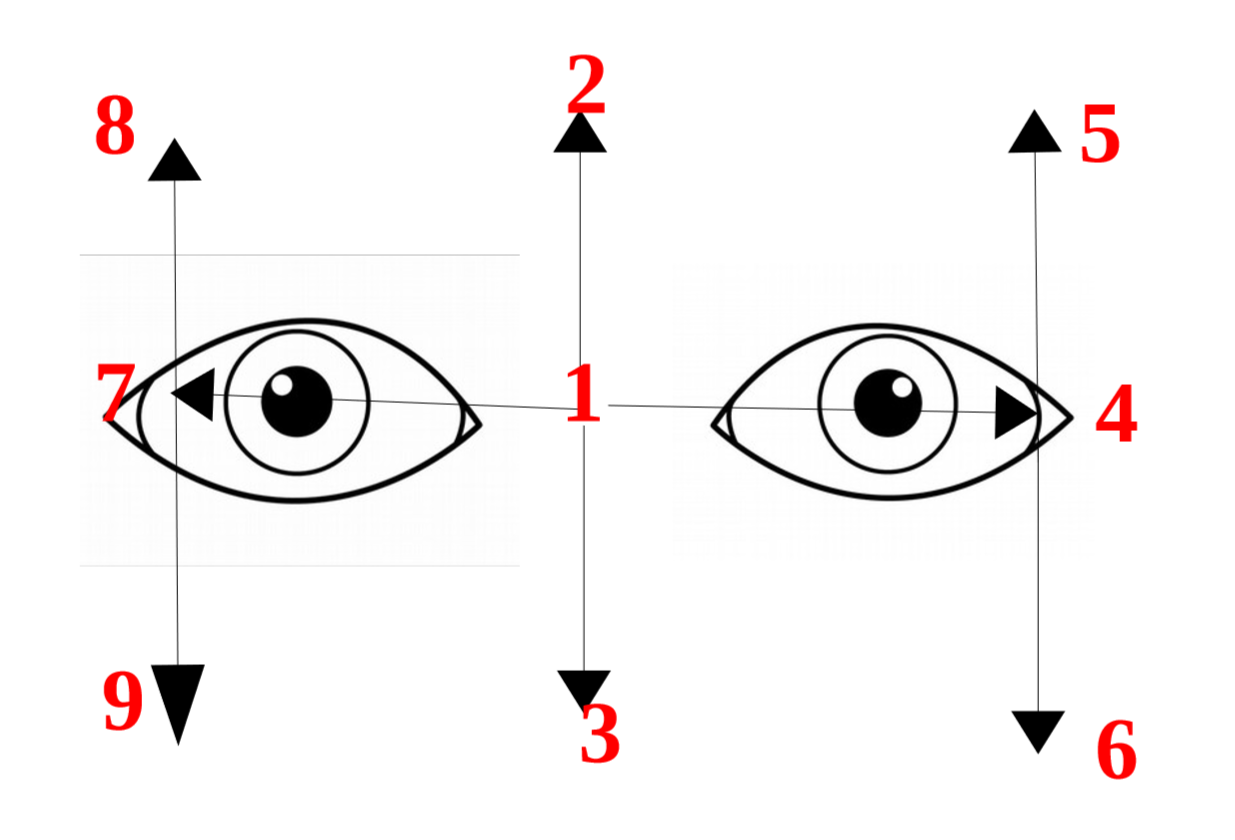
\includegraphics[scale=0.27]{source/immagini/posizioni_cover_test.png}
	\label{fig:issuexample}
\end{figure}
\\\ \\\
fatica:
\begin{table}[H]
\begin{tabular}{|c|c|c|c|c|} \hline
{\textbf{1}} & {\textbf{2}} & {\textbf{3}} & {\textbf{4}} & {\textbf{5}}\\ \hline
\end{tabular}
\end{table}
\\\ \\\
\textbf{AA}:
\\\
metodo: \_\_\_\_\_\_\_\_
\\\
\begin{table}[H]
\begin{tabular}{|c|c|c|c|} \hline
{\textbf{OD}} & {\ \ \ \ \ \ \ \ \ }  & {\ \ \ \ \ \ \ \ \ } & {\ \ \ \ \ \ \ \ \ } \\ \hline
\textbf{OS} & &  &  \\ \hline
\textbf{OO} &  &  &  \\ \hline
\end{tabular}
\end{table}
\\\ \\\
fatica:
\begin{table}[H]
\begin{tabular}{|c|c|c|c|c|} \hline
{\textbf{1}} & {\textbf{2}} & {\textbf{3}} & {\textbf{4}} & {\textbf{5}}\\ \hline
\end{tabular}
\end{table}
\\\ \\\
\textbf{Disparità di fissazione}: \_\_\_\_\_\_\_\_
\\\
\textbf{Stereopsi}: \_\_\_\_\_\_\_\_\_\_\_\_\_\_\_\_\_
\\\
\textbf{MEM}: 
\\\
OD: \_\_\_\_\_\_\_\_
\\\
OS: \_\_\_\_\_\_\_\_

\end{appendices}

\begin{thebibliography}{9}
\addcontentsline{toc}{chapter}{Bibliografia}

\bibitem{bib1}
Giorgetti, Deodato, Malpassi: \emph{Occlusione vs oculomotricità: stato dell’arte}

\bibitem{bib2}
Angelo Bairati: \emph{Trattato di anatomia umana – sistema nervoso periferico, organi di senso, apparato tegumentario}, II edizione, Volume III, Edizioni Minerva Medica

\bibitem{bib3}
G.C. Balboni, A. Bastianini, E. Brizzi, L. Comparini, G. Filogamo, G. Giordano-Lanza, C. E. Grossi, F. A. Manzoli, G. Marinozzi, P. Motta, G. E. Orlandini, A. Passaponti, E. Reale, A. Ruggeri, A. Santoro, D. Zaccheo \emph{Anatomia Umana 3}, edizioni edi.ermes

\bibitem{bib4}
William J.: \emph{Butterworth Heinemann Elsevier “Borish’s Clinical Refraction} Benjamin ed.

\bibitem{bib5}
A. Cuccia, C. Caradonna: \emph{The relationship between the stomatognathic system and body posture}, 2009

\bibitem{bib6}
Philippe Caiazzo: \emph{TOP terapia osteopatico-posturale}, edizioni Marrapese, editore-Roma

\bibitem{bib7}
R. Ciancaglini, R. Gelmetti, E. Lazzari: \emph{Evoluzione degli studi sulla relazione tra occlusione e postura}, da Mondo Ortodontico gennaio, 2008

\bibitem{bib8}
Rhoda P. Erhardt, \emph{Developmental Visual Dysfunction: Models for Assessment and Management}, capitolo 3, Erhardt Developmental Products 1990.

\bibitem{bib9}
Mautone Salvatore: \emph{“Sistema Tonico posturale: il direttore d’orchestra!”}

\bibitem{bib10}
David B. Elliott: \emph{Clinical procedures in primary eye care}, Elsevier Saunders Fourth Edition, 2014

\bibitem{bib11}
Bruno Garuffo: Materiale Didattico del corso Tecniche Fisiche per l’Optometria Generale II modulo, 2014-2015

\bibitem{bib12}
Marzia Lecchi: Materiale Didattico del corso Fisiologia Generale ed Oculare II modulo, 2013-2014.

\bibitem{bib13}
Mauro Faini: \emph{Lezioni di optometria}

\bibitem{bib14}
Corinna Galbero: \emph{Influenza della dominanza oculare sull’equilibrio posturale in soggetti giovani}, tesi di laurea in Ottica e Optometria dell’Università di Padova 

\bibitem{bib15}
Alice Delbono: \emph{Correlazione tra squilibrio muscolare oro-facciale e disfunzioni di interesse osteopatico: studio su 21 soggetti}, tesi di laurea in Logopedia, 2015

\bibitem{bib16}
Maria Cristina Fresa: \emph{Deglutizione fisiologica, deglutizione disfunzionale, significato neurofisiologico della deglutizione e sua interferenza sulla postura}, tesi di laurea in Medicina e Chirurgia dell’Università di Pisa, specializzazione in Medicina fisica e riabilitativa, 2011

\bibitem{bib17}
http://www.gruppocdc.it/pazienti/prestazioni/laboratorio-analisi-cliniche/chimica-clinica-tossicologica/7-cdc/cdc-ita/314-trattamento-dello-squilibrio-muscolare-oro-facciale

\bibitem{bib18}
https://alessandrogarlinzoni.wordpress.com/2016/10/28/perche-locchio-influenza-la-postura/

\bibitem{bib19}
Wikipedia, www.wikipedia.org

\end{thebibliography} 

\chapter*{Ringraziamenti}
\addcontentsline{toc}{chapter}{Ringraziamenti}

sasmri!


\end{document}